\section{Results}\label{sec:results}

\subsection{BP SB-FET Model Validation and Device Characterization}\label{sec:res_model}

The native behavioral library \texttt{bp\_ari\_ngspice.lib} (\texttt{v2}) accurately reproduced the experimental transfer and output surfaces across the entire measured operating plane. Table~\ref{tab:device_metrics} summarizes the electrical parameters extracted at $|V_{ds}| = 0.8\ \text{V}$, exhibiting mean relative errors against the experimental LUTs of only $0.0621\%$ in \textit{n-FET} mode and $0.0032\%$ in \textit{p-FET} mode. Note that the extracted subthreshold swing ($106.59\text{--}148.08\ \text{mV/dec}$) and $I_{\mathrm{on}}/I_{\mathrm{off}}$ values reflect the $|V_{ds}| = 0.8\ \text{V}$ bias condition under which the compact tables \texttt{BP\_ARI\_dataN/P.txt} were recorded, differing from the low-drain-bias ($|V_{ds}| = 0.1\ \text{V}$, $SS = 72\text{--}75\ \text{mV/dec}$) and higher-overdrive laboratory measurements reported in~\cite{wu2020reconfigurable}.

\begin{table}[htbp]
\centering
\caption{Electrical metrics of the BP SB-FET device extracted in \texttt{ngspice-47} ($|V_{ds}|=0.8\ \text{V}$).}
\label{tab:device_metrics}
\resizebox{\textwidth}{!}{%
\begin{tabular}{l c c c c c}
\toprule
\textbf{Mode and Bias} & $I_{\mathrm{on}}$ ($\mu\text{A}/\mu\text{m}$) & $I_{\mathrm{off}}$ ($\text{nA}/\mu\text{m}$) & $I_{\mathrm{on}}/I_{\mathrm{off}}$ \textbf{Ratio} & $SS_{\min}$ ($\text{mV/dec}$) & \textbf{Mean Error vs.\ LUT (\%)} \\
\midrule
\textit{n-FET} ($V_{g1}=1.1\ \text{V},\ V_{g2}=0.8\ \text{V}$) & $1.650$ & $0.596$ & $2.77 \times 10^3$ & $106.59$ & $0.0621\%$ \\
\textit{n-FET} ($V_{g1}=0.9\ \text{V},\ V_{g2}=0.8\ \text{V}$) & $1.110$ & $0.588$ & $1.89 \times 10^3$ & $108.48$ & $0.0621\%$ \\
\textit{p-FET} ($V_{g1}=-1.5\ \text{V},\ V_{g2}=-1.2\ \text{V}$) & $1.790$ & $2.811$ & $6.37 \times 10^2$ & $148.08$ & $0.0032\%$ \\
\bottomrule
\end{tabular}}
\end{table}

In direct cross-validation against the official Synopsys HSPICE \texttt{.printtr0} reference outputs (Table~\ref{tab:hspice_validation}), the 4D refinement (\texttt{v2}) achieved substantial improvements over the preliminary \texttt{v1} (1D + $\tanh$) baseline. In transfer regimes, both versions attained $R^2 \ge 0.99994$ ($\text{RMSE} < 0.002\ \mu\text{A}/\mu\text{m}$). The largest gain occurred in \texttt{P\_output} ($V_{g2} = -1.5\ \text{V}$): in \texttt{v1}, empirical scaling from $V_{g2}=-1.2\ \text{V}$ overestimated drain current by up to $8.9\times$ ($R^2 = -7.6723$); by incorporating the actual measured $V_{g2}=-1.5\ \text{V}$ surface, \texttt{v2} slashed RMSE by $99.5\%$ (from $0.590087$ to $0.003013\ \mu\text{A}/\mu\text{m}$, a \textbf{196$\times$} reduction) and raised $R^2$ to $0.999774$. In \texttt{N\_output}, RMSE dropped by $33.6\%$ ($0.196416 \to 0.130430\ \mu\text{A}/\mu\text{m}$, $R^2 = 0.927855$), with the residual offset traced to a batch discontinuity inside \texttt{BP\_ARI\_dataN.txt} itself between the transfer sweep at $V_{ds}=0.80\ \text{V}$ ($I_d = 1.650\ \mu\text{A}$) and the adjacent output sweep at $V_{ds}=0.79/0.81\ \text{V}$ ($1.465\text{--}1.470\ \mu\text{A}$). Moreover, flat clamping in \texttt{v2} prevented unphysical sign inversions produced by HSPICE's linear \texttt{"1LL"} extrapolation outside table bounds.

\begin{table}[htbp]
\centering
\caption{Quantitative cross-validation between \texttt{ngspice-47} (\texttt{v1} and \texttt{v2}) and HSPICE \texttt{.printtr0} outputs.}
\label{tab:hspice_validation}
\resizebox{\textwidth}{!}{%
\begin{tabular}{l c c c c c c c}
\toprule
\textbf{Regime (HSPICE)} & $\text{RMSE}_{\mathrm{v1}}$ ($\mu\text{A}$) & $\text{RMSE}_{\mathrm{v2}}$ ($\mu\text{A}$) & \textbf{RMSE Red.} & $\text{MaxErr}_{\mathrm{v1}}$ ($\mu\text{A}$) & $\text{MaxErr}_{\mathrm{v2}}$ ($\mu\text{A}$) & $R^2_{\mathrm{v1}}$ & $R^2_{\mathrm{v2}}$ \\
\midrule
\texttt{N\_transfer} (7 $V_{g1}$ curves) & $0.001910$ & $0.001899$ & $-0.6\%$ & $0.01256$ & $0.01256$ & $0.999971$ & $0.999972$ \\
\texttt{P\_transfer} (4 $V_{g1}$ curves) & $0.000947$ & $0.000947$ & $0.0\%$ & $0.00661$ & $0.00661$ & $0.999944$ & $0.999944$ \\
\texttt{N\_output} (6 $V_g$ curves) & $0.196416$ & $0.130430$ & $-33.6\%$ & $0.48360$ & $0.20747$ & $0.836392$ & $0.927855$ \\
\texttt{P\_output} (3 curves, $V_{g2}=-1.5\ \text{V}$) & $0.590087$ & $0.003013$ & $-99.5\%$ ($196\times$) & $0.90445$ & $0.01403$ & $-7.6723$ & $0.999774$ \\
\bottomrule
\end{tabular}}
\end{table}

Figures~\ref{fig:m00_transfer}, \ref{fig:m00_output}, \ref{fig:m00_pg}, and \ref{fig:m00_hspice} show, respectively, the linear and logarithmic transfer curves (including the ambipolar branch), two-quadrant output characteristics, electrostatic modulation of the polarity gate $V_{g2}$ (highlighting the flat-band drop at $V_{g2}=-1.5\ \text{V}$), and the direct comparison across \texttt{v1}, \texttt{v2}, and HSPICE.

\begin{figure}[htbp]
\centering
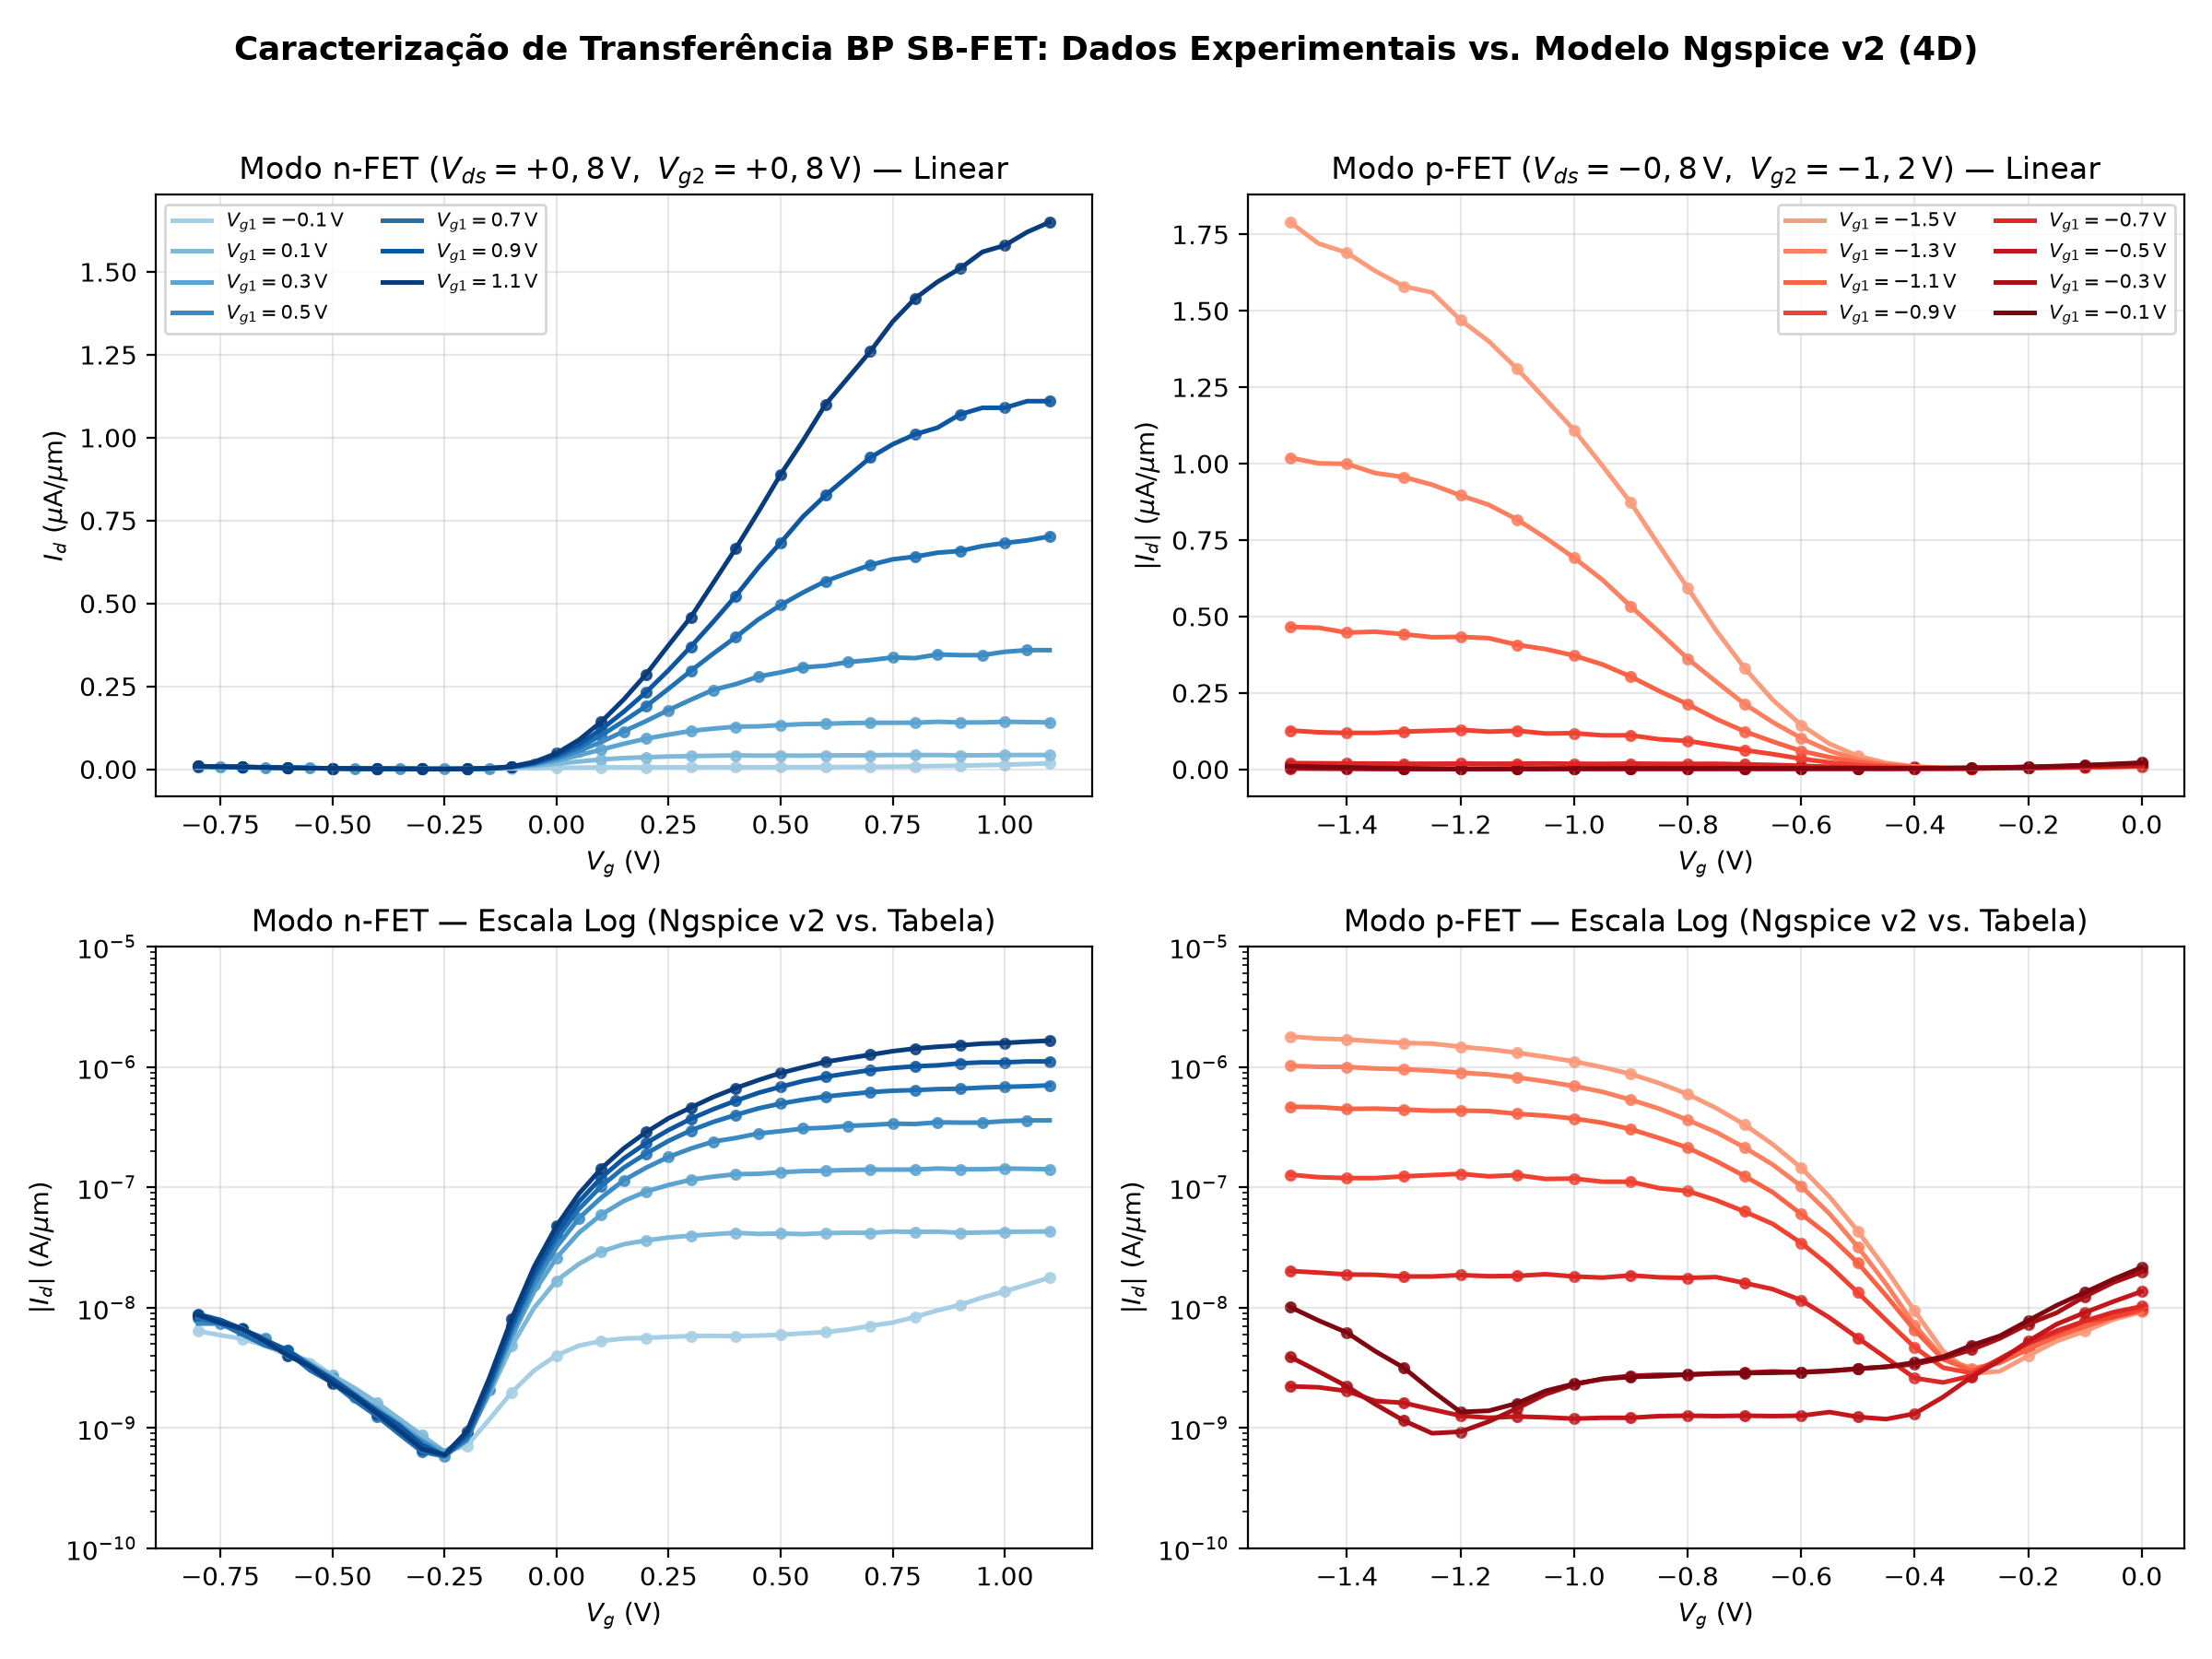
\includegraphics[width=0.92\textwidth]{m00_transfer_NP_log_lin.png}
\caption{Linear and logarithmic transfer curves ($I_d \times V_g$) simulated in \texttt{ngspice-47} against experimental data points for \textit{n-FET} and \textit{p-FET} modes.}
\label{fig:m00_transfer}
\end{figure}

\begin{figure}[htbp]
\centering
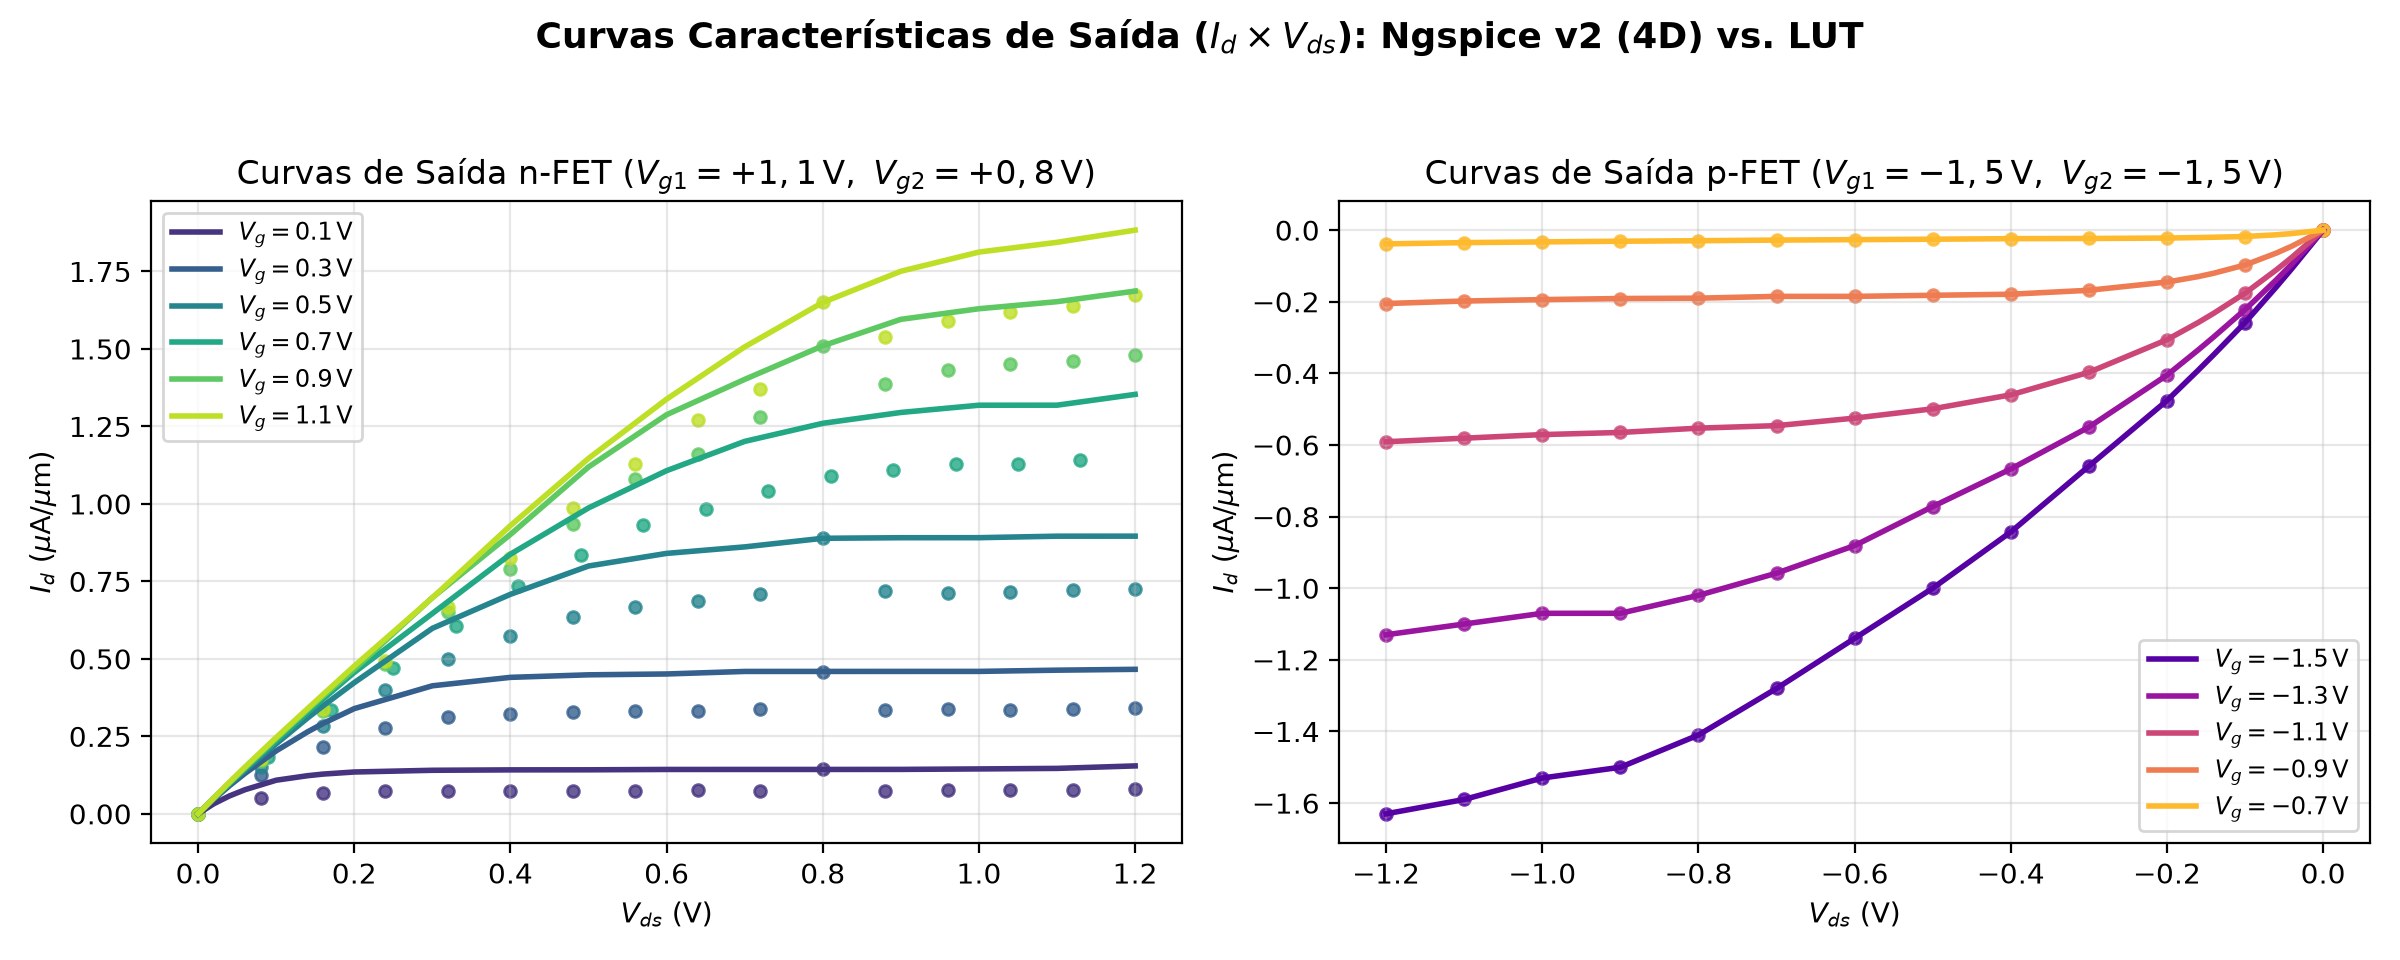
\includegraphics[width=0.92\textwidth]{m00_output_NP.png}
\caption{Output characteristic families ($I_d \times V_{ds}$) in \textit{n-FET} ($V_{ds}>0$) and \textit{p-FET} ($V_{ds}<0$, $V_{g2}=-1.5\ \text{V}$) regimes capturing gate-dependent triode-to-saturation transitions.}
\label{fig:m00_output}
\end{figure}

\begin{figure}[htbp]
\centering
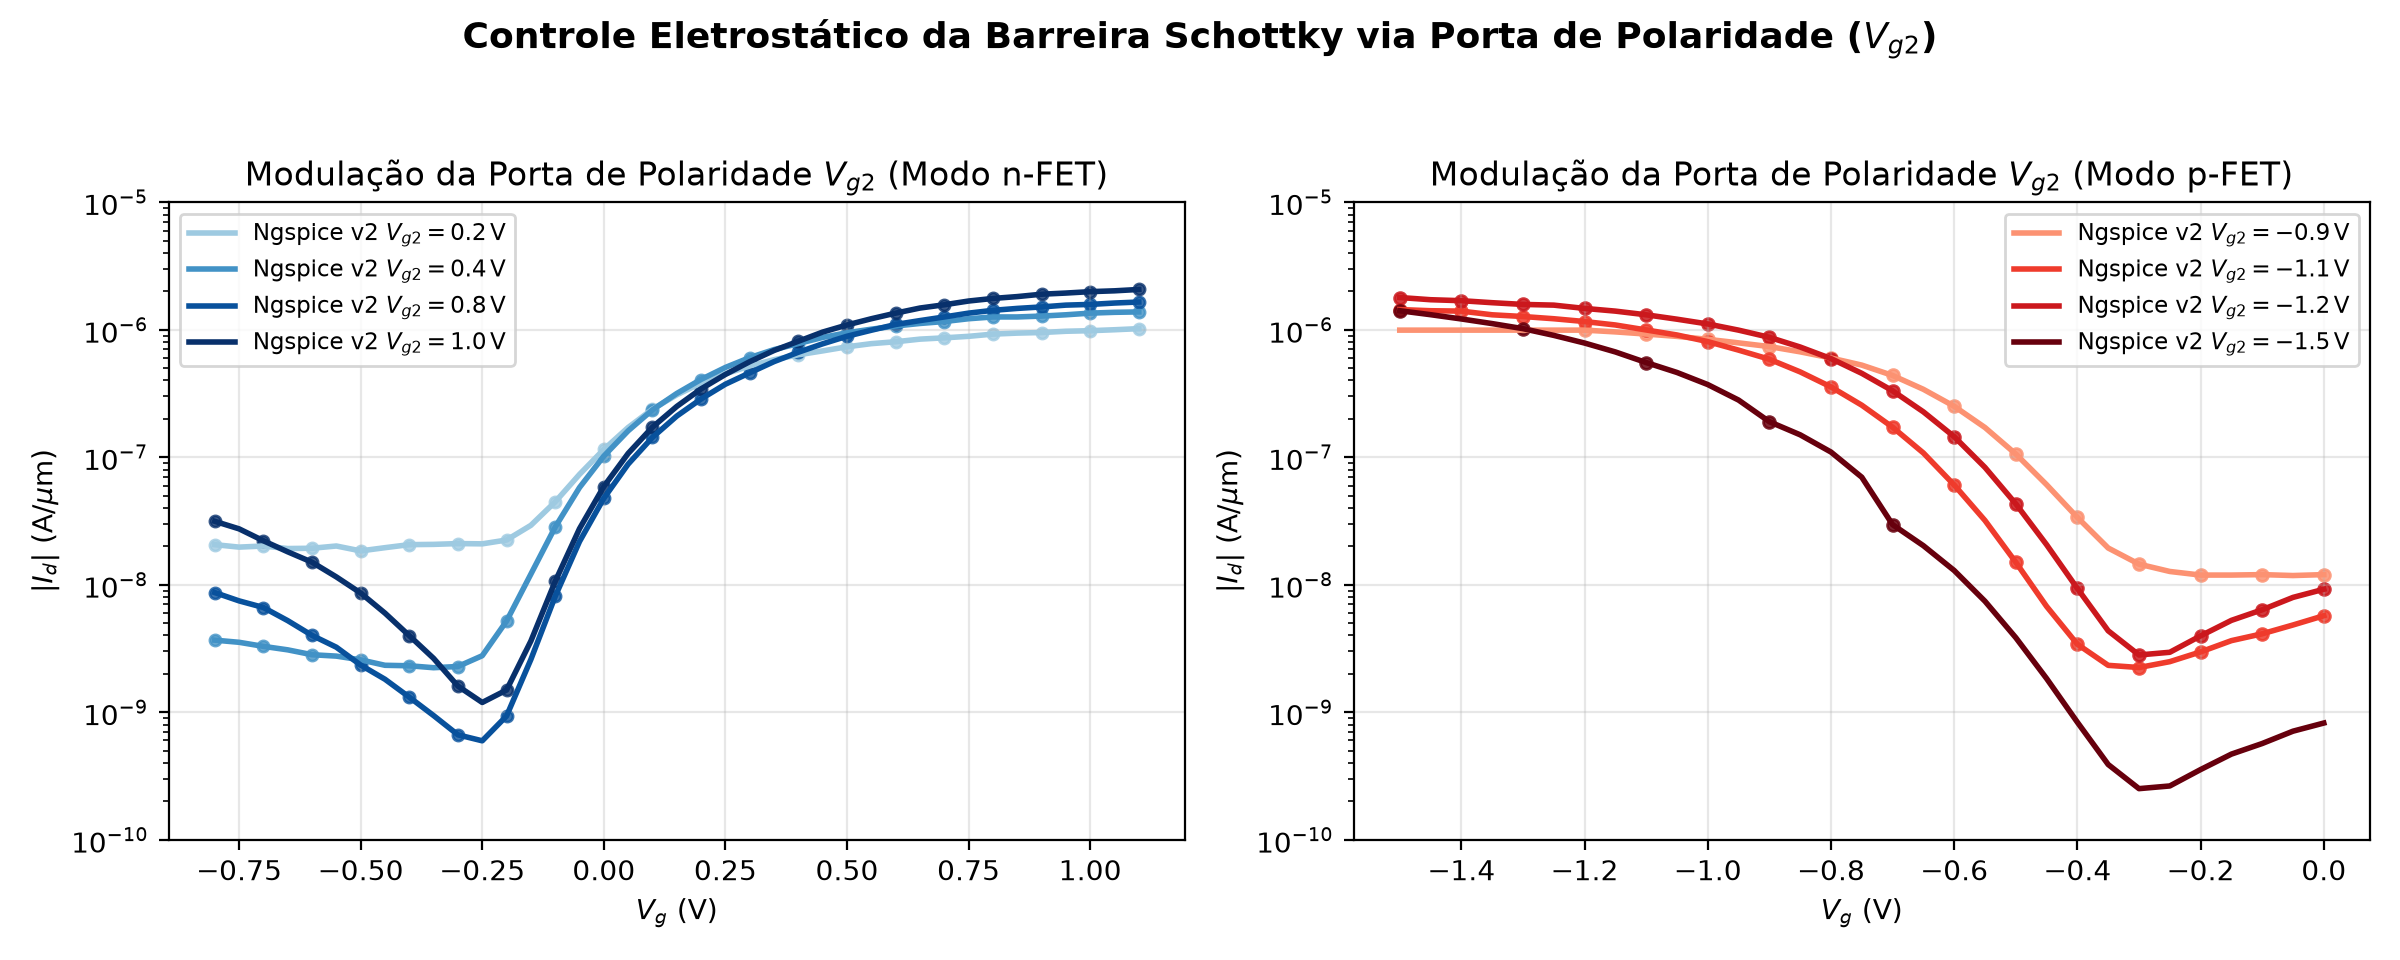
\includegraphics[width=0.92\textwidth]{m00_efeito_porta_polaridade.png}
\caption{Electrostatic modulation of channel current by the polarity gate $V_{g2}$ in \textit{n-FET} and \textit{p-FET} modes, highlighting the flat-band shift at $V_{g2}=-1.5\ \text{V}$.}
\label{fig:m00_pg}
\end{figure}

\begin{figure}[htbp]
\centering
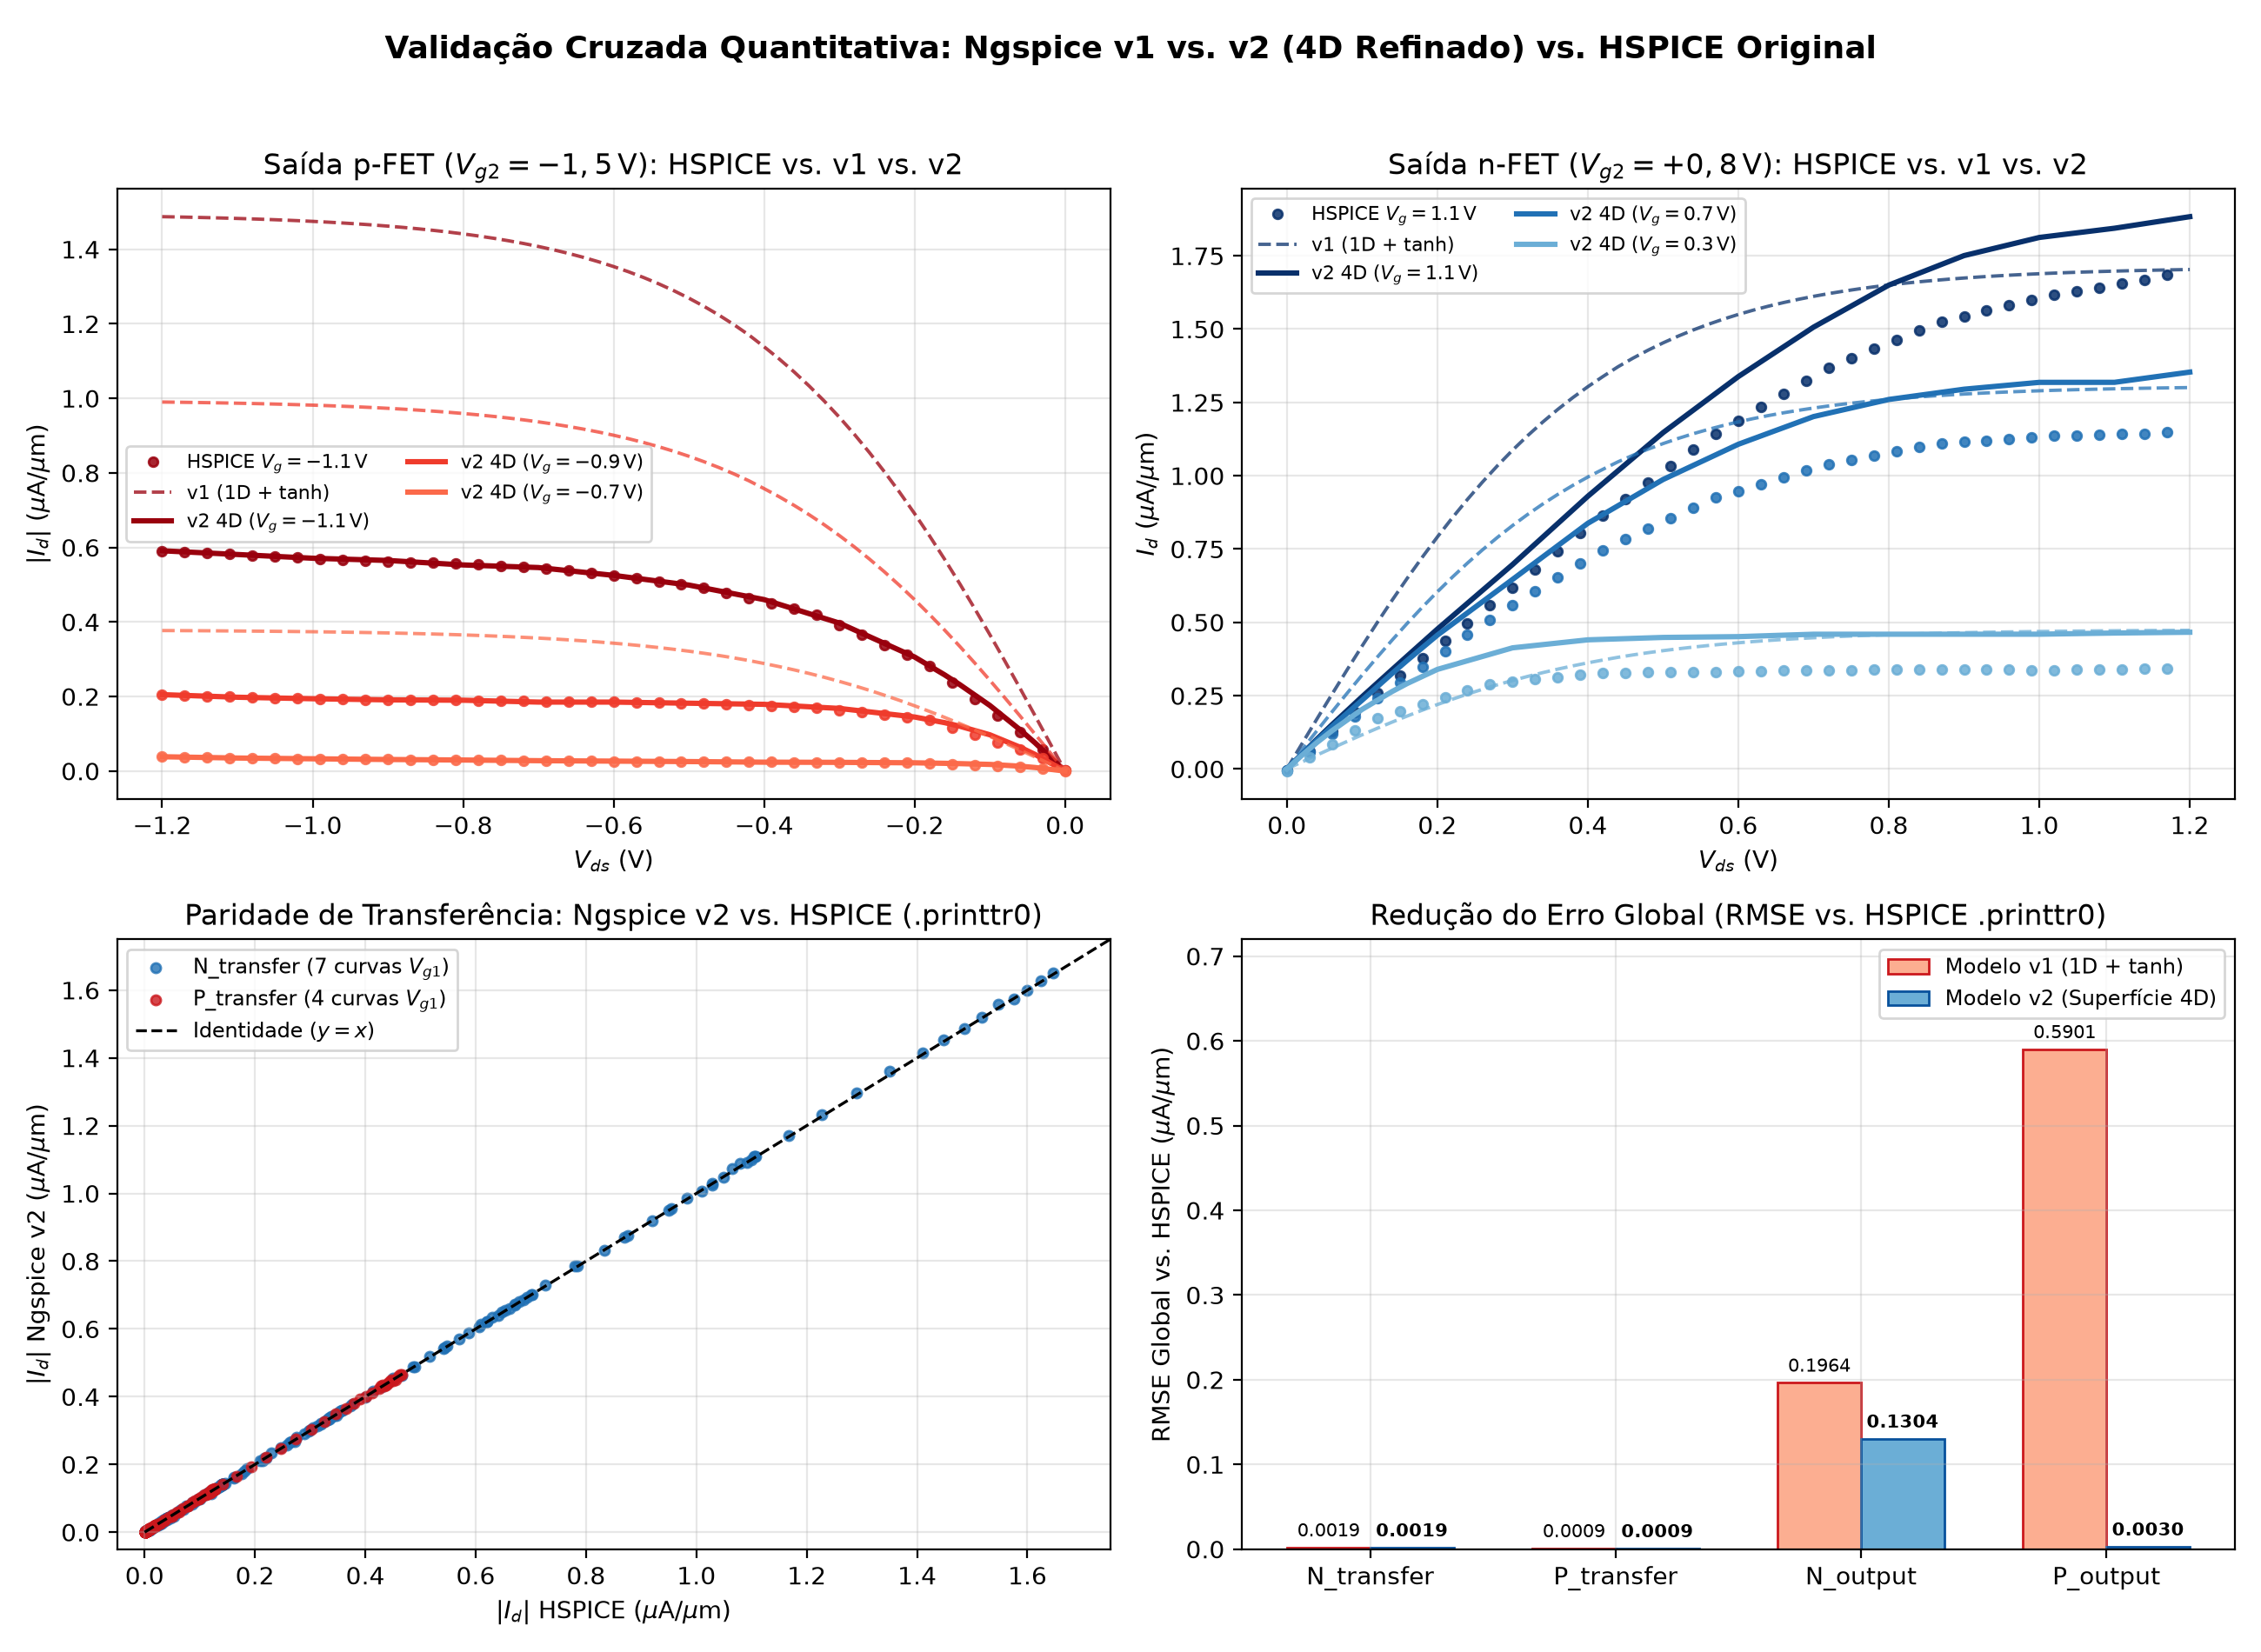
\includegraphics[width=0.92\textwidth]{m00_validacao_cruzada_hspice.png}
\caption{Quantitative cross-validation comparing the preliminary model (\texttt{v1}), the refined 4D model (\texttt{v2}) in \texttt{ngspice-47}, and the reference Synopsys HSPICE \texttt{.printtr0} traces.}
\label{fig:m00_hspice}
\end{figure}

\subsection{Ultra-Low-Voltage Complementary Inverter}\label{sec:res_inverter}

Static performance metrics of the complementary BP SB-FET inverter from $V_{DD} = 1.0\ \text{V}$ down to $0.2\ \text{V}$ are compiled in Table~\ref{tab:inverter_vtc}. Without $V_{fb}$ compensation (direct coupling), threshold misalignment between the \textit{p-FET} and \textit{n-FET} branches shifts the switching threshold $V_M$ toward $0\ \text{V}$, collapsing inverter functionality for $V_{DD} \le 0.4\ \text{V}$ ($2.77\%$ swing and $|A_v|_{\max} = 0.37$ at $0.4\ \text{V}$; $1.27\%$ swing and $0.06$ gain at $0.2\ \text{V}$).

\begin{table}[htbp]
\centering
\caption{Static metrics of the complementary BP SB-FET inverter under $V_{DD}$ scaling ($1.0\ \text{V}$ to $0.2\ \text{V}$).}
\label{tab:inverter_vtc}
\resizebox{\textwidth}{!}{%
\begin{tabular}{l c c c c c c c c}
\toprule
\textbf{Configuration} & $V_{DD}$ (V) & $V_{\mathrm{out}}(0)$ (V) & $V_{\mathrm{out}}(V_{DD})$ (V) & \textbf{Swing (\%)} & $V_M$ (V) & $|A_v|_{\max}$ & $NM_L$ (V) & $NM_H$ (V) \\
\midrule
Direct (No $V_{fb}$ comp.) & $1.0$ & $0.991$ & $0.004$ & $98.67\%$ & $0.278$ & $22.03$ & $0.096$ & $0.564$ \\
Direct (No $V_{fb}$ comp.) & $0.8$ & $0.788$ & $0.004$ & $98.12\%$ & $0.162$ & $39.32$ & $0.034$ & $0.537$ \\
Direct (No $V_{fb}$ comp.) & $0.6$ & $0.559$ & $0.003$ & $92.68\%$ & $0.066$ & $37.24$ & $0.000$ & $0.475$ \\
Direct (No $V_{fb}$ comp.) & $0.4$ & $0.014$ & $0.003$ & $2.77\%$  & $0.010$ & $0.37$  & $0.000$ & $0.000$ \\
Direct (No $V_{fb}$ comp.) & $0.2$ & $0.005$ & $0.003$ & $1.27\%$  & $0.006$ & $0.06$  & $0.000$ & $0.000$ \\
\midrule
Compensated ($V_{fb}$ aligned) & $1.0$ & $0.999$ & $0.003$ & $99.63\%$ & $0.540$ & $54.69$ & $0.461$ & $0.373$ \\
Compensated ($V_{fb}$ aligned) & $0.8$ & $0.800$ & $0.002$ & $99.75\%$ & $0.438$ & $50.84$ & $0.362$ & $0.278$ \\
Compensated ($V_{fb}$ aligned) & $0.6$ & $0.600$ & $0.001$ & $99.80\%$ & $0.336$ & $38.18$ & $0.266$ & $0.178$ \\
Compensated ($V_{fb}$ aligned) & $0.4$ & $0.400$ & $0.003$ & $99.29\%$ & $0.234$ & $12.71$ & $0.172$ & $0.076$ \\
Compensated ($V_{fb}$ aligned) & $0.2$ & $0.198$ & $0.018$ & $89.75\%$ & $0.126$ & $2.71$  & $0.080$ & $0.000$ \\
\bottomrule
\end{tabular}}
\end{table}

With electrostatic $V_{fb}$ alignment, $V_M$ centers near $V_{DD}/2$ (Figure~\ref{fig:m01_vtc}), sustaining over $99.2\%$ output swing down to $0.4\ \text{V}$ and reaching peak voltage gains of $|A_v|_{\max} = 54.69$ ($1.0\ \text{V}$) and $38.18$ ($0.6\ \text{V}$). Even at the extreme ultra-low-voltage regime ($V_{DD} = 0.2\ \text{V}$), the inverter maintains $89.75\%$ rail-to-rail swing and differential gain $2.71 > 1$, satisfying the criterion for logic regeneration. In transient switching under $C_{\mathrm{load}} = 0.5\ \text{fF}$ (Figure~\ref{fig:m01_tran}), transitions complete on the nanosecond scale with nanoampere static leakage and dynamic current peaks of $1.28\ \mu\text{A}$ at $1.0\ \text{V}$ and $0.73\ \mu\text{A}$ at $0.6\ \text{V}$.

\begin{figure}[htbp]
\centering
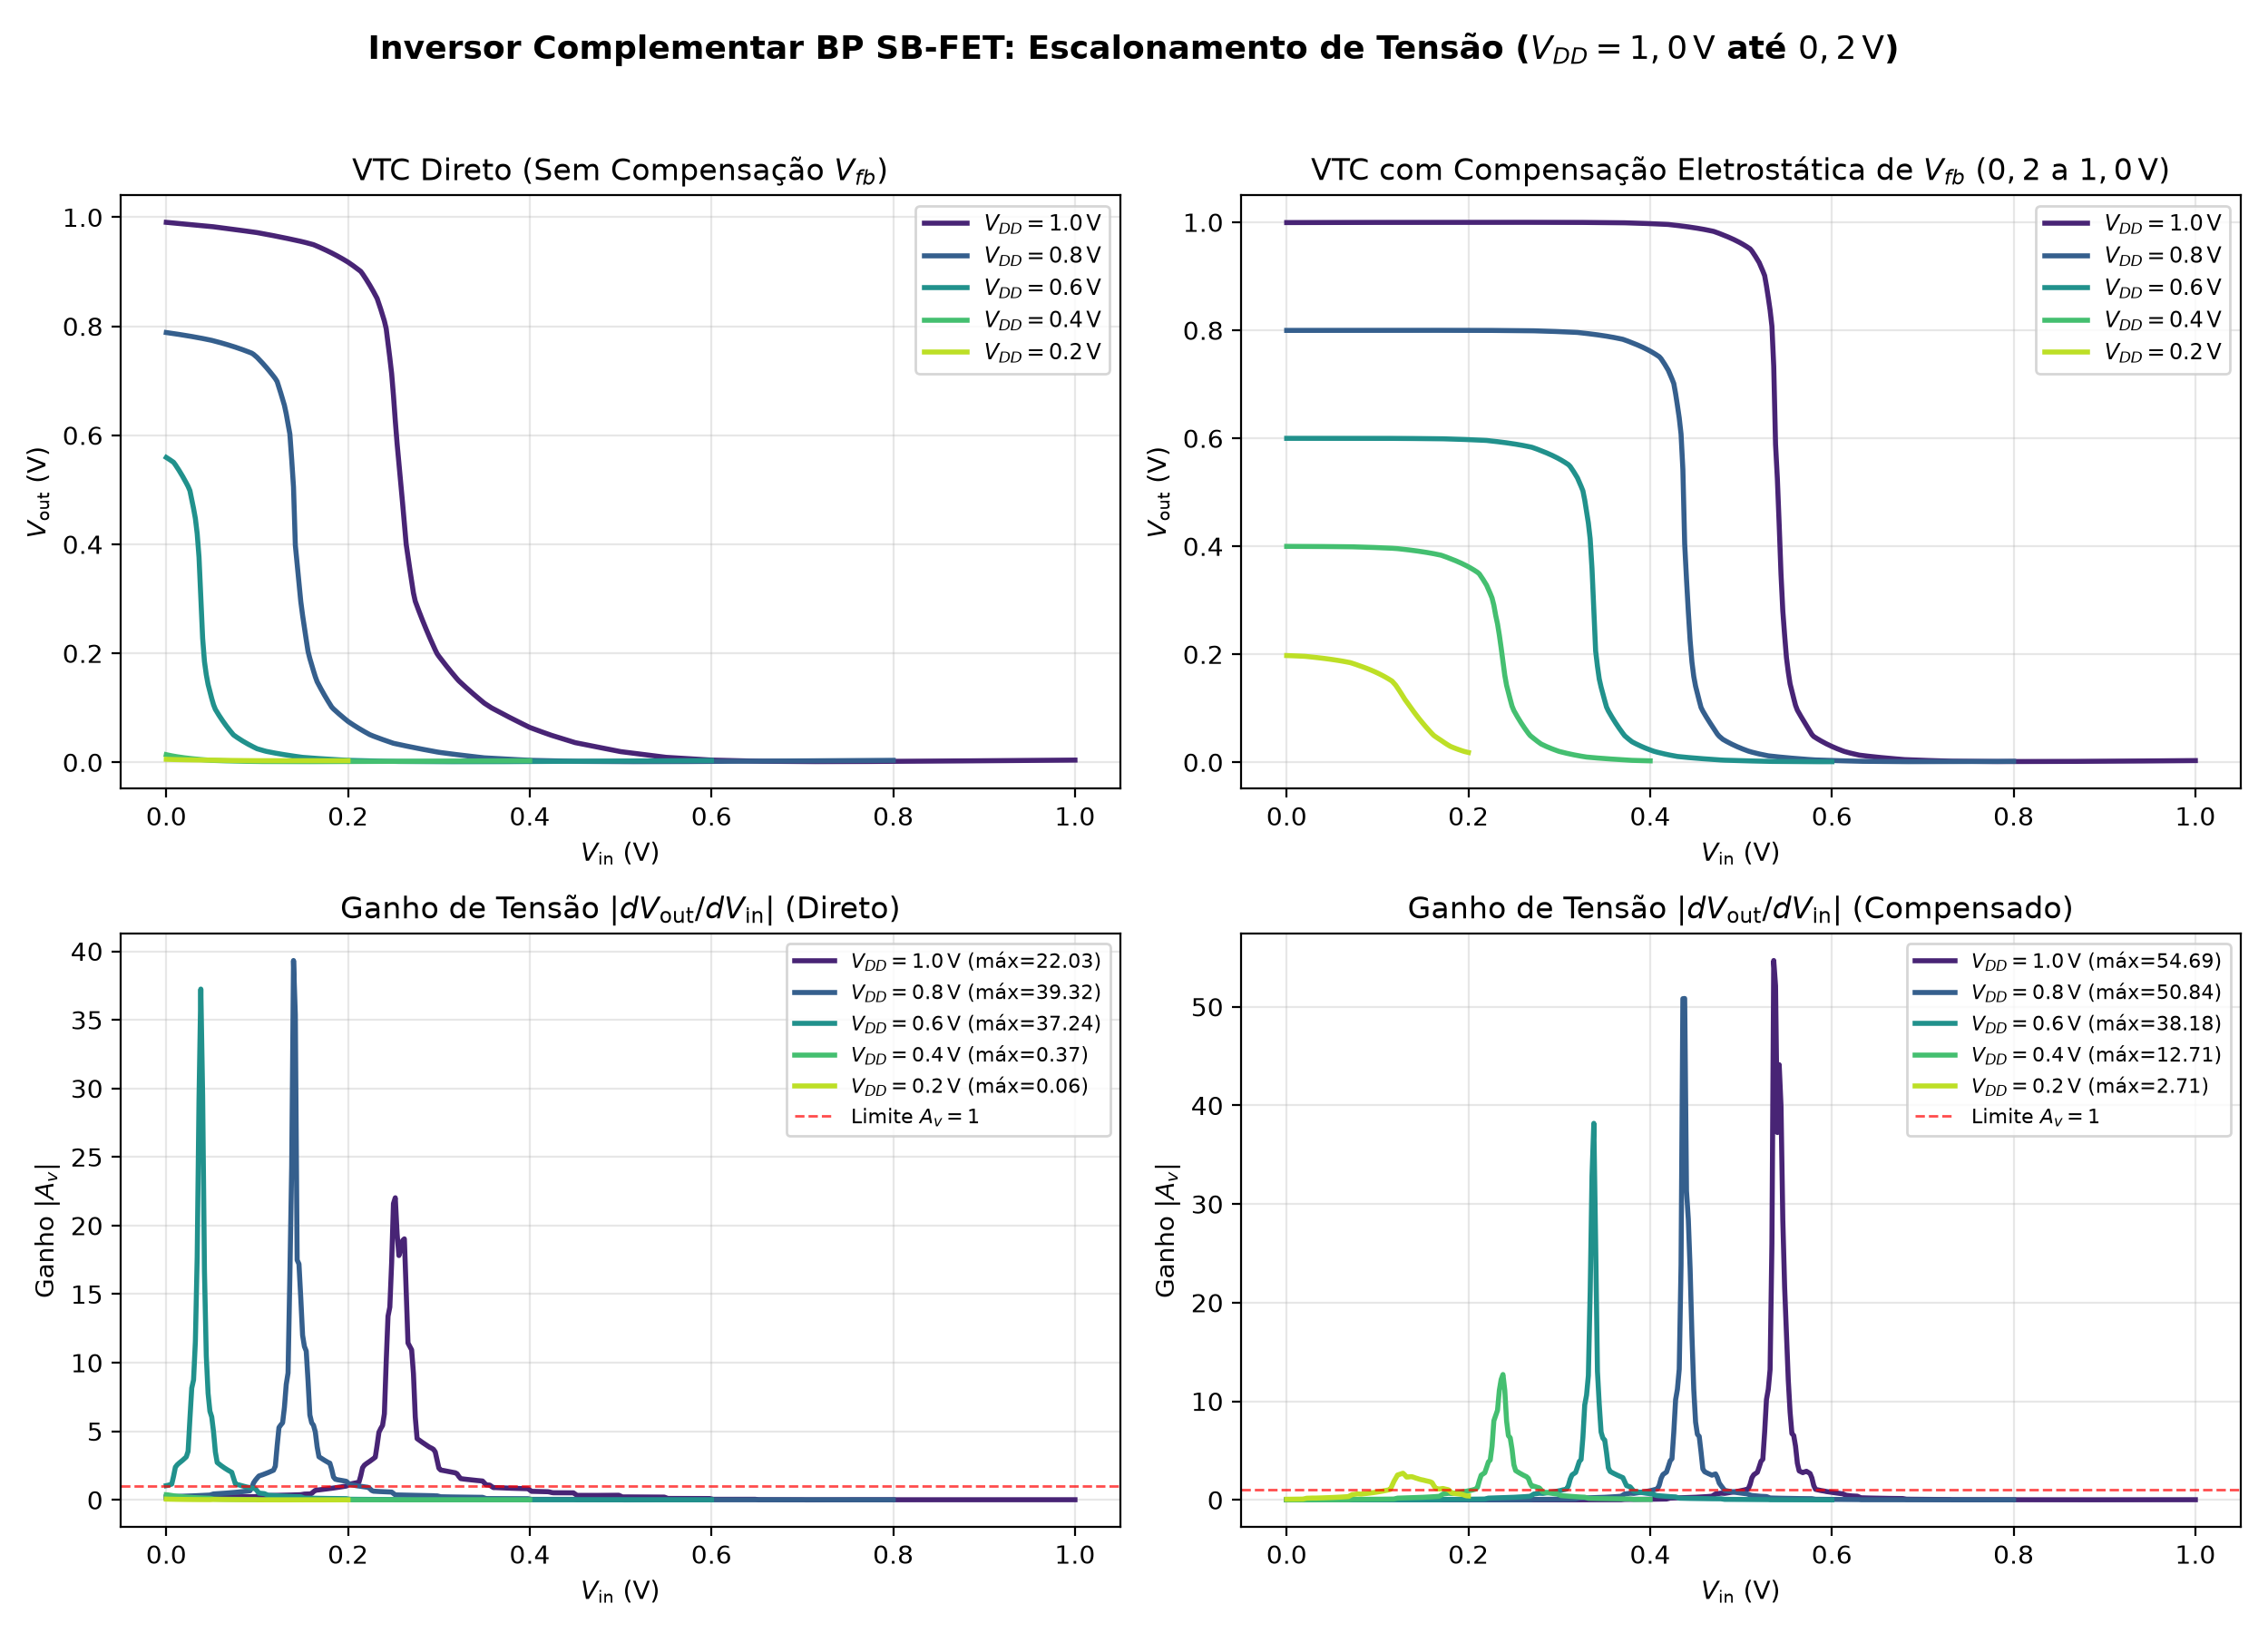
\includegraphics[width=0.92\textwidth]{m01_inversor_vtc_ganho.png}
\caption{Voltage transfer characteristics (VTC) and differential gain $|dV_{\mathrm{out}}/dV_{\mathrm{in}}|$ of the BP SB-FET inverter without compensation (left) and with $V_{fb}$ alignment (right) from $1.0\ \text{V}$ to $0.2\ \text{V}$.}
\label{fig:m01_vtc}
\end{figure}

\begin{figure}[htbp]
\centering
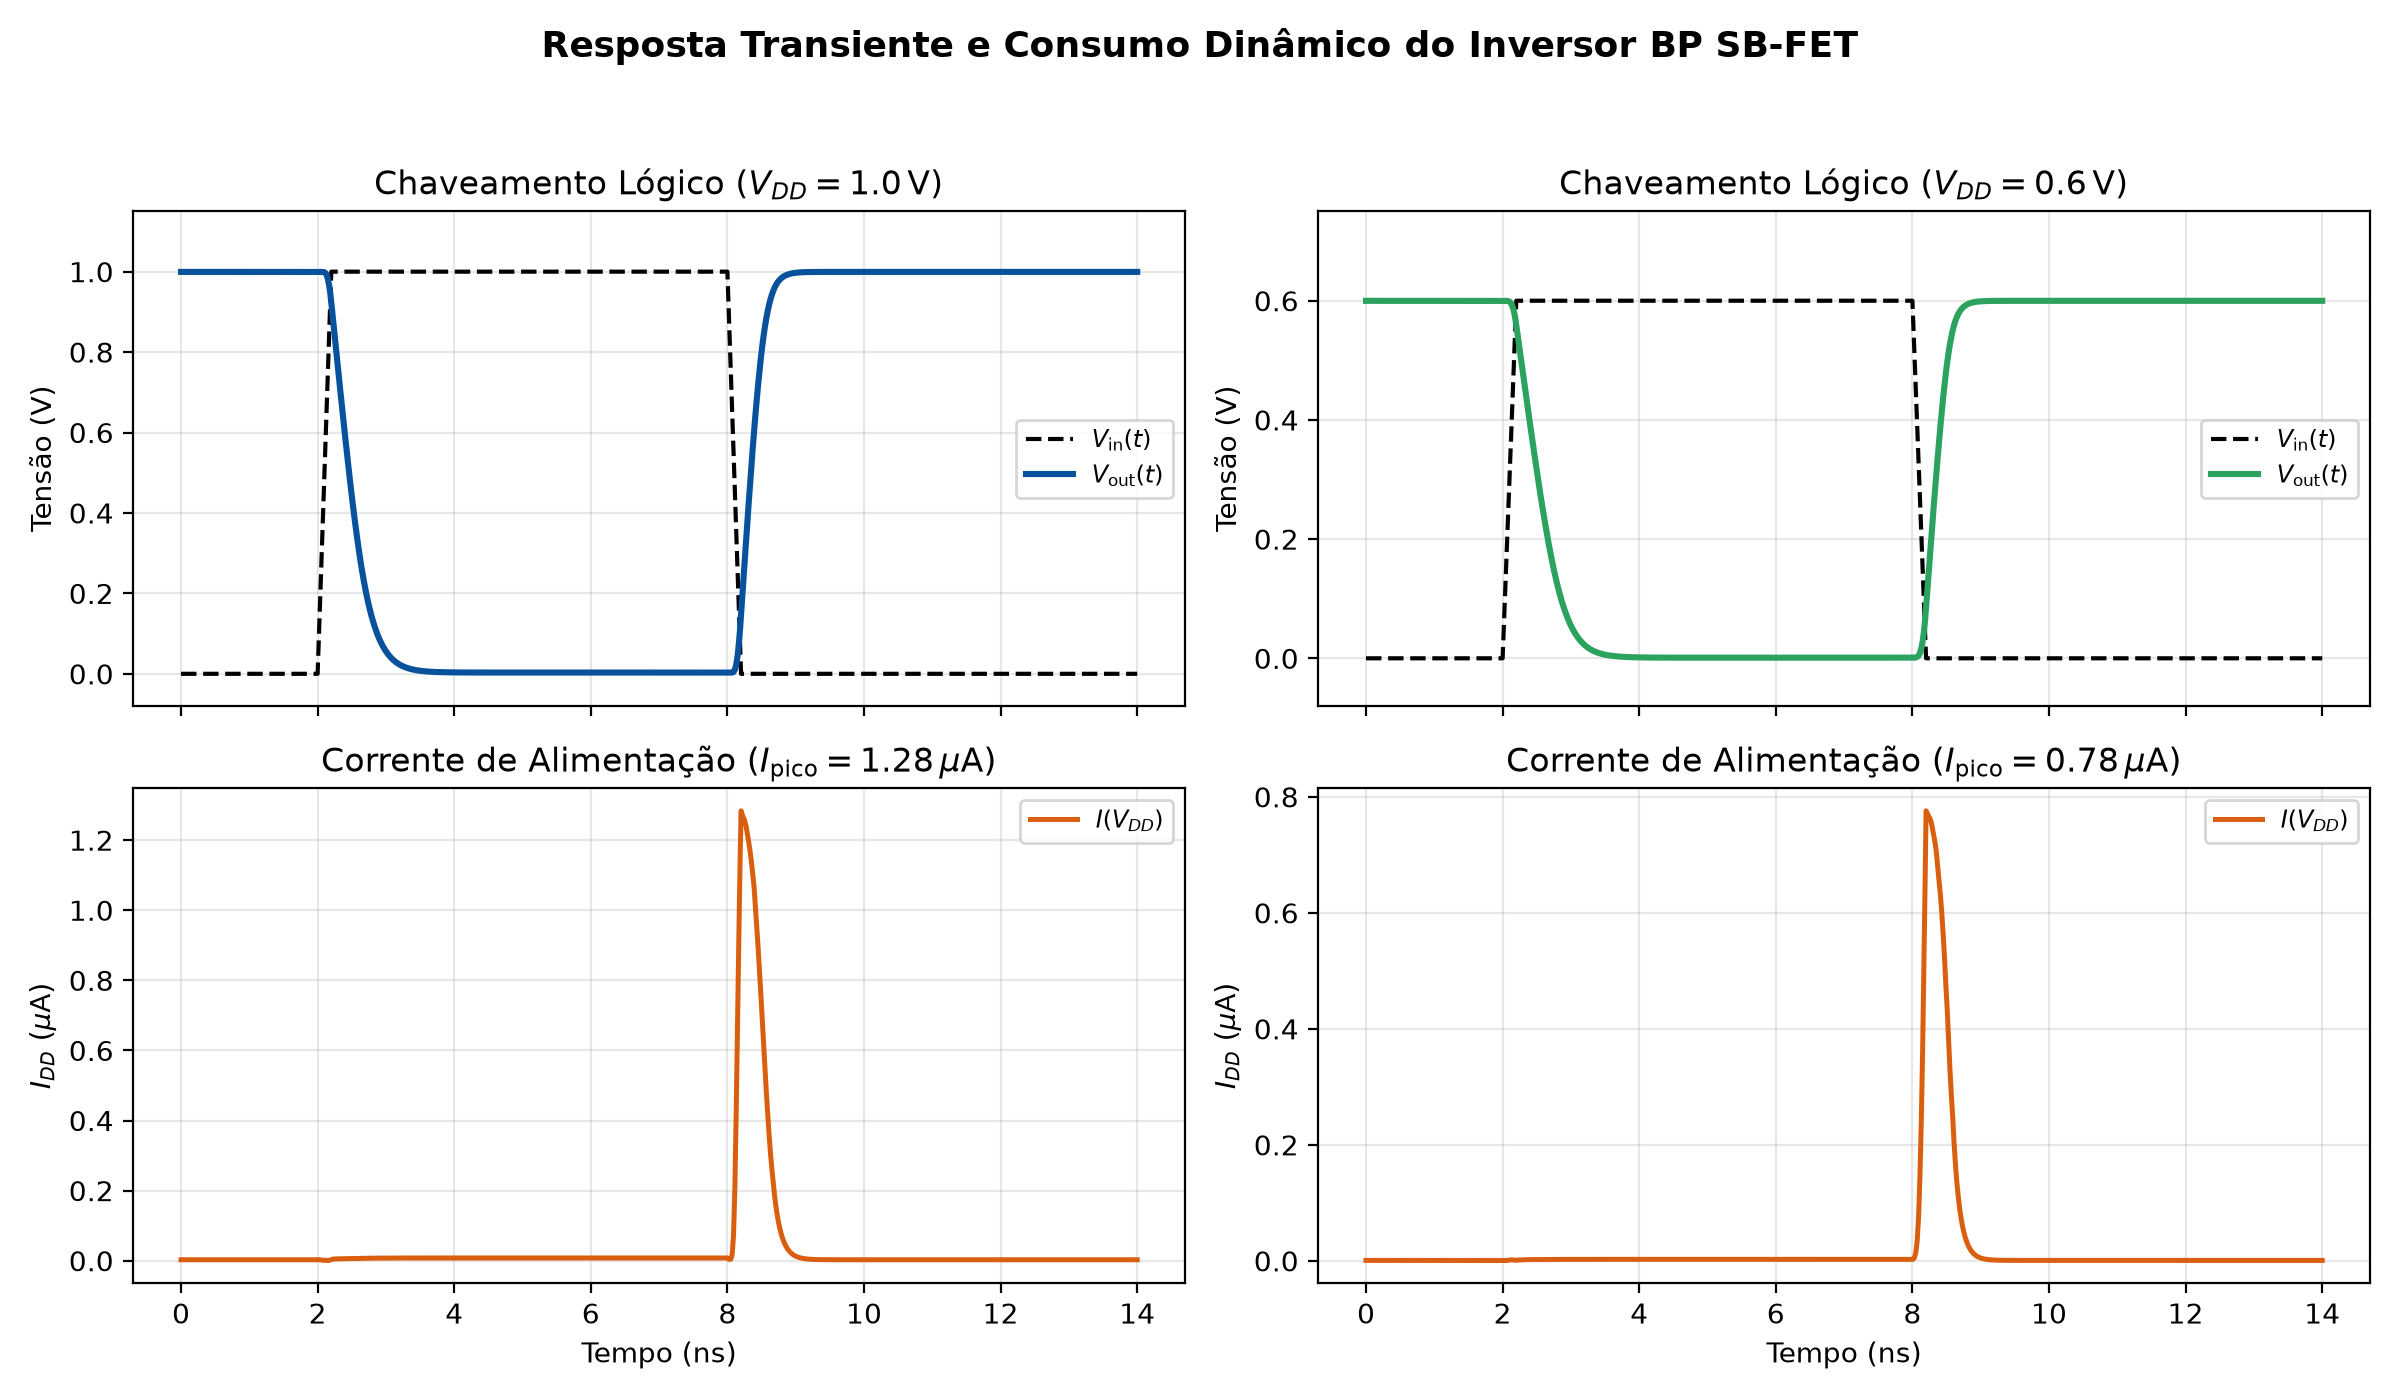
\includegraphics[width=0.90\textwidth]{m01_inversor_transiente.png}
\caption{Transient switching response ($C_{\mathrm{load}} = 0.5\ \text{fF}$) and dynamic supply current peaks $I(V_{DD})$ of the compensated inverter at $V_{DD} = 1.0\ \text{V}$ and $0.6\ \text{V}$.}
\label{fig:m01_tran}
\end{figure}

\subsection{Dynamic Polymorphic Logic Gates (\texttt{NAND}/\texttt{NOR} and \texttt{XOR}/\texttt{XNOR})}\label{sec:res_poly}

The $40\ \text{ns}$ transient simulations verified $100\%$ Boolean accuracy ($16/16$ input-key combinations) across both 4-transistor polymorphic primitives with zero transistor overhead, as detailed in Table~\ref{tab:polymorphic_gates}. In the \texttt{NAND}/\texttt{NOR} cell ($V_{DD}=0.8\ \text{V}$), logic \texttt{'1'} outputs range between $0.701\ \text{V}$ and $0.790\ \text{V}$, while logic \texttt{'0'} outputs remain below $0.013\ \text{V}$. In the \texttt{XOR}/\texttt{XNOR} bridge ($V_{DD}=1.5\ \text{V}$, $V_{\mathrm{in}}=1.1\ \text{V}$), all \texttt{'1'} states settle at $1.465\ \text{V}$ and all \texttt{'0'} states settle at $0.002\ \text{V}$.

\begin{table}[htbp]
\centering
\caption{Electrical truth table and peak currents measured in \texttt{ngspice-47} for the 4T polymorphic gates.}
\label{tab:polymorphic_gates}
\footnotesize
\begin{tabular}{l c c c c c c c}
\toprule
\textbf{Gate ($V_{DD}$)} & \textbf{Key} & \textbf{Function} & $(A,B)$ & $V_{\mathrm{out}}$ (V) & \textbf{Meas.\ Bit} & \textbf{Exp.\ Bit} & $I_{\mathrm{peak}}$ ($\mu\text{A}$) \\
\midrule
\texttt{NAND}/\texttt{NOR} ($0.8\ \text{V}$) & $\text{Key}=0$ & \texttt{NAND} & \texttt{00} & $0.790$ & \texttt{1} & \texttt{1} & $0.041$ \\
\texttt{NAND}/\texttt{NOR} ($0.8\ \text{V}$) & $\text{Key}=0$ & \texttt{NAND} & \texttt{01} & $0.762$ & \texttt{1} & \texttt{1} & $0.182$ \\
\texttt{NAND}/\texttt{NOR} ($0.8\ \text{V}$) & $\text{Key}=0$ & \texttt{NAND} & \texttt{10} & $0.769$ & \texttt{1} & \texttt{1} & $0.390$ \\
\texttt{NAND}/\texttt{NOR} ($0.8\ \text{V}$) & $\text{Key}=0$ & \texttt{NAND} & \texttt{11} & $0.013$ & \texttt{0} & \texttt{0} & $0.589$ \\
\texttt{NAND}/\texttt{NOR} ($0.8\ \text{V}$) & $\text{Key}=1$ & \texttt{NOR}  & \texttt{00} & $0.701$ & \texttt{1} & \texttt{1} & $0.213$ \\
\texttt{NAND}/\texttt{NOR} ($0.8\ \text{V}$) & $\text{Key}=1$ & \texttt{NOR}  & \texttt{01} & $0.001$ & \texttt{0} & \texttt{0} & $0.716$ \\
\texttt{NAND}/\texttt{NOR} ($0.8\ \text{V}$) & $\text{Key}=1$ & \texttt{NOR}  & \texttt{10} & $0.004$ & \texttt{0} & \texttt{0} & $0.092$ \\
\texttt{NAND}/\texttt{NOR} ($0.8\ \text{V}$) & $\text{Key}=1$ & \texttt{NOR}  & \texttt{11} & $0.001$ & \texttt{0} & \texttt{0} & $0.006$ \\
\midrule
\texttt{XOR}/\texttt{XNOR} ($1.5\ \text{V}$) & $\text{Key}=0$ & \texttt{XOR}  & \texttt{00} & $0.002$ & \texttt{0} & \texttt{0} & $0.004$ \\
\texttt{XOR}/\texttt{XNOR} ($1.5\ \text{V}$) & $\text{Key}=0$ & \texttt{XOR}  & \texttt{01} & $1.465$ & \texttt{1} & \texttt{1} & $1.691$ \\
\texttt{XOR}/\texttt{XNOR} ($1.5\ \text{V}$) & $\text{Key}=0$ & \texttt{XOR}  & \texttt{10} & $1.465$ & \texttt{1} & \texttt{1} & $0.366$ \\
\texttt{XOR}/\texttt{XNOR} ($1.5\ \text{V}$) & $\text{Key}=0$ & \texttt{XOR}  & \texttt{11} & $0.002$ & \texttt{0} & \texttt{0} & $1.903$ \\
\texttt{XOR}/\texttt{XNOR} ($1.5\ \text{V}$) & $\text{Key}=1$ & \texttt{XNOR} & \texttt{00} & $1.465$ & \texttt{1} & \texttt{1} & $1.699$ \\
\texttt{XOR}/\texttt{XNOR} ($1.5\ \text{V}$) & $\text{Key}=1$ & \texttt{XNOR} & \texttt{01} & $0.002$ & \texttt{0} & \texttt{0} & $1.908$ \\
\texttt{XOR}/\texttt{XNOR} ($1.5\ \text{V}$) & $\text{Key}=1$ & \texttt{XNOR} & \texttt{10} & $0.002$ & \texttt{0} & \texttt{0} & $0.032$ \\
\texttt{XOR}/\texttt{XNOR} ($1.5\ \text{V}$) & $\text{Key}=1$ & \texttt{XNOR} & \texttt{11} & $1.465$ & \texttt{1} & \texttt{1} & $1.691$ \\
\bottomrule
\end{tabular}
\end{table}

Figures~\ref{fig:m02_nand_nor} and \ref{fig:m02_xor_xnor} demonstrate instantaneous functional transmutation at $t = 20\ \text{ns}$ and highlight a key structural contrast: whereas \texttt{NAND}/\texttt{NOR} displays current peaks strongly governed by which series or parallel network drives the transition, the \texttt{XOR}/\texttt{XNOR} bridge exhibits nearly identical charging ($\approx 1.69\ \mu\text{A}$) and discharging ($\approx 1.90\text{--}1.91\ \mu\text{A}$) peaks across both key configurations.

\begin{figure}[htbp]
\centering
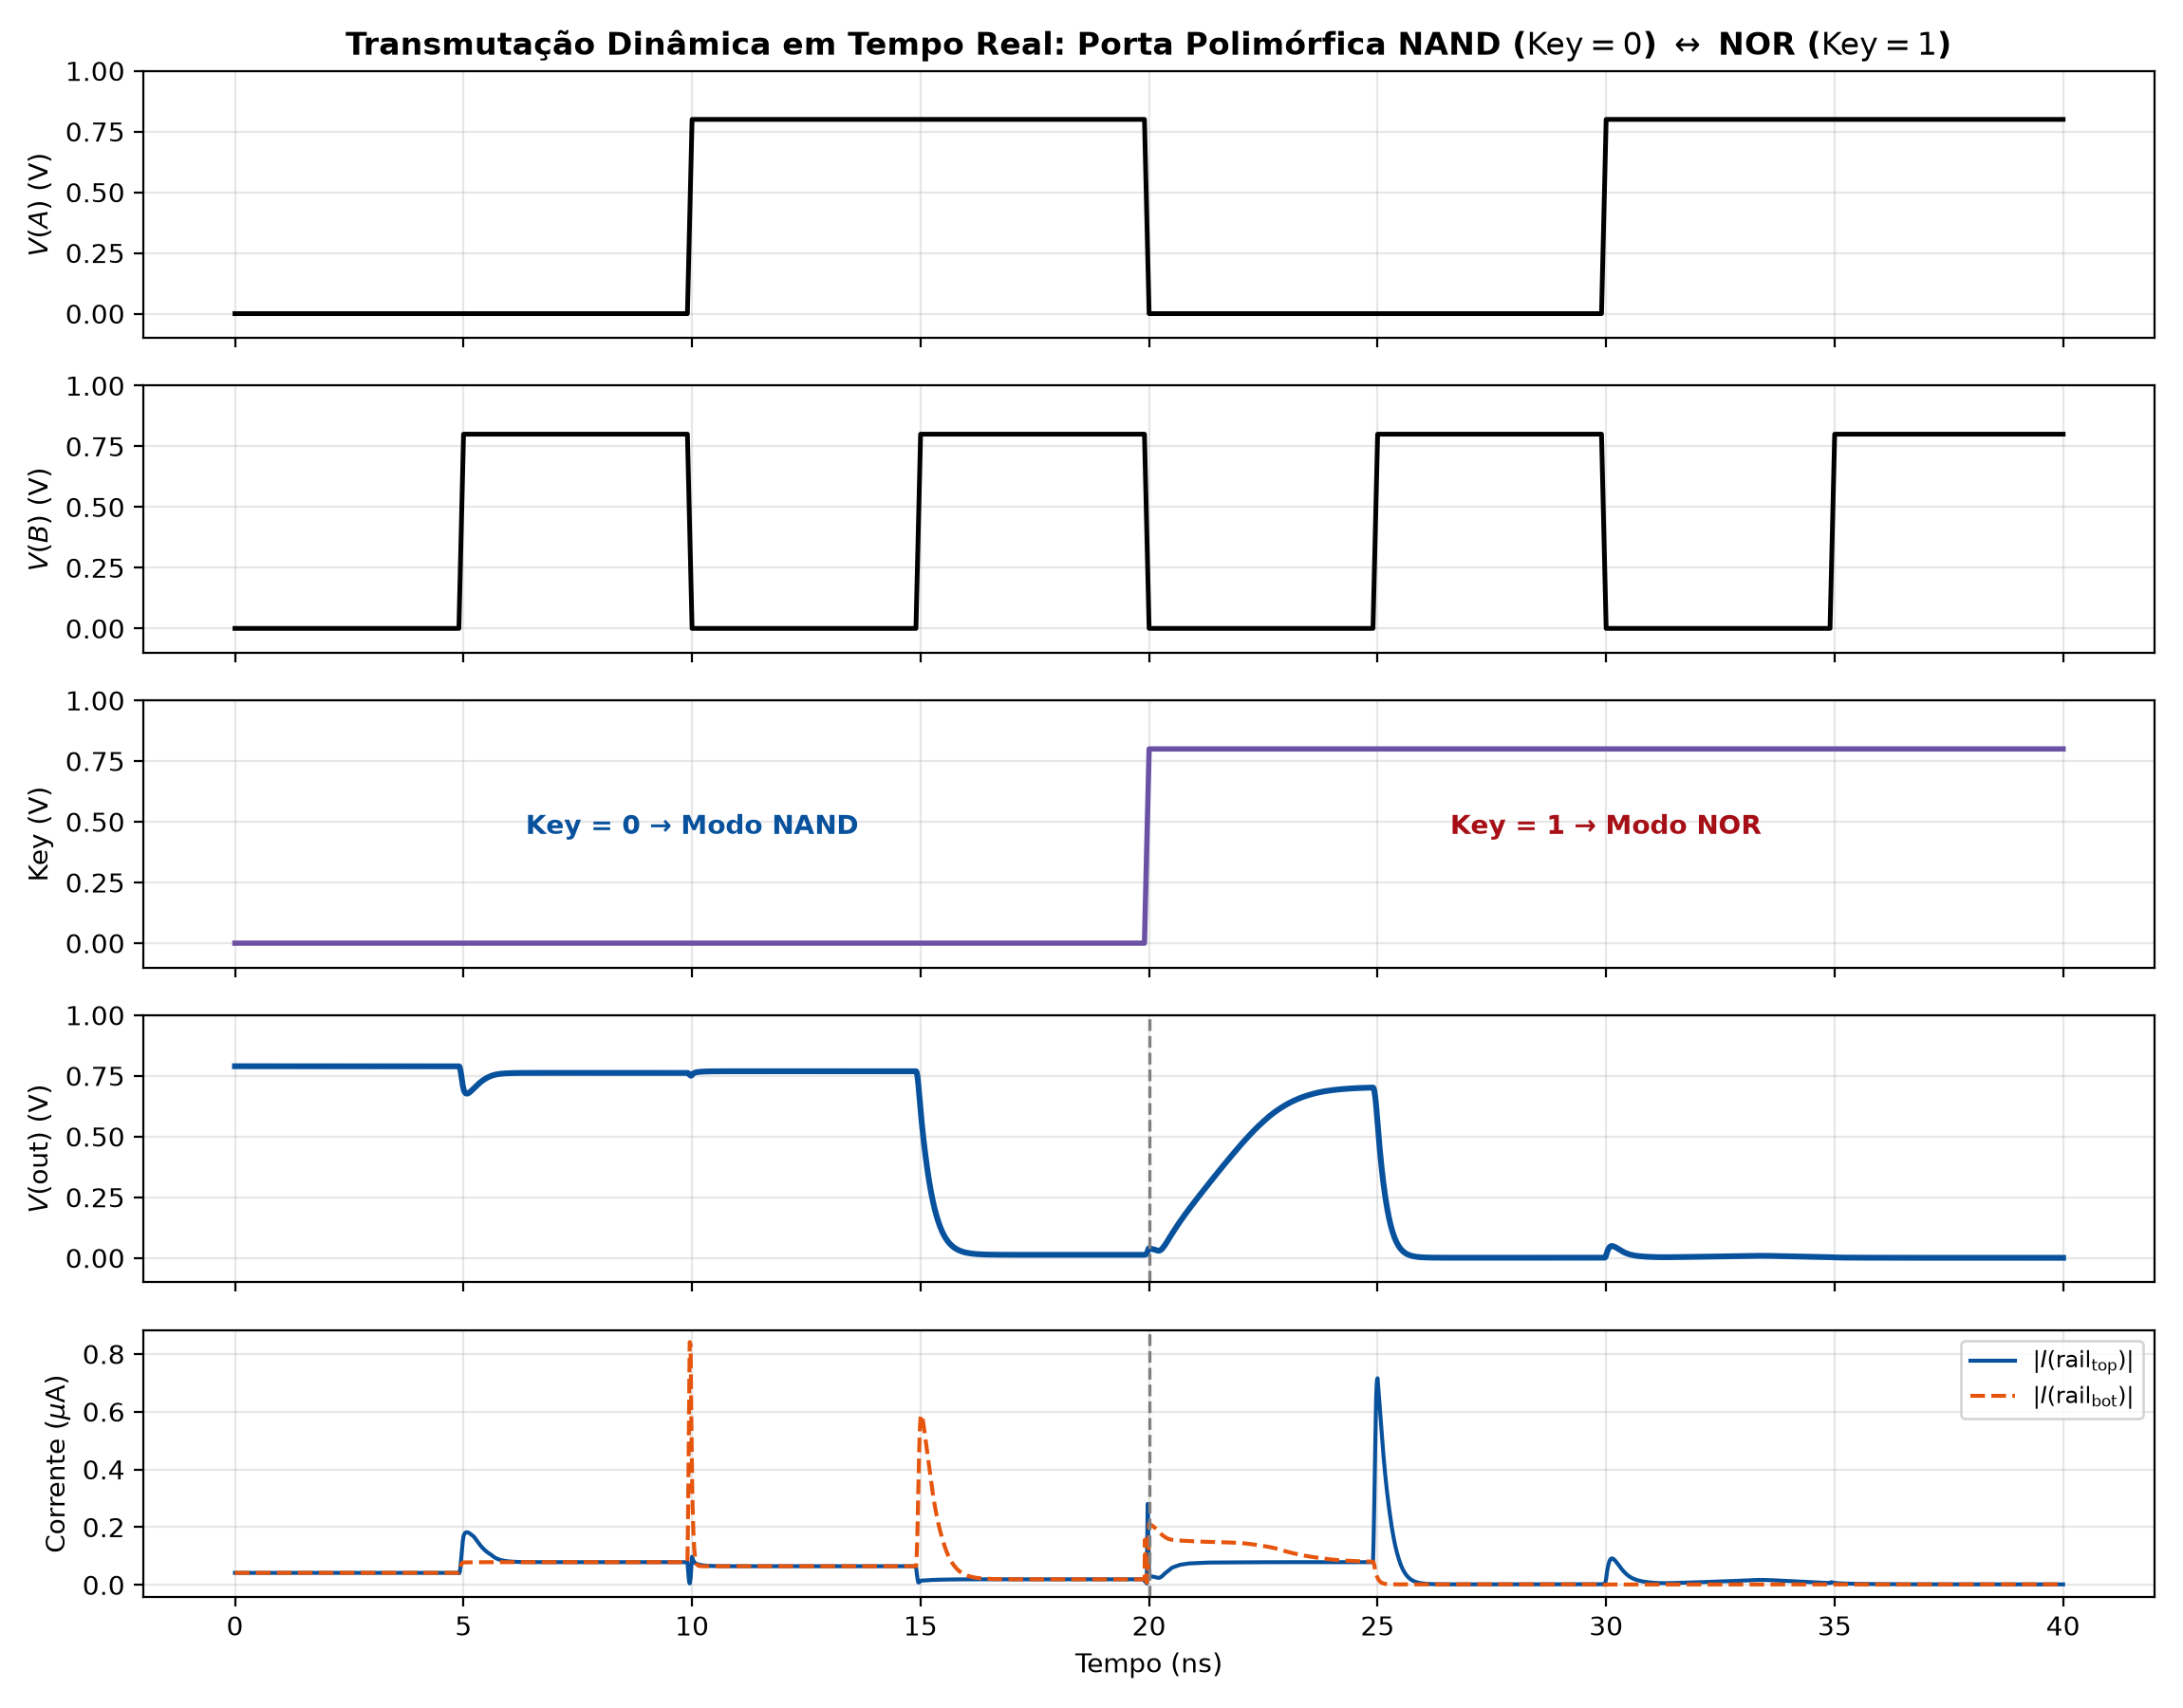
\includegraphics[width=0.90\textwidth]{m02_nand_nor_dinamico.png}
\caption{Dynamic switching \texttt{NAND} ($\text{Key}=0$) $\leftrightarrow$ \texttt{NOR} ($\text{Key}=1$) at $V_{DD} = 0.8\ \text{V}$ and its asymmetric supply current profile.}
\label{fig:m02_nand_nor}
\end{figure}

\begin{figure}[htbp]
\centering
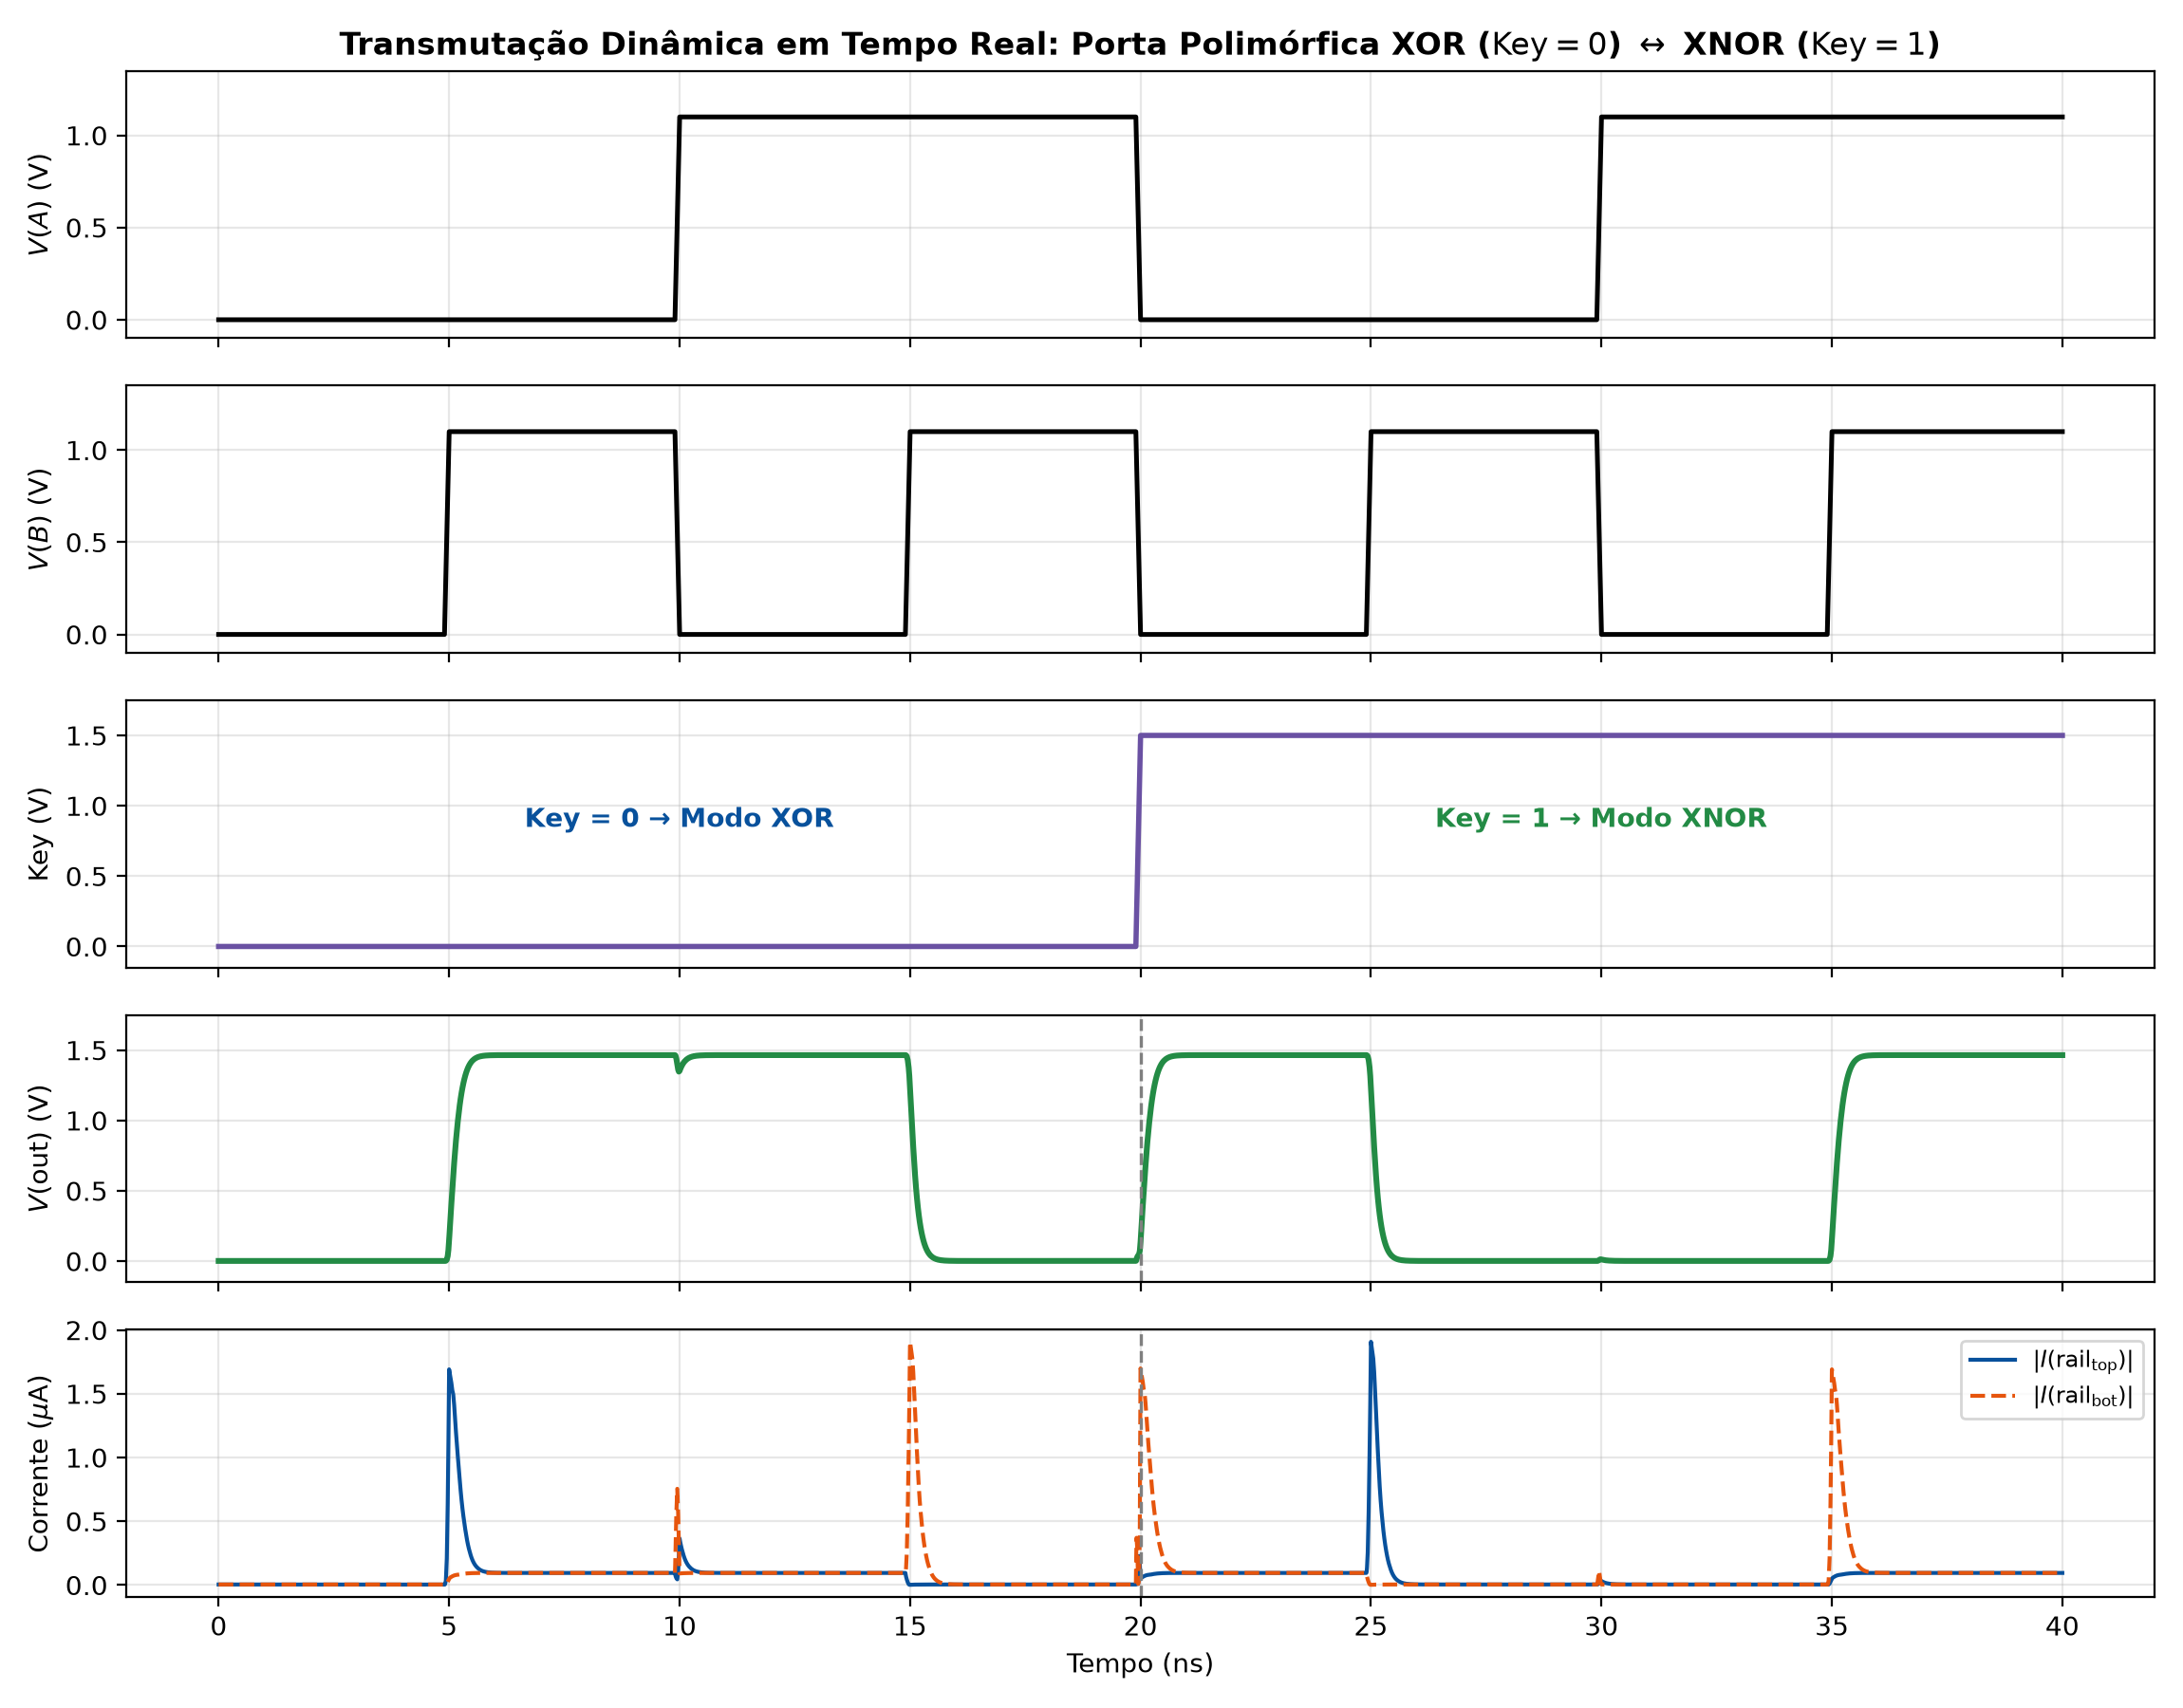
\includegraphics[width=0.90\textwidth]{m02_xor_xnor_dinamico.png}
\caption{Dynamic switching \texttt{XOR} ($\text{Key}=0$) $\leftrightarrow$ \texttt{XNOR} ($\text{Key}=1$) at $V_{DD} = 1.5\ \text{V}$ showing symmetric complementary switching current peaks.}
\label{fig:m02_xor_xnor}
\end{figure}

\subsection{Side-Channel Security (DPA), 3D Robustness, and Floating Retention}\label{sec:res_dpa_mc}

The Python port of the reference waveform datasets~\cite{wu2020reconfigurable} (Table~\ref{tab:dpa_mc_m03} and Figure~\ref{fig:m03_dpa}) confirms that the \texttt{NAND}/\texttt{NOR} family exhibits a $50.35\%$ peak current discrepancy ($2.15\ \mu\text{A}$ vs.\ $1.43\ \mu\text{A}$) and moderate temporal correlation ($r = 0.515$), whereas \texttt{XOR}/\texttt{XNOR} suppresses peak disparity to just $0.56\%$ ($1.80\ \mu\text{A}$ vs.\ $1.79\ \mu\text{A}$), concealing the active key state against side-channel inspection.

\begin{table}[htbp]
\centering
\caption{DPA signature metrics and Monte Carlo statistical robustness ($N=250$ samples/gate) from Module~\texttt{03}.}
\label{tab:dpa_mc_m03}
\begin{subtable}{\textwidth}
\centering
\caption{Comparison of supply current signatures $|I(V_{DD})|$ across modes (\texttt{metricas\_dpa.csv}).}
\footnotesize
\begin{tabular}{l c c c c c c}
\toprule
\textbf{Family} & $I_{\mathrm{peak},0}$ ($\mu\text{A}$) & $I_{\mathrm{peak},1}$ ($\mu\text{A}$) & \textbf{Peak Diff.\ (\%)} & $I_{\mathrm{avg},0}$ ($\mu\text{A}$) & $I_{\mathrm{avg},1}$ ($\mu\text{A}$) & \textbf{Correlation} $r$ \\
\midrule
\texttt{NAND}/\texttt{NOR} & $2.15$ & $1.43$ & $50.35\%$ & $0.212$ & $0.163$ & $+0.515$ \\
\texttt{XOR}/\texttt{XNOR} & $1.80$ & $1.79$ & $0.56\%$  & $0.267$ & $0.230$ & $-0.114$ \\
\bottomrule
\end{tabular}
\end{subtable}

\vspace{0.8em}

\begin{subtable}{\textwidth}
\centering
\caption{Logic separation statistics under simultaneous $V_{DD}$ and $V_{SS}$ noise (\texttt{metricas\_seguranca\_robustez.csv}).}
\footnotesize
\begin{tabular}{l c c c c c c}
\toprule
\textbf{Gate} & \textbf{Samples} & $\mu(V_{\text{`1'}})$ (V) & $\sigma(V_{\text{`1'}})$ (mV) & $\mu(V_{\text{`0'}})$ (V) & $\sigma(V_{\text{`0'}})$ (mV) & \textbf{Logic Accuracy} \\
\midrule
\texttt{NAND} & $250$ & $0.793$ & $126.55$ & $0.038$ & $106.50$ & $100.0\%$ \\
\texttt{NOR}  & $250$ & $0.770$ & $118.01$ & $0.015$ & $101.47$ & $100.0\%$ \\
\texttt{XOR}  & $250$ & $0.782$ & $122.80$ & $0.006$ & $89.23$  & $100.0\%$ \\
\texttt{XNOR} & $250$ & $0.782$ & $122.69$ & $0.006$ & $89.05$  & $100.0\%$ \\
\bottomrule
\end{tabular}
\end{subtable}
\end{table}

\begin{figure}[htbp]
\centering
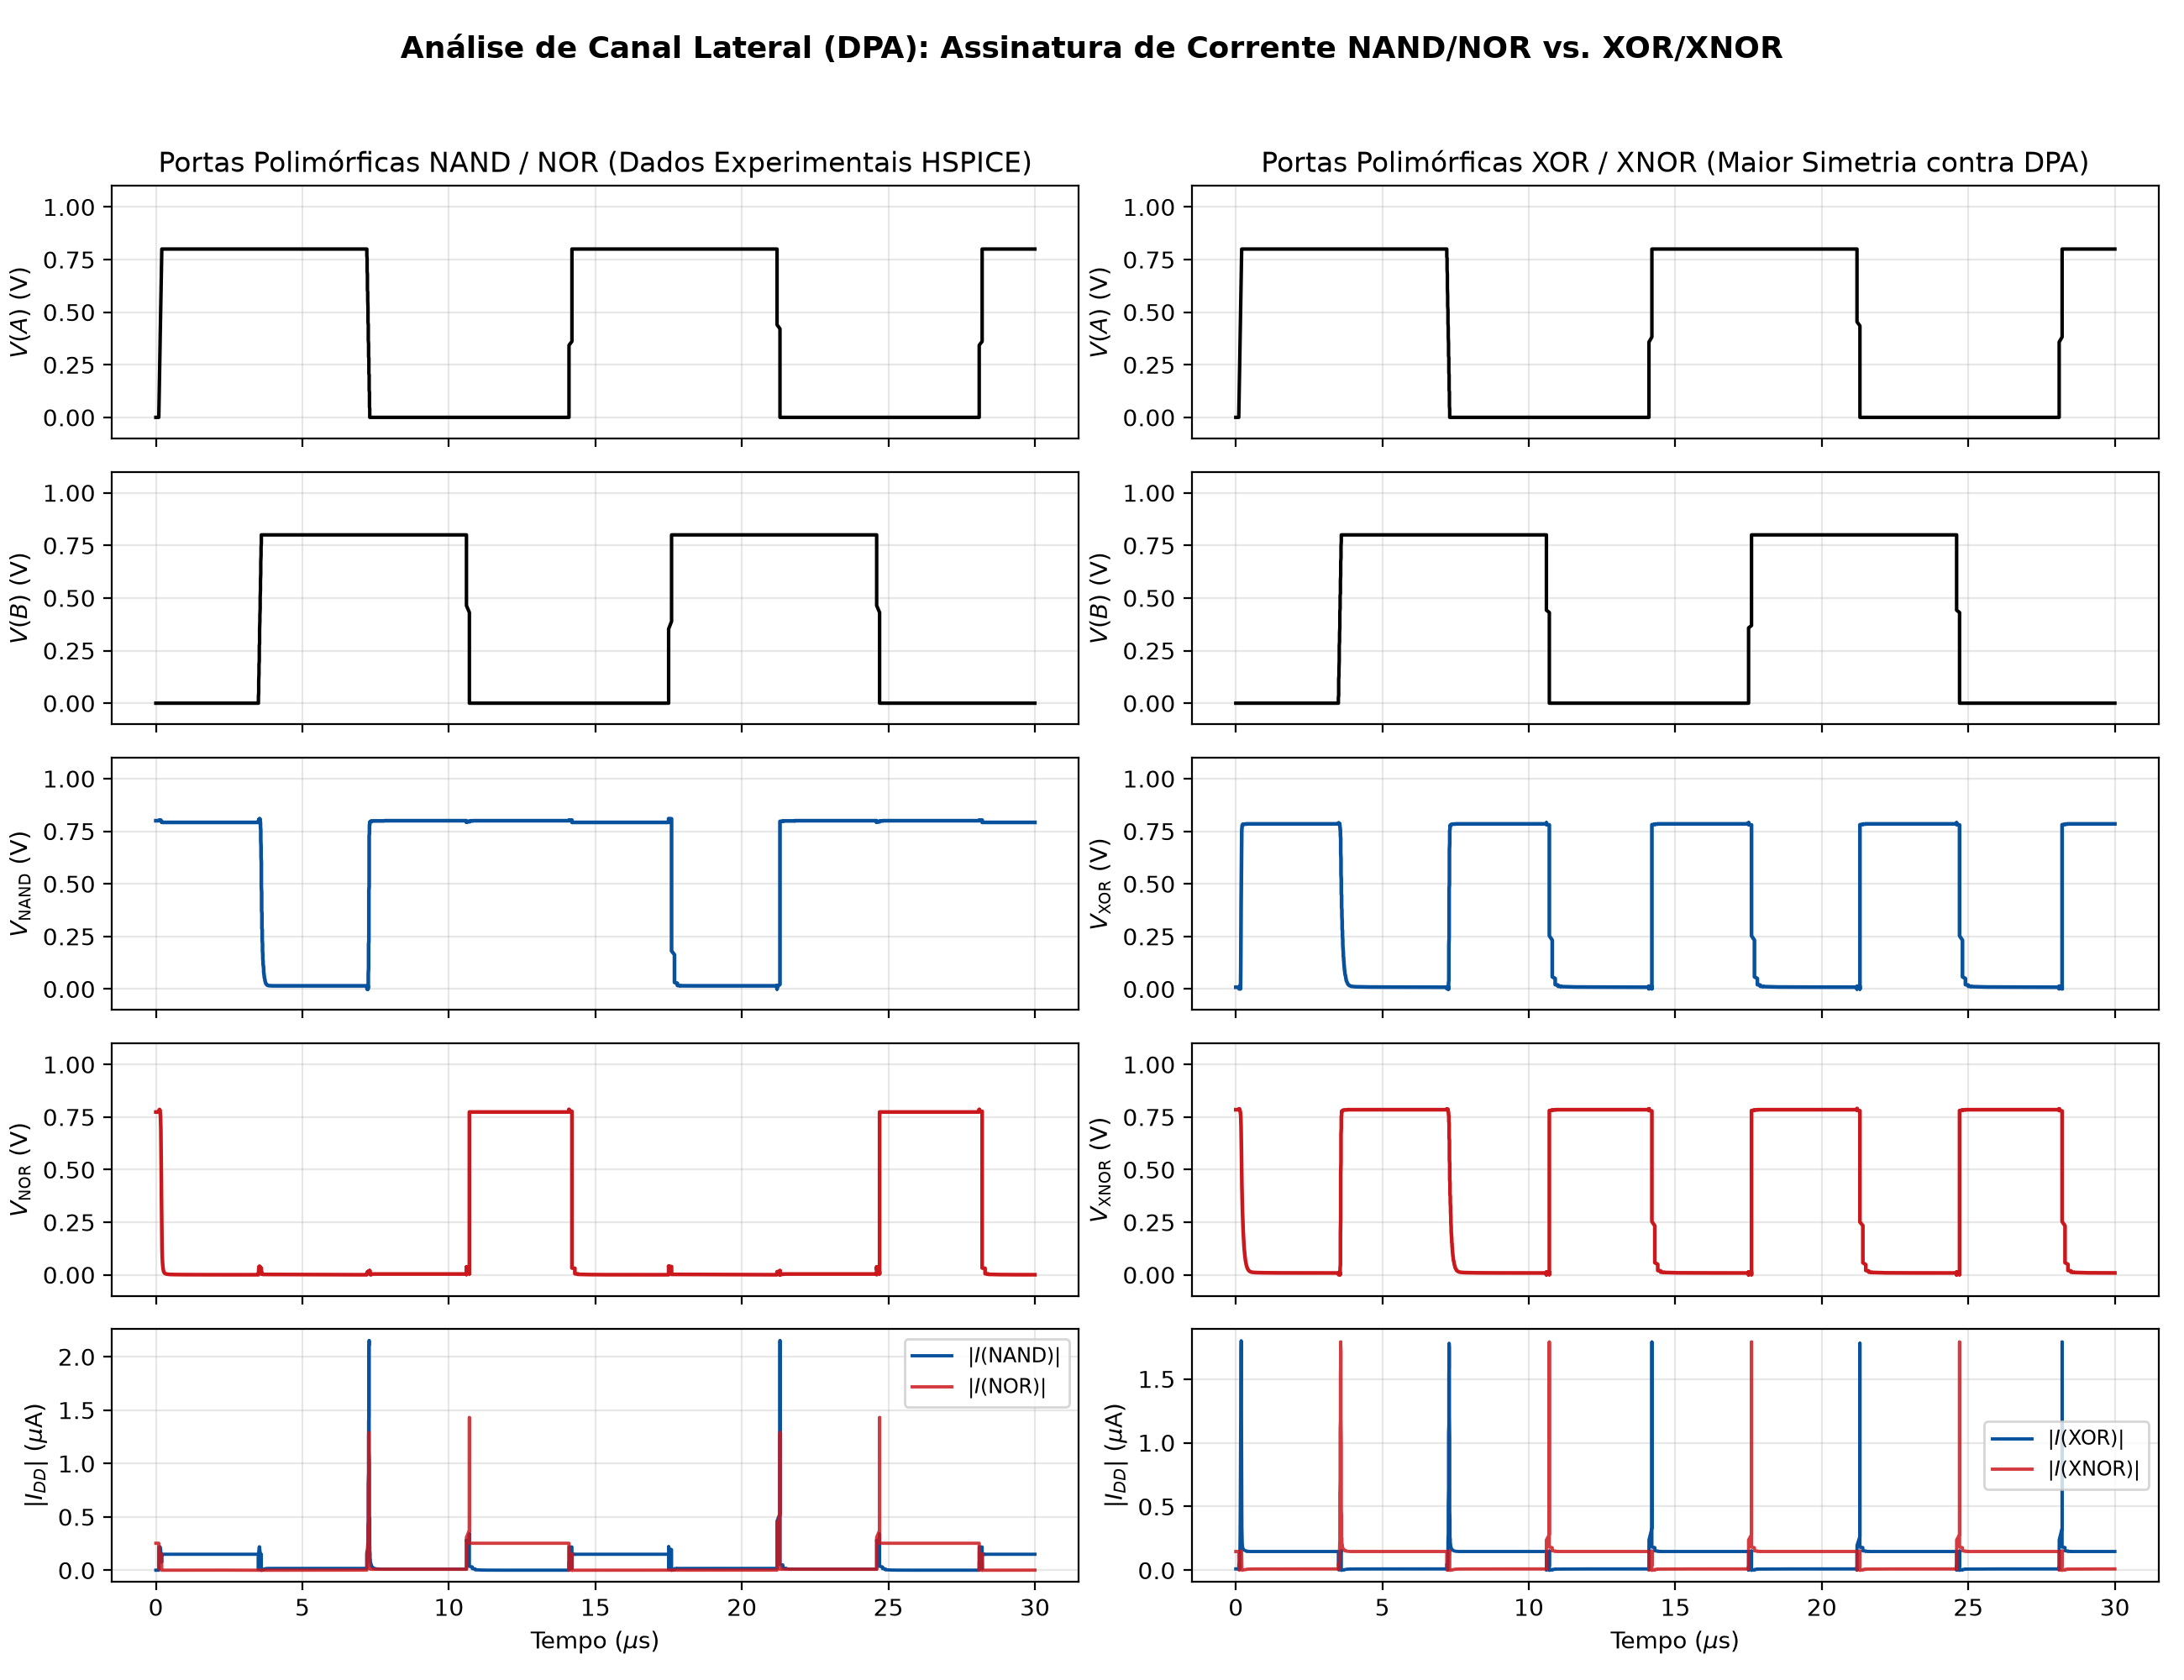
\includegraphics[width=0.92\textwidth]{m03_dpa_assinatura_corrente.png}
\caption{Side-channel DPA current signature comparison ($|I_{DD}|$) between \texttt{NAND}/\texttt{NOR} (left) and \texttt{XOR}/\texttt{XNOR} (right).}
\label{fig:m03_dpa}
\end{figure}

Across all 250 Monte Carlo samples (Figure~\ref{fig:m03_mc3d}), even under severe supply rail fluctuations ($V_{DD} \in [0.47,\ 1.15]\ \text{V}$), all four gates maintained $100.0\%$ logic accuracy with clean separation between \texttt{'0'} and \texttt{'1'} around $0.40\ \text{V}$. Cross-validation on the $5 \times 5$ \texttt{ngspice-47} grid (\texttt{ngspice\_supply\_sweep.csv}, Figure~\ref{fig:m03_hist_ret}) confirmed static margins $(V_{00} - V_{11})$ between $0.531\ \text{V}$ and $1.012\ \text{V}$ whenever $V_{DD} \ge 0.725\ \text{V}$ or $V_{SS} \ge -0.05\ \text{V}$, narrowing to $0.153\ \text{V}$ only at the worst-case corner ($V_{DD}=0.65\ \text{V},\ V_{SS}=-0.10\ \text{V}$, where $V_{00}=0.060\ \text{V}$ and $V_{11}=-0.093\ \text{V}$). For floating-node retention (\texttt{bblc1}), following excitation pulses at $40$ and $80\ \mu\text{s}$, the node stabilized at distinct plateaus of $0.65\ \text{V}$ ($100\ \text{ns}$), $0.30\ \text{V}$ ($250\ \text{ns}$), and $0.20\ \text{V}$ ($500\ \text{ns}$) through $111\ \mu\text{s}$.

\begin{figure}[htbp]
\centering
\begin{subfigure}{\textwidth}
  \centering
  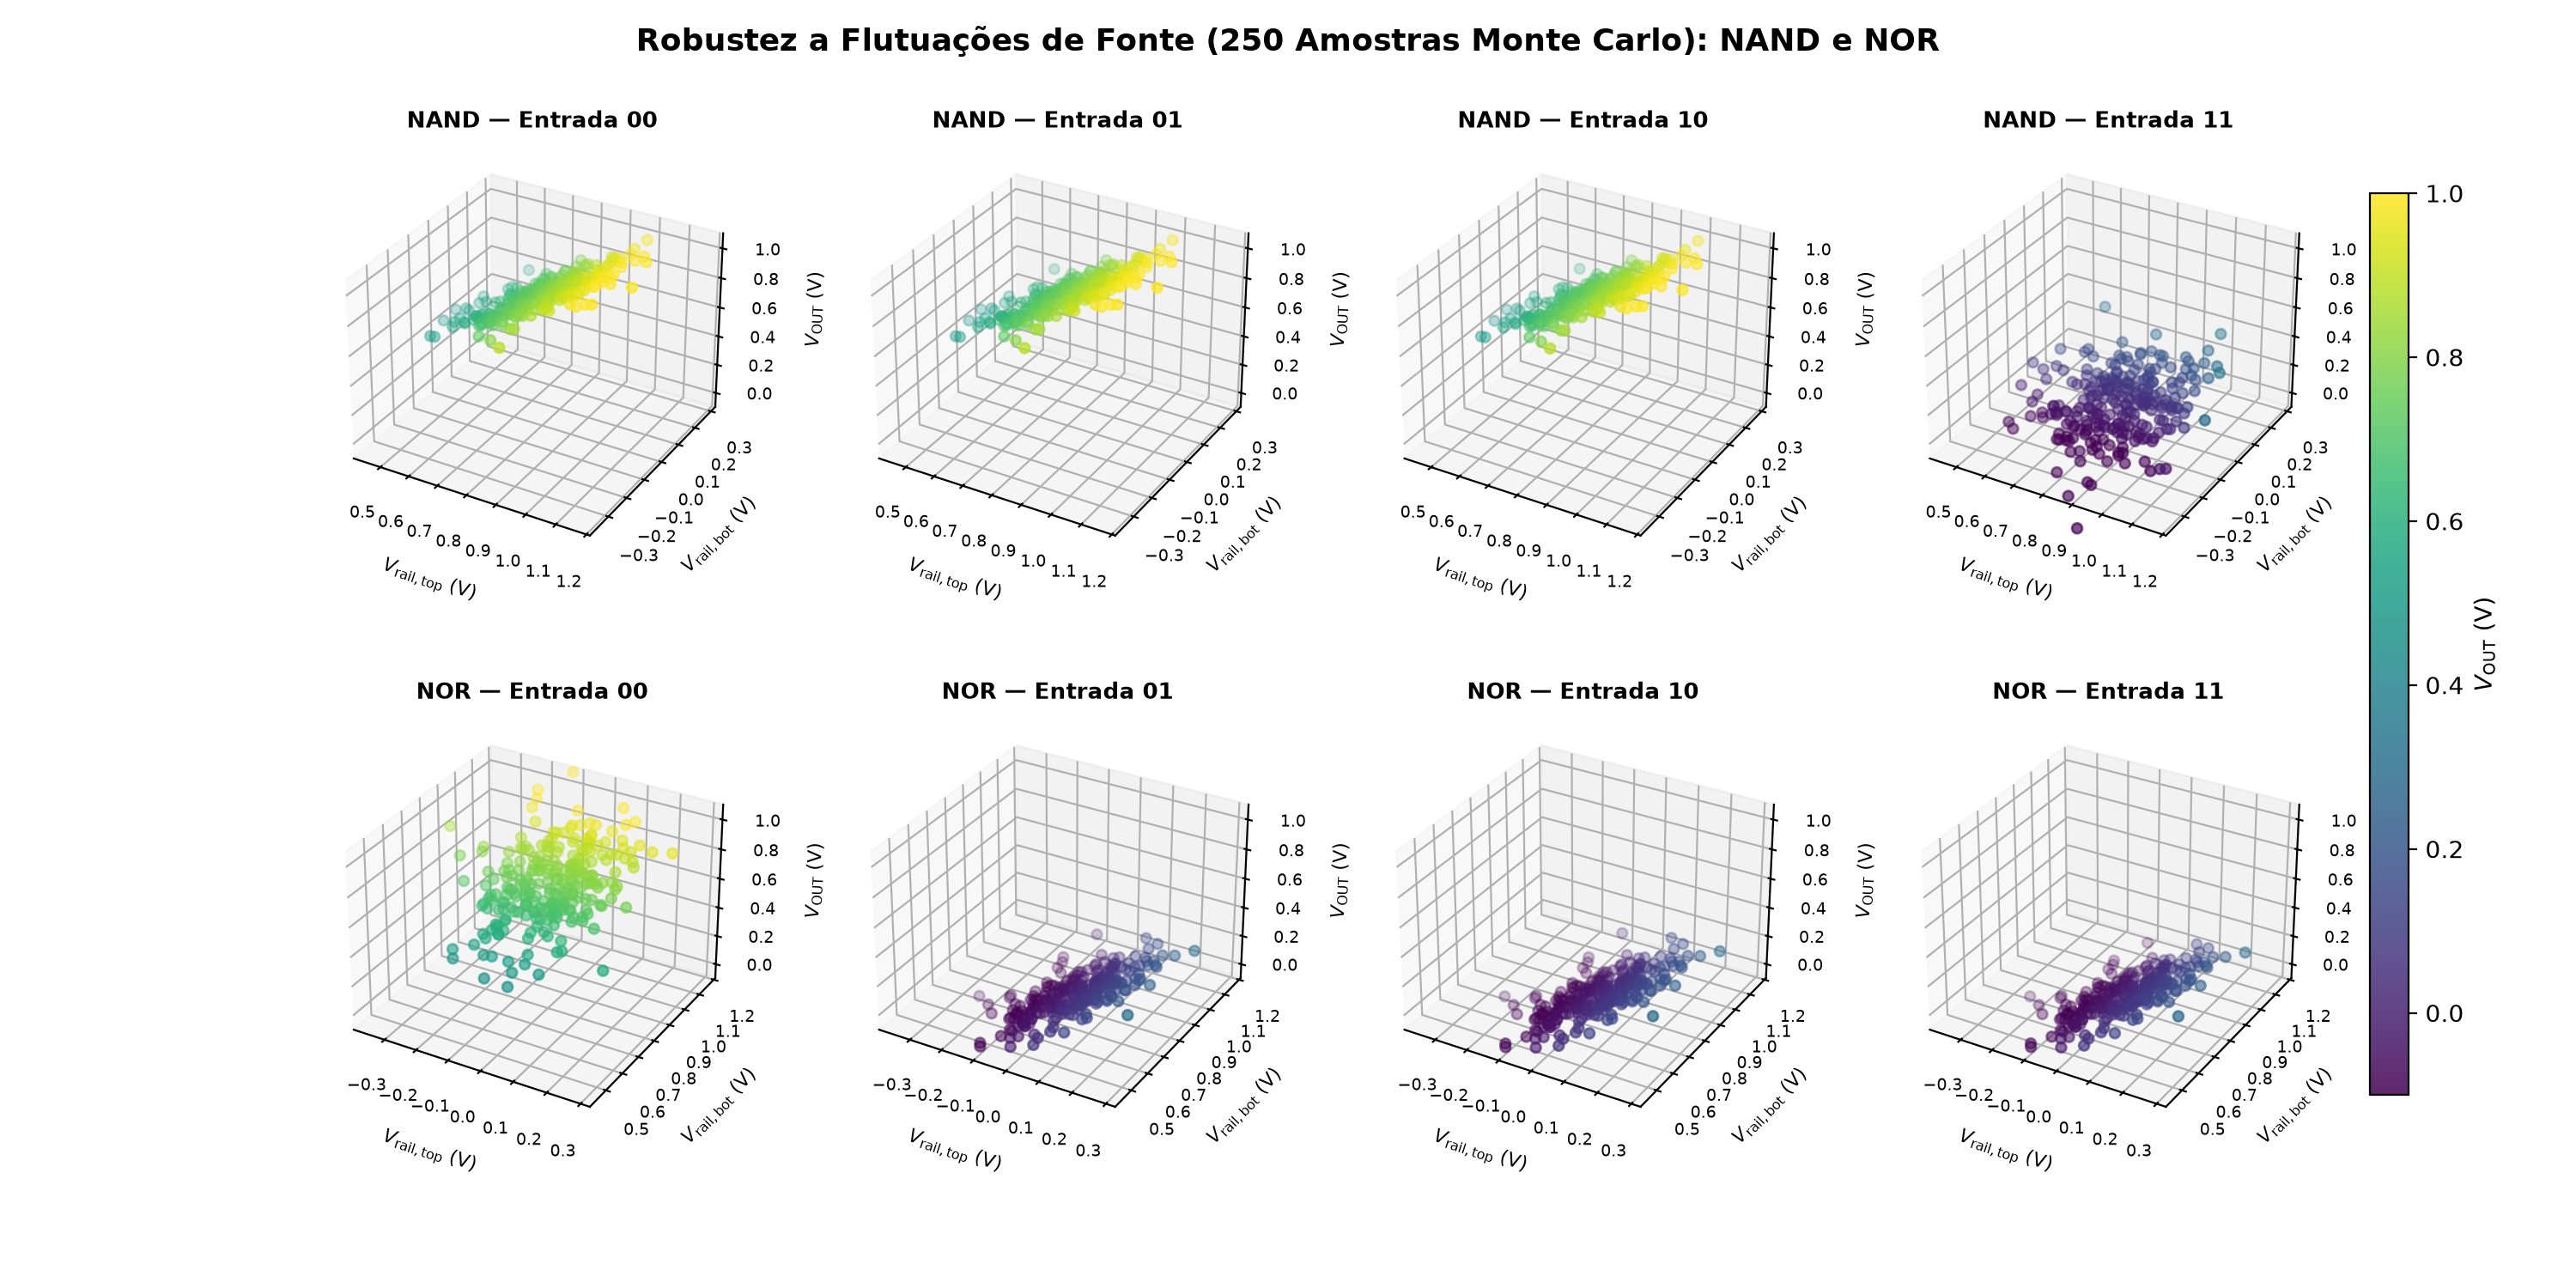
\includegraphics[width=0.95\textwidth]{m03_robustez_3d_nand_nor.png}
  \caption{\texttt{NAND} and \texttt{NOR} gates.}
  \label{fig:m03_3d_nn}
\end{subfigure}
\par\medskip
\begin{subfigure}{\textwidth}
  \centering
  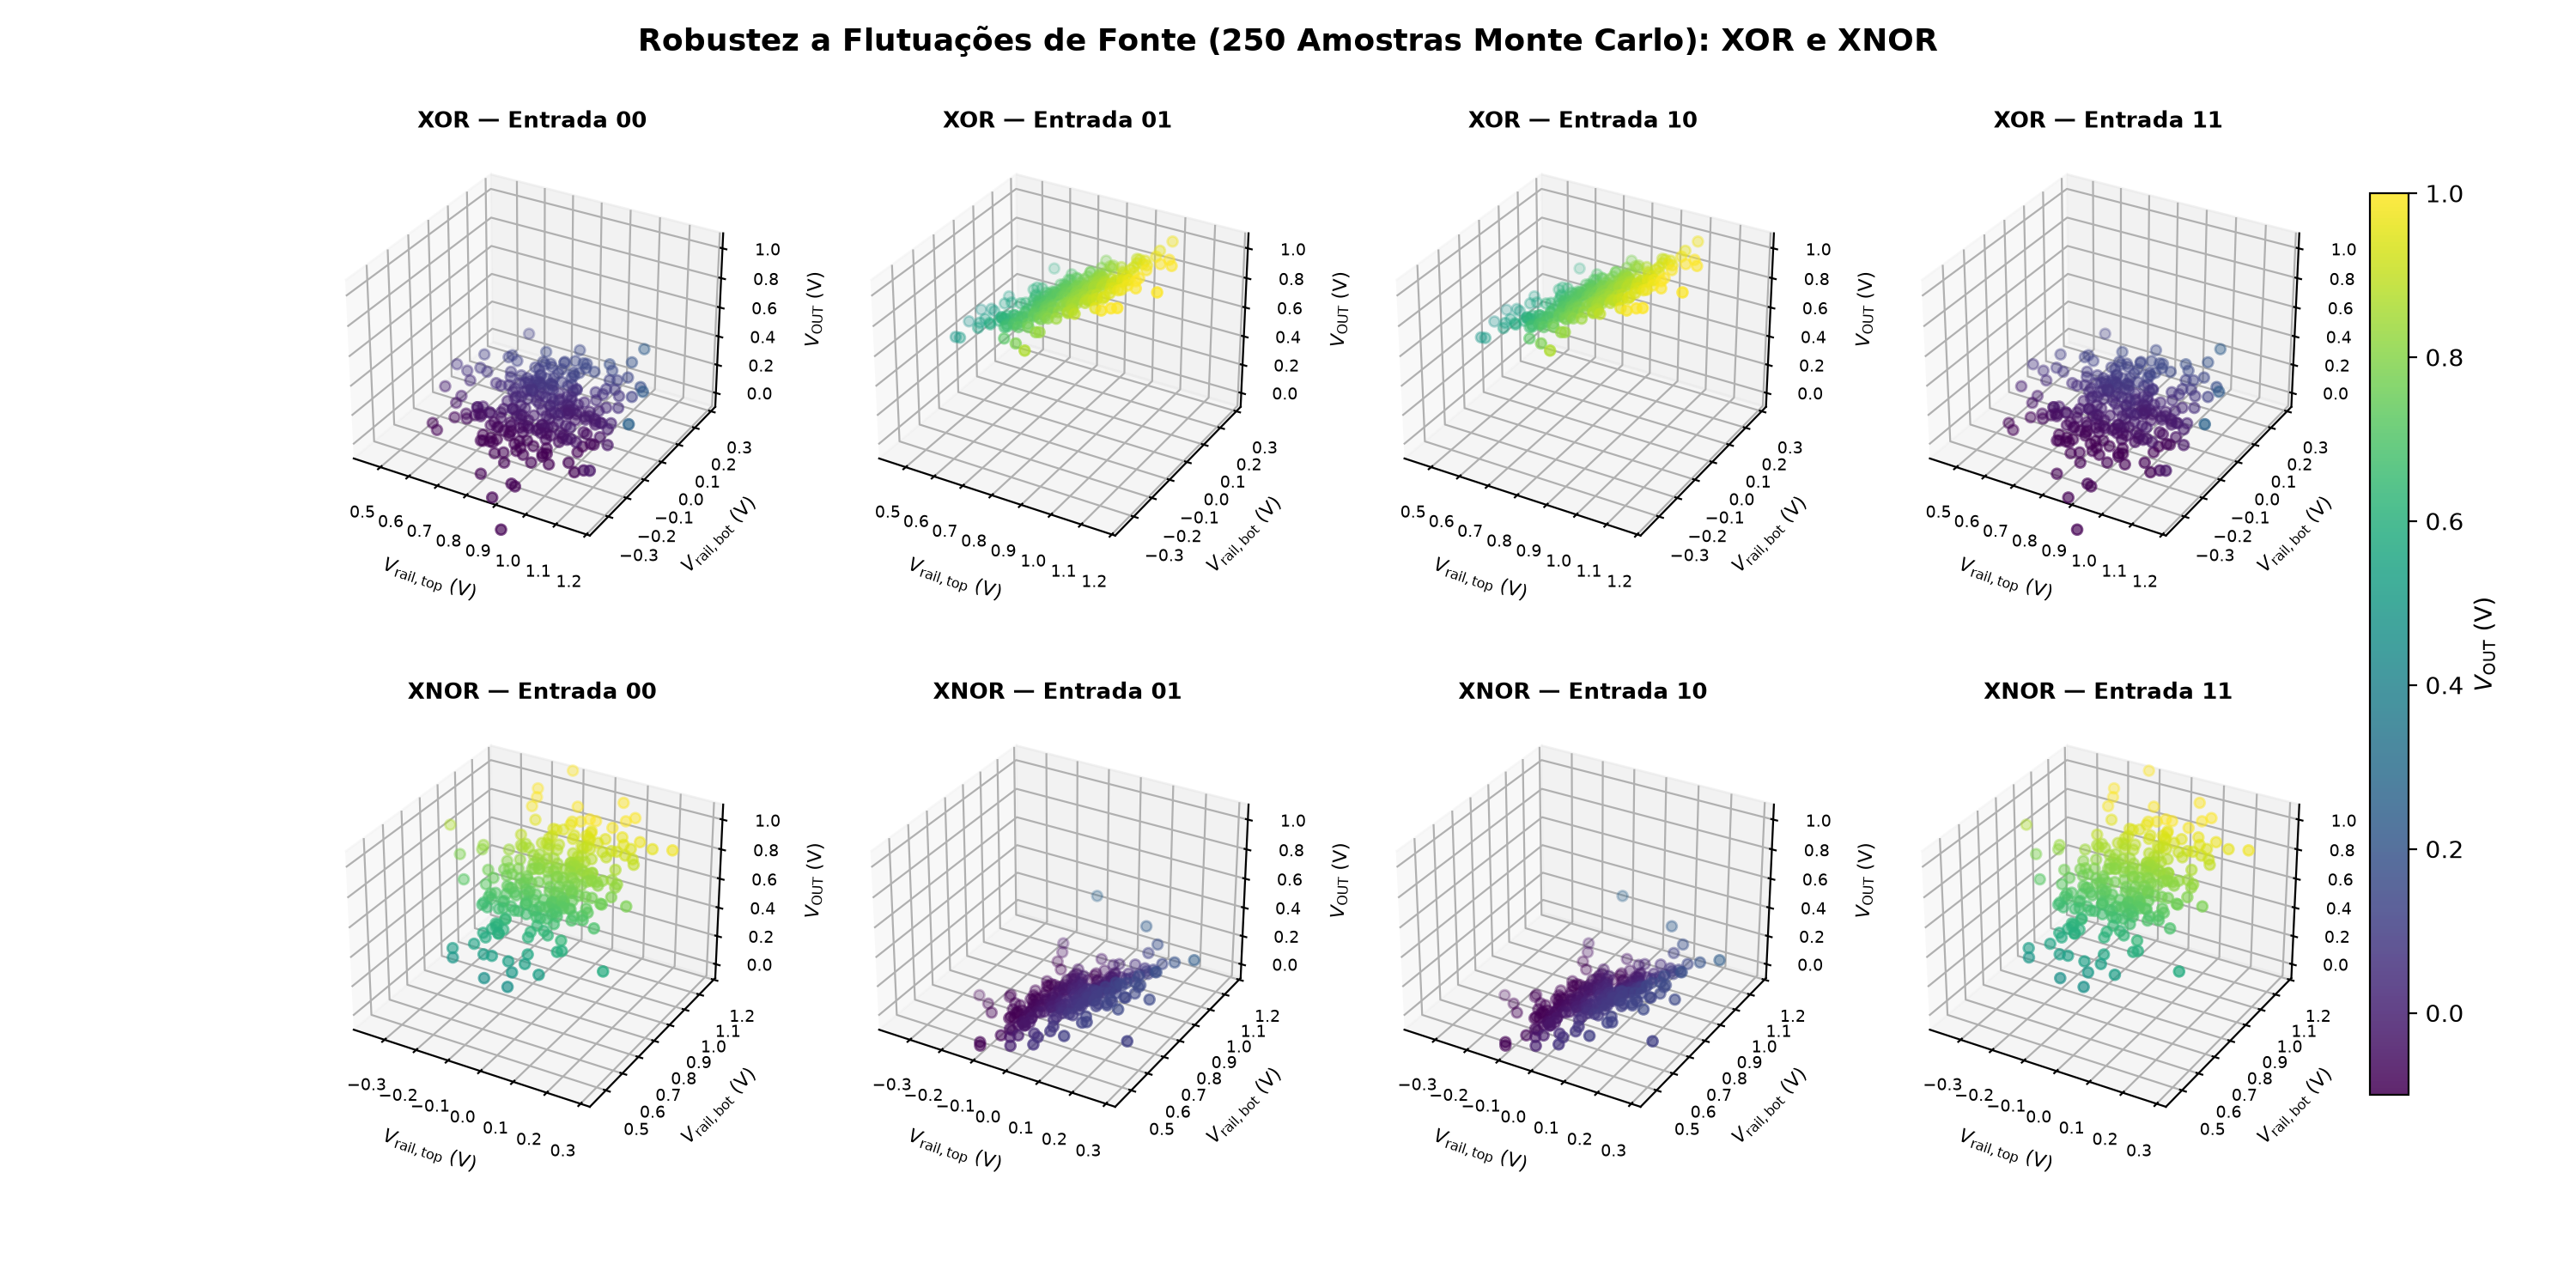
\includegraphics[width=0.95\textwidth]{m03_robustez_3d_xor_xnor.png}
  \caption{\texttt{XOR} and \texttt{XNOR} gates.}
  \label{fig:m03_3d_xx}
\end{subfigure}
\caption{3D robustness surfaces ($V_{\mathrm{rail,top}} \times V_{\mathrm{rail,bot}} \times V_{\mathrm{OUT}}$) across 250 Monte Carlo samples per input vector.}
\label{fig:m03_mc3d}
\end{figure}

\begin{figure}[htbp]
\centering
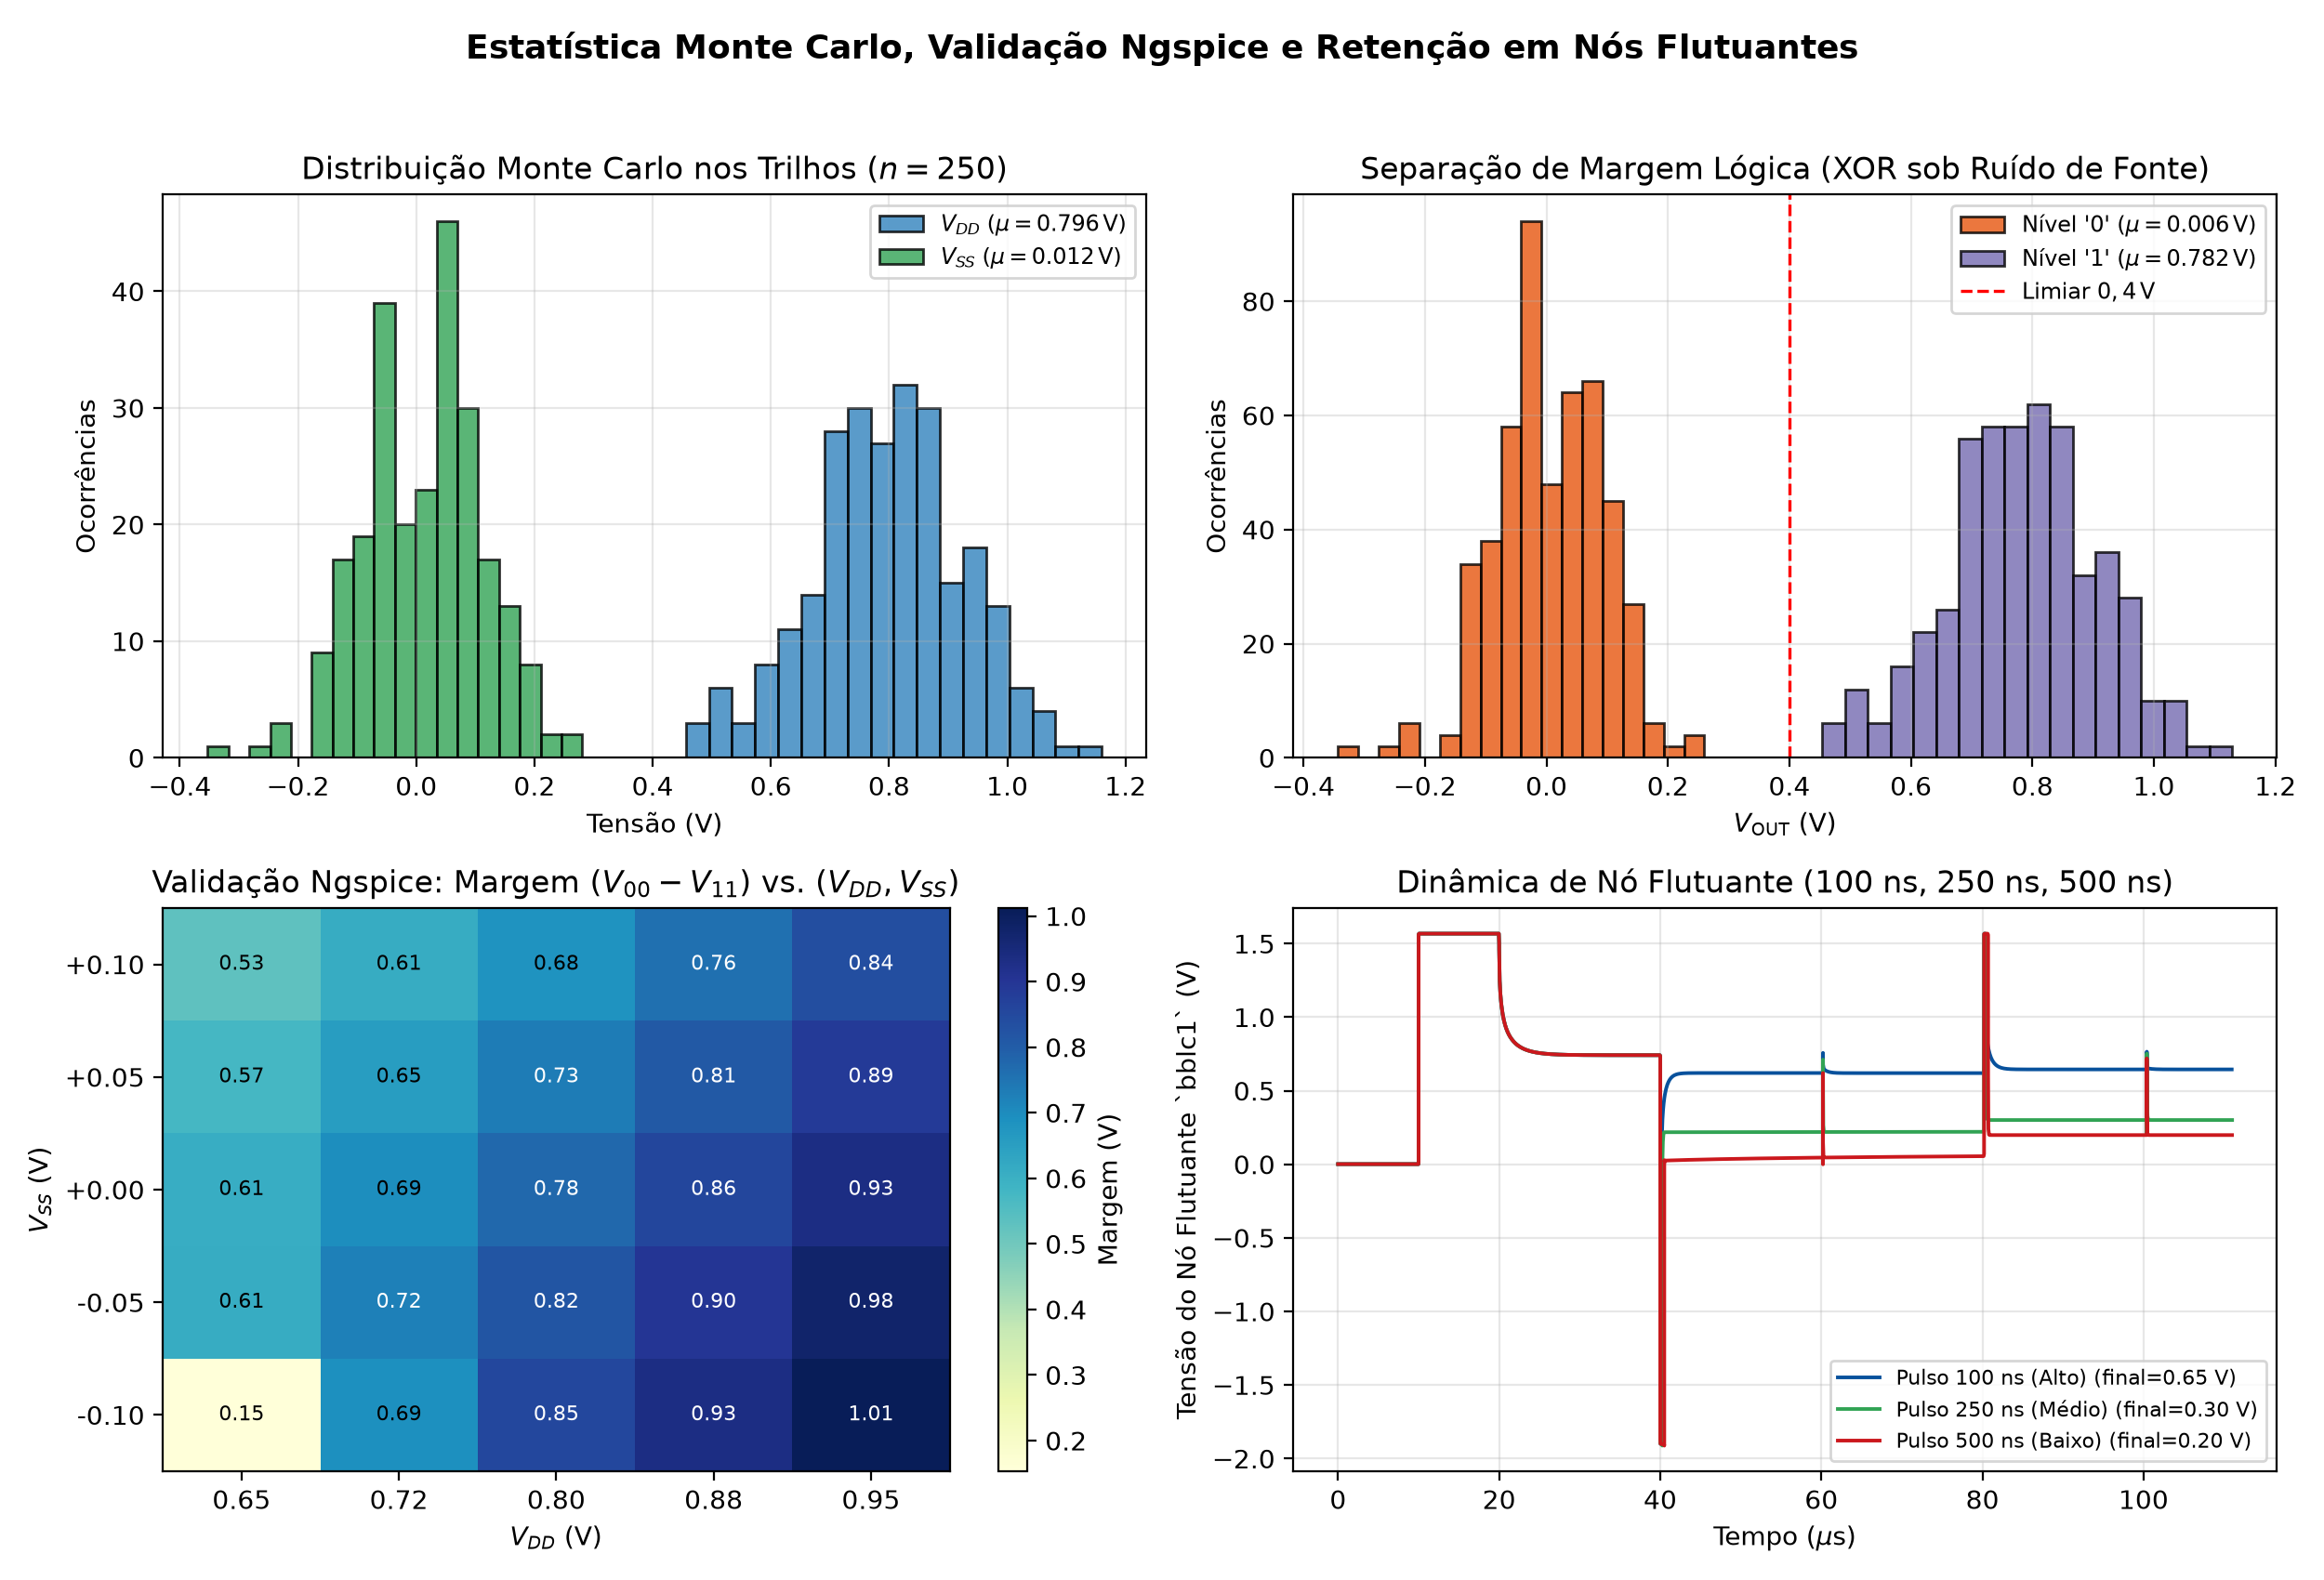
\includegraphics[width=0.92\textwidth]{m03_histogramas_e_retencao.png}
\caption{Monte Carlo rail distribution (top left), \texttt{XOR} logic-level separation (top right), \texttt{ngspice-47} $V_{DD}\times V_{SS}$ margin map (bottom left), and floating-node \texttt{bblc1} retention up to $111\ \mu\text{s}$ (bottom right).}
\label{fig:m03_hist_ret}
\end{figure}

\subsection{6T SRAM Cell with Retention Locking (Mechanism B)}\label{sec:res_sram}

The 6T SRAM cell passed all eleven transient and static acceptance criteria for Mechanism B, as summarized in Table~\ref{tab:sram_results}. During the $30\ \text{ns}$ transient simulation (Figure~\ref{fig:m04_tran}), under $\text{Key} = 0$, the bit \texttt{'1'} written in $0\text{--}6\ \text{ns}$ is stably retained after wordline de-assertion with $V(q) = 0.9768\ \text{V}$ and $V(qb) = 0.0020\ \text{V}$ at $t=12\ \text{ns}$ ($\Delta V_{\mathrm{Key0}} = 0.9747\ \text{V} > 0.80\ \text{V}$). Once $\text{Key}$ switches to $1$ ($t = 15\ \text{ns}$), while keeping $V_{DD} = 1.0\ \text{V}$ and $V_{SS} = 0.0\ \text{V}$ constant, simultaneous inversion of pull-up (\textit{p-FET} $\to$ \textit{n-FET}) and pull-down (\textit{n-FET} $\to$ \textit{p-FET}) devices triggers immediate collapse of the stored bit ($\Delta V_{\mathrm{Collapse1}} = 0.0841\ \text{V} < 0.15\ \text{V}$ at $18\ \text{ns}$). In Phase~4 ($20\text{--}30\ \text{ns}$), even after forcing the opposite bit while $\mathrm{WL}$ is asserted, the cell collapses again as soon as $\mathrm{WL}$ closes ($\Delta V_{\mathrm{Key1}} = 0.0762\ \text{V}$ at $28\ \text{ns}$).

\begin{table}[htbp]
\centering
\caption{Transient ($30\ \text{ns}$) and static noise margin (SNM) metrics of the 6T SRAM cell (\texttt{metricas\_sram\_6t.csv}).}
\label{tab:sram_results}
\footnotesize
\begin{tabular}{l c c c}
\toprule
\textbf{Extracted Metric} & \textbf{Simulated Value} & \textbf{Acceptance Criterion} & \textbf{Status} \\
\midrule
$V(q)_{\mathrm{Hold}}$ ($\text{Key}=0,\ t=12\ \text{ns}$)   & $0.9768\ \text{V}$ & $> 0.80\ \text{V}$ & Passed \\
$V(qb)_{\mathrm{Hold}}$ ($\text{Key}=0,\ t=12\ \text{ns}$)  & $0.0020\ \text{V}$ & $< 0.20\ \text{V}$ & Passed \\
$\Delta V_{\mathrm{Key0}}$ ($t=12\ \text{ns}$)              & $0.9747\ \text{V}$ & $> 0.80\ \text{V}$ & Passed \\
$\Delta V_{\mathrm{Collapse1}}$ ($t=18\ \text{ns}$)         & $0.0841\ \text{V}$ & $< 0.15\ \text{V}$ & Passed \\
$\Delta V_{\mathrm{Key1}}$ ($t=28\ \text{ns}$)              & $0.0762\ \text{V}$ & $< 0.15\ \text{V}$ & Passed \\
$\mathrm{SNM}_{\mathrm{Hold}}$ ($\text{Key}=0,\ \mathrm{WL}=0\ \text{V}$)           & $167.12\ \text{mV}$ & $> 150\ \text{mV}$ & Passed \\
$\mathrm{SNM}_{\mathrm{Read,Unassisted}}$ ($\text{Key}=0,\ \mathrm{WL}=1.0\ \text{V}$) & $0.00\ \text{mV}$ & $0\ \text{mV}$ (\textit{Read Disturb}) & Diagnosed \\
$\mathrm{SNM}_{\mathrm{Read,Assist}}$ ($\text{Key}=0,\ \mathrm{WL}=0.30\ \text{V}$) & $66.23\ \text{mV}$ & $> 50\ \text{mV}$ & Passed \\
$\mathrm{SNM}_{\mathrm{Hold}}$ ($\text{Key}=1,\ \mathrm{WL}=0\ \text{V}$)           & $0.00\ \text{mV}$ & $= 0\ \text{mV}$ & Passed \\
$\mathrm{SNM}_{\mathrm{Read,Assist}}$ ($\text{Key}=1,\ \mathrm{WL}=0.30\ \text{V}$) & $0.00\ \text{mV}$ & $= 0\ \text{mV}$ & Passed \\
$\mathrm{SNM}_{\mathrm{Read,Unassisted}}$ ($\text{Key}=1,\ \mathrm{WL}=1.0\ \text{V}$) & $0.00\ \text{mV}$ & $= 0\ \text{mV}$ & Passed \\
\bottomrule
\end{tabular}
\end{table}

\begin{figure}[htbp]
\centering
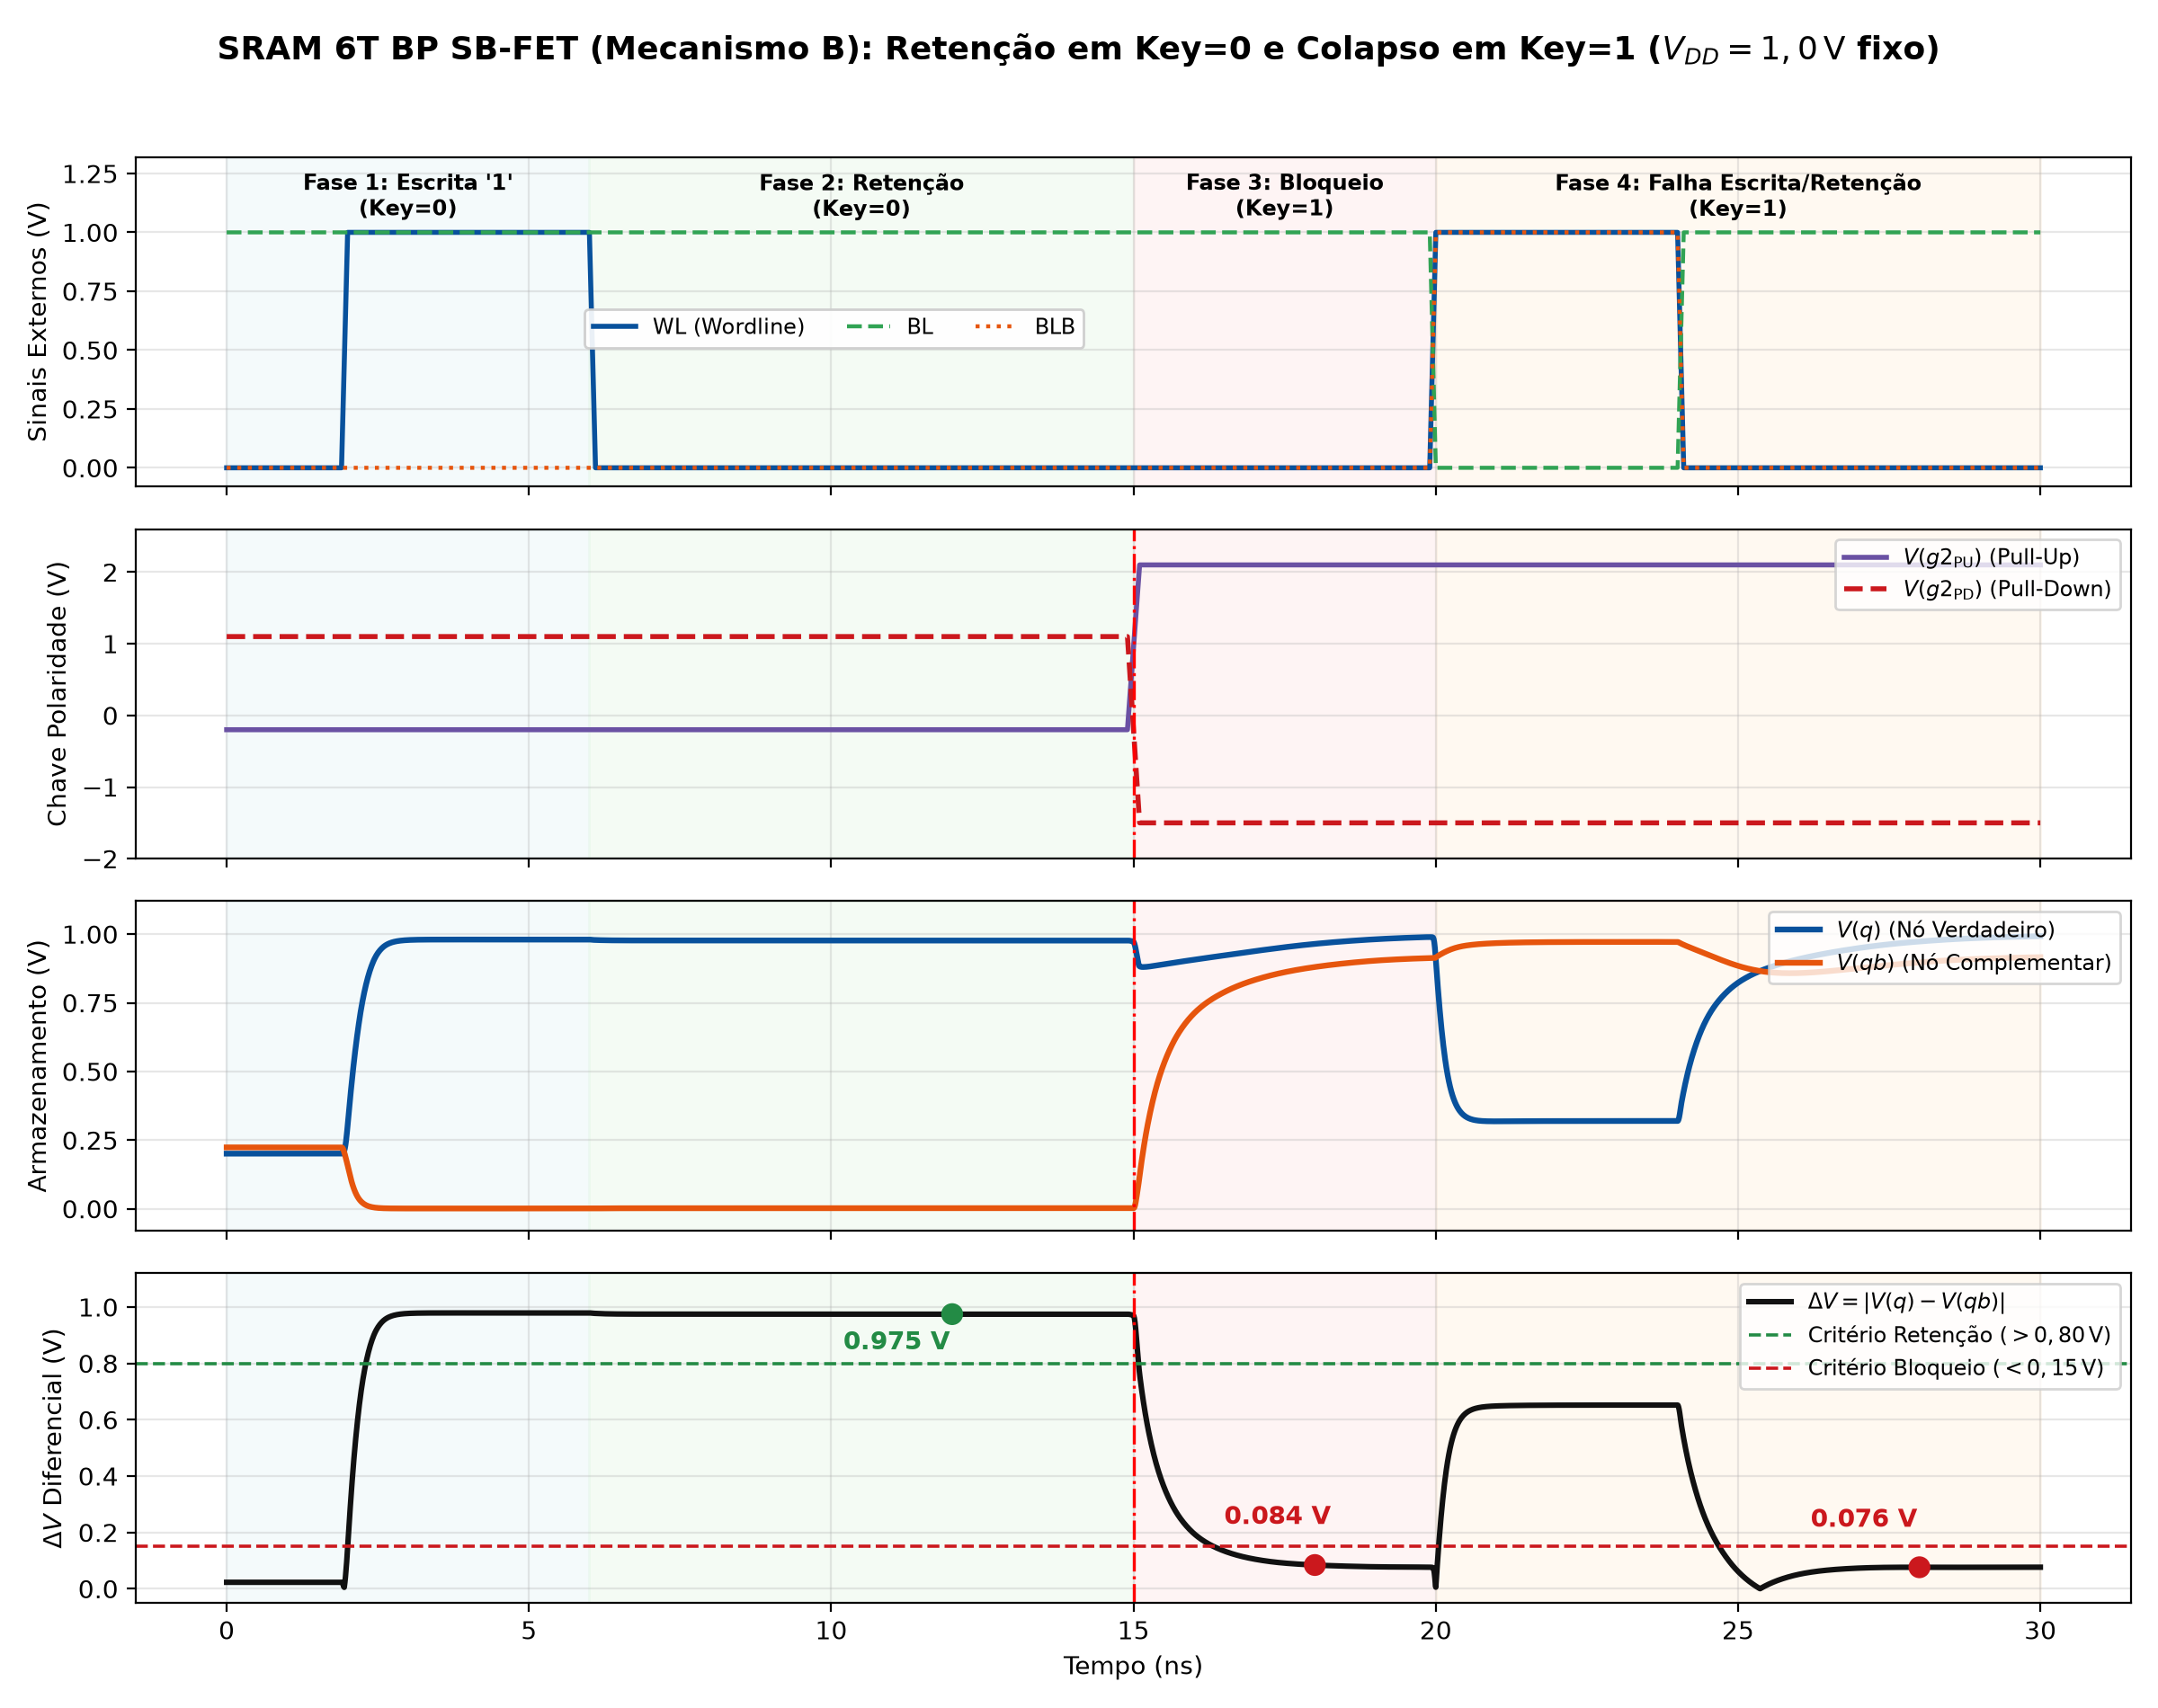
\includegraphics[width=0.92\textwidth]{m04_sram_transiente_30ns.png}
\caption{Four-phase $30\ \text{ns}$ transient simulation of the 6T SRAM cell: write and stable retention under $\text{Key}=0$ ($0\text{--}15\ \text{ns}$) followed by self-destruction and rewrite failure under $\text{Key}=1$ ($15\text{--}30\ \text{ns}$).}
\label{fig:m04_tran}
\end{figure}

\begin{figure}[htbp]
\centering
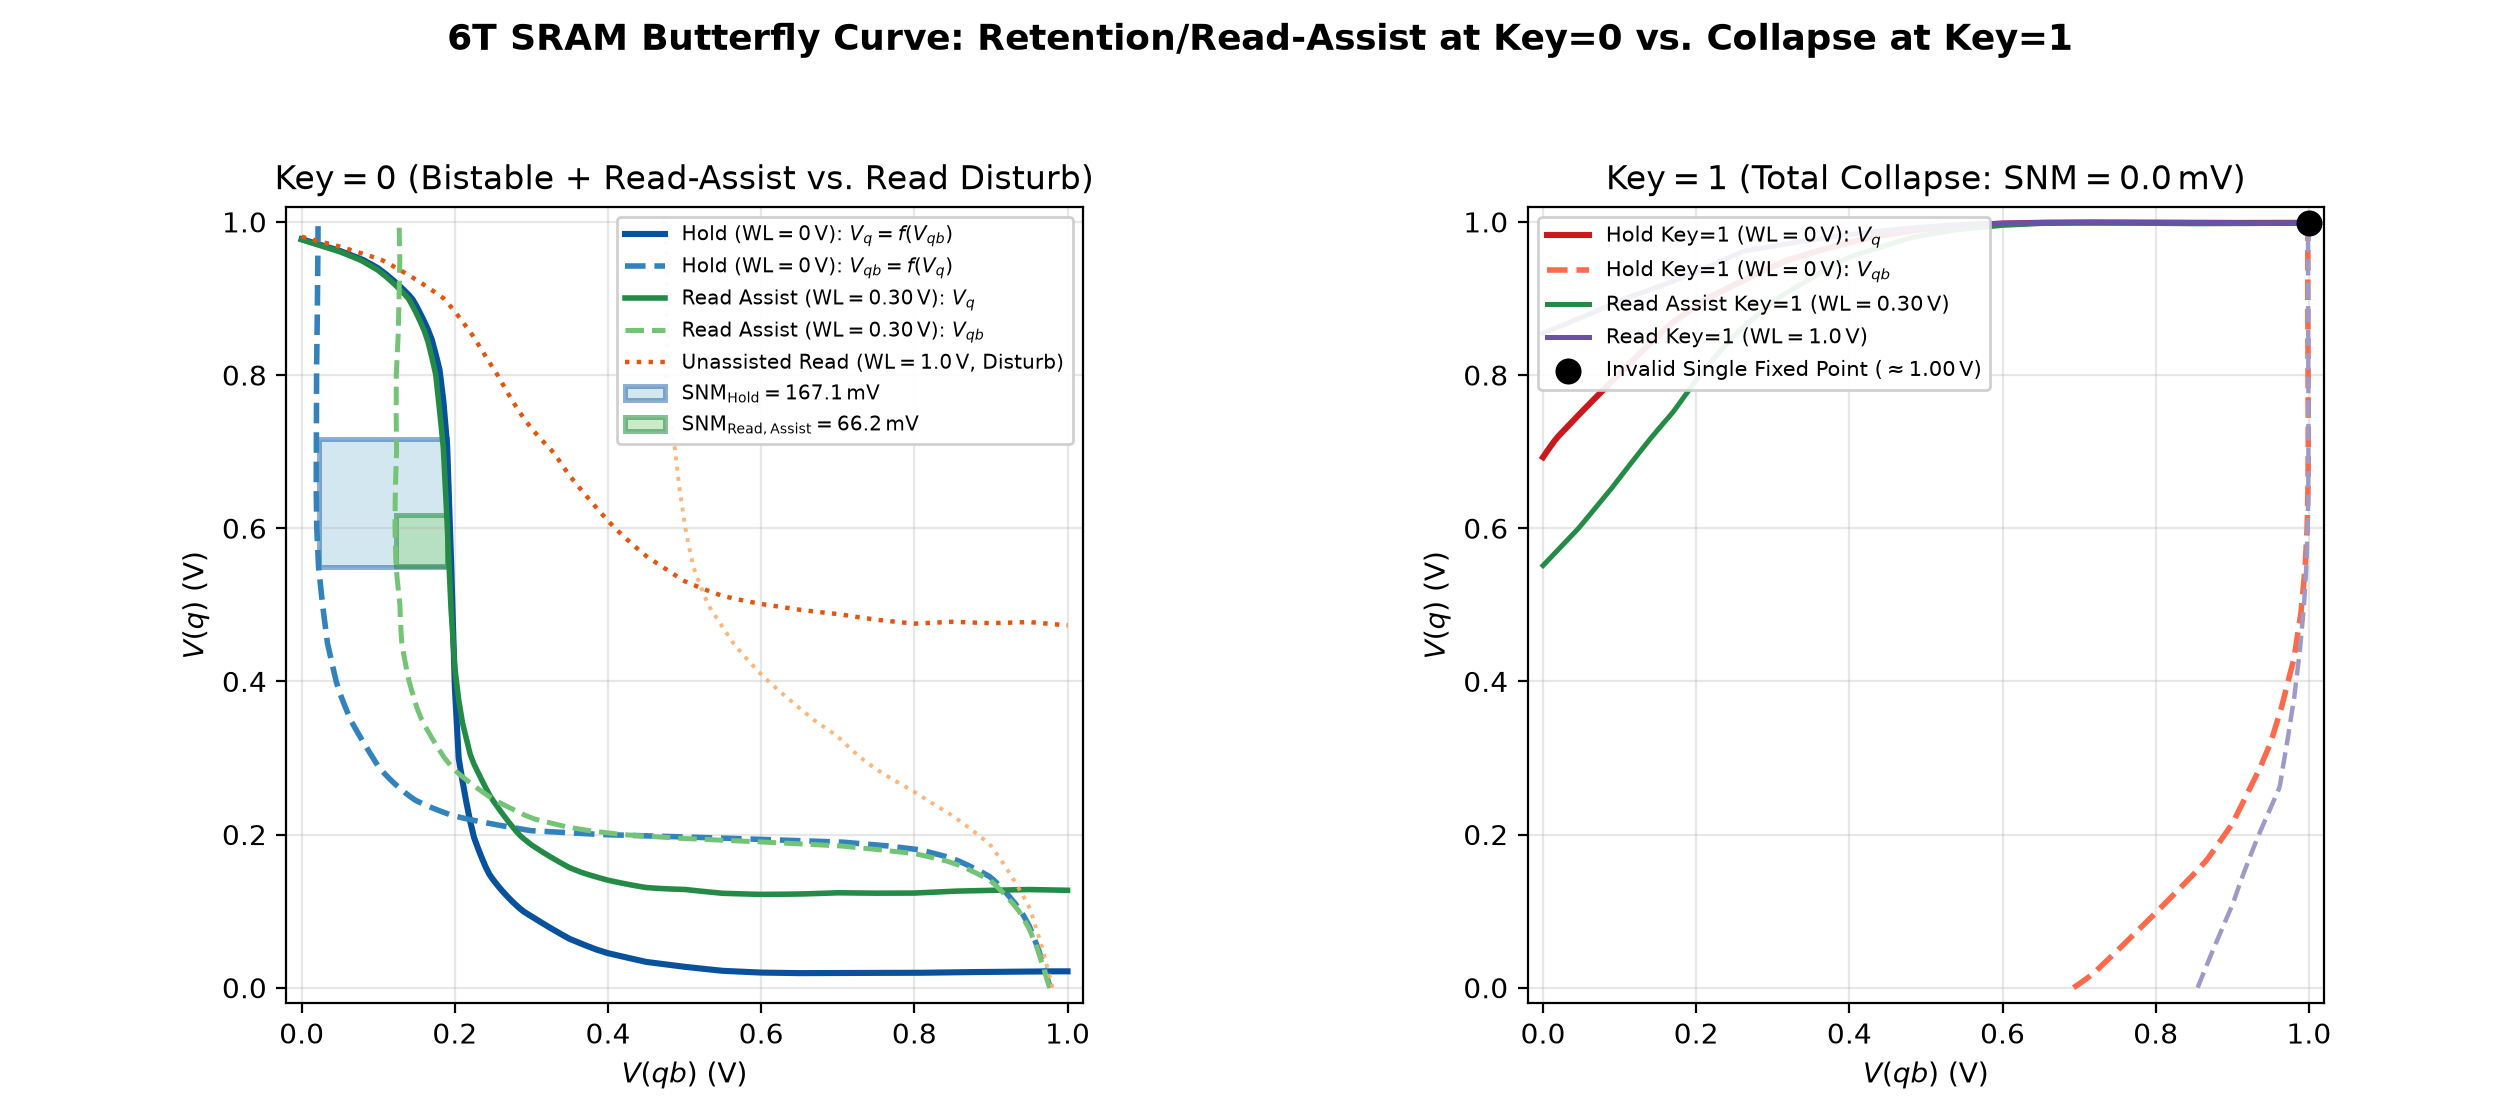
\includegraphics[width=0.92\textwidth]{m04_sram_curva_borboleta_snm.png}
\caption{6T SRAM butterfly curves and maximum inscribed SNM squares for $\text{Key}=0$ (Hold, Read-Assist, and Unassisted Read showing \textit{Read Disturb}) and $\text{Key}=1$ (total monostable collapse).}
\label{fig:m04_snm}
\end{figure}

Two important physical findings emerged from the butterfly-curve analysis (Figure~\ref{fig:m04_snm}). First, simulations with the 4D \texttt{v2} model revealed that the initially proposed $V_{g2,\mathrm{PU}} = -0.5\ \text{V}$ ($V_{g2,s} = -1.5\ \text{V}$) bias reduces \textit{p-FET} current from $1.79$ to $0.37\ \mu\text{A}$ (at $V_{gp}=-1.0\ \text{V}$) due to flat-band shift, lowering $\mathrm{SNM}_{\mathrm{Hold}}$ to $49.4\ \text{mV}$; tuning to $V_{g2,\mathrm{PU}} = -0.2\ \text{V}$ ($V_{g2,s} = -1.2\ \text{V}$) fully restored symmetry without altering device widths $W$, recovering $\mathrm{SNM}_{\mathrm{Hold}} = 167.12\ \text{mV}$. Second, unassisted reading ($\mathrm{WL}=1.0\ \text{V}$) exhibited destructive \textit{Read Disturb} ($\mathrm{SNM}=0.00\ \text{mV}$), which was mitigated via \textit{Wordline Underdrive Read-Assist} at $\mathrm{WL}=0.30\ \text{V}$, restoring $\mathrm{SNM}_{\mathrm{Read,Assist}} = 66.23\ \text{mV}$ while all $\text{Key}=1$ conditions remained locked at $\mathrm{SNM}=0.00\ \text{mV}$.

\subsection{Cryptographic Polymorphic Full Adder (28 Transistors)}\label{sec:res_fa}

In the 28-transistor polymorphic Full Adder (Module~\texttt{05}), the authorized key $K_1 K_0 = 00$ achieved $100.00\%$ truth-table accuracy across all eight minterms ($000 \to 111$, Figure~\ref{fig:m05_wave}), maintaining over $94\%$ swing on \texttt{Sum} ($1.5\ \text{V}$ domain: \texttt{'0'} $\le 0.0012\ \text{V}$, \texttt{'1'} $\ge 1.4129\ \text{V}$) and over $92\%$ swing on \texttt{Cout} ($0.8\ \text{V}$ domain: \texttt{'0'} $\le 0.0124\ \text{V}$, \texttt{'1'} $\ge 0.7526\ \text{V}$) across three cascaded logic levels.

\begin{table}[htbp]
\centering
\caption{Functional corruption and Hamming Distance (HD) per cryptographic key $(K_1, K_0)$ in the 28T Full Adder.}
\label{tab:fa_hamming}
\resizebox{\textwidth}{!}{%
\begin{tabular}{c l c c c c c c}
\toprule
\textbf{Key} $K_1K_0$ & \textbf{Configuration} (\texttt{XXOR1} + \texttt{Cout}) & \texttt{Sum} \textbf{Errors} & \textbf{HD} \texttt{Sum} & \texttt{Cout} \textbf{Errors} & \textbf{HD} \texttt{Cout} & \textbf{Total HD} (/16) & \textbf{Accuracy} \\
\midrule
\texttt{00} (Correct) & \texttt{XOR} + \texttt{NAND}  & $0/8$ & $0.0\%$   & $0/8$ & $0.0\%$  & $0\ (0.00\%)$   & $100.00\%$ \\
\texttt{01} (Wrong)   & \texttt{XNOR} + \texttt{NAND} & $8/8$ & $100.0\%$ & $3/8$ & $37.5\%$ & $11\ (68.75\%)$ & $31.25\%$  \\
\texttt{10} (Wrong)   & \texttt{XOR} + \texttt{NOR}   & $0/8$ & $0.0\%$   & $3/8$ & $37.5\%$ & $3\ (18.75\%)$  & $81.25\%$  \\
\texttt{11} (Wrong)   & \texttt{XNOR} + \texttt{NOR}  & $8/8$ & $100.0\%$ & $0/8$ & $0.0\%$  & $8\ (50.00\%)$  & $50.00\%$  \\
\bottomrule
\end{tabular}}
\end{table}

As shown in Table~\ref{tab:fa_hamming} and Figure~\ref{fig:m05_hd}, every incorrect key corrupts the arithmetic output without requiring extra dedicated locking transistors. At $K_1K_0 = 01$, inversion of $P \to \overline{P}$ propagates errors to both \texttt{Sum} ($100.0\%$) and \texttt{Cout} ($37.5\%$), yielding $\mathrm{HD}_{\mathrm{Total}} = 68.75\%$. At $K_1K_0 = 11$, De Morgan duality emerges: switching both \texttt{XXOR1} to \texttt{XNOR} ($\overline{P}$) and \texttt{XG1}--\texttt{XG3} to \texttt{NOR} produces $\overline{\overline{A+B} + \overline{\overline{P}+C_{\mathrm{in}}}} = (A+B)\cdot(\overline{P}+C_{\mathrm{in}}) = A\cdot B + C_{\mathrm{in}}\cdot(A\oplus B)$, restoring \texttt{Cout} while \texttt{Sum} remains $100.0\%$ inverted ($\mathrm{HD}_{\mathrm{Total}} = 50.00\%$).

\begin{figure}[htbp]
\centering
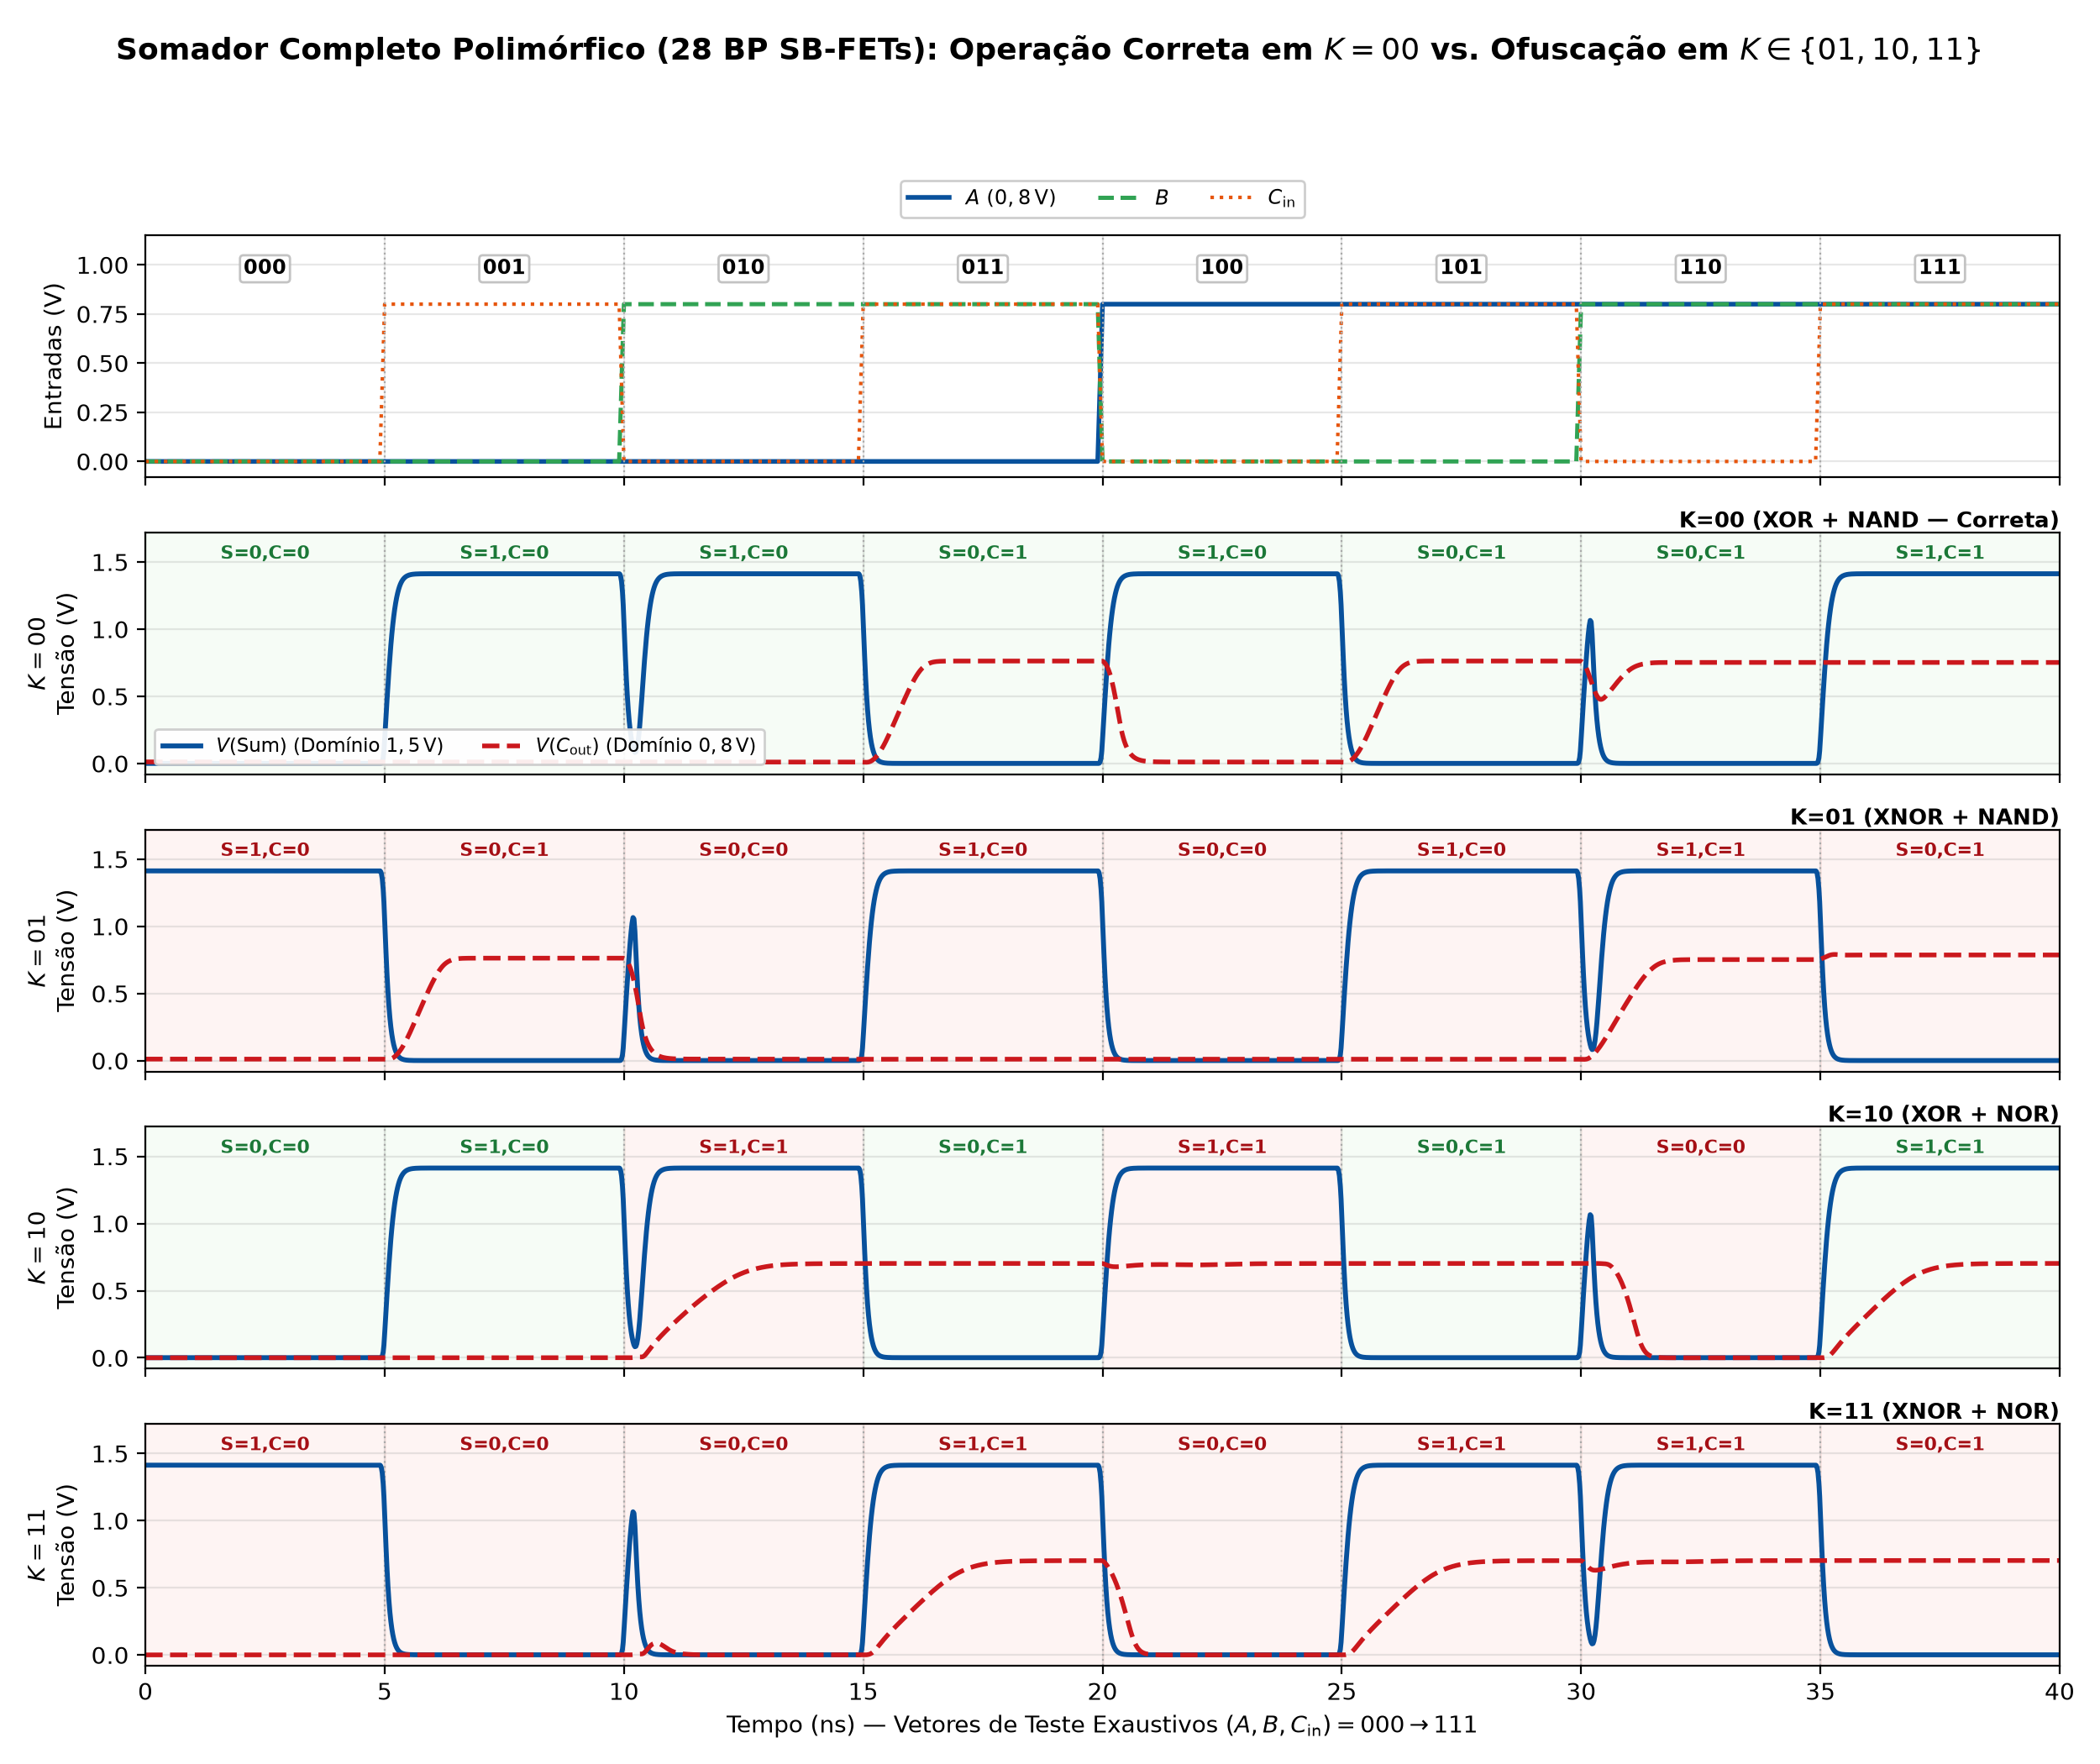
\includegraphics[width=0.92\textwidth]{m05_full_adder_waveforms.png}
\caption{Exhaustive transient waveforms ($40\ \text{ns}$, minterms \texttt{000} to \texttt{111}) of the 28-transistor polymorphic Full Adder across all four keys $K_1K_0$.}
\label{fig:m05_wave}
\end{figure}

\begin{figure}[htbp]
\centering
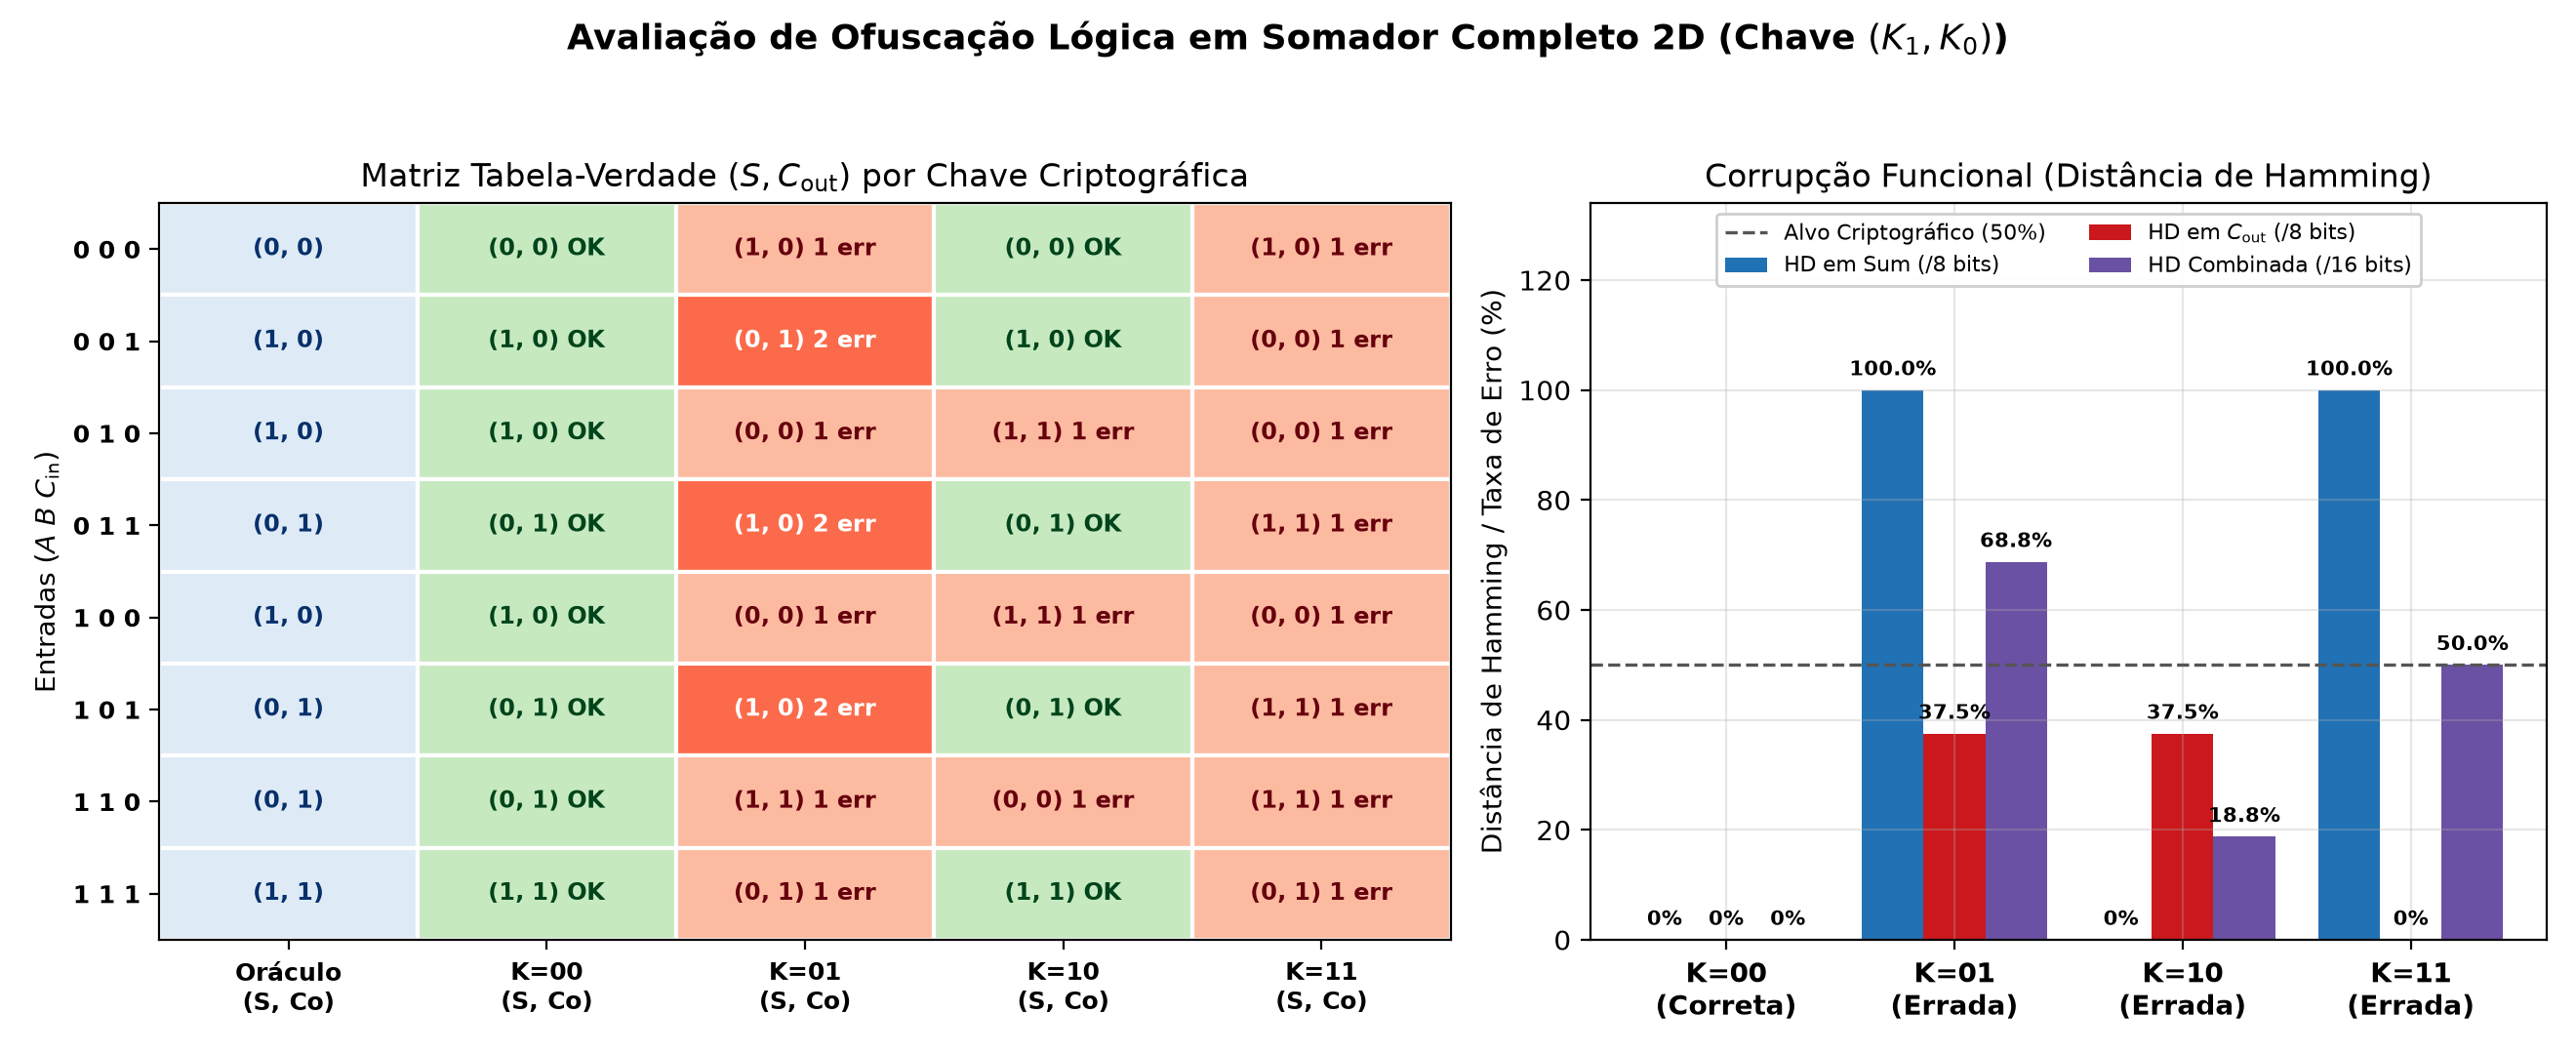
\includegraphics[width=0.92\textwidth]{m05_matriz_tabelas_verdade_hamming.png}
\caption{Truth-table matrix and Hamming Distance (HD) of the polymorphic Full Adder for keys \texttt{00}, \texttt{01}, \texttt{10}, and \texttt{11}.}
\label{fig:m05_hd}
\end{figure}

\subsection{Operating Boundaries under Non-Standard Voltages}\label{sec:res_boundary}

Sweeping 292 points inside the experimentally measured LUT domain (Module~\texttt{06}) confirmed that shifting supply, input, and polarity voltages can trigger all three hypothesized outcomes: preservation of the target function (\texttt{CORRETA}), transmutation into another digital Boolean function (\texttt{OUTRA\_FUNCAO}), or collapse into intermediate analog states (\texttt{INDEFINIDO\_ANALOGICO}), as summarized in Table~\ref{tab:boundary_summary}.

\begin{table}[htbp]
\centering
\caption{Classification of the 292 operating points simulated under non-standard voltages within the LUT domain.}
\label{tab:boundary_summary}
\resizebox{\textwidth}{!}{%
\begin{tabular}{l c c c c l}
\toprule
\textbf{Sub-experiment} & \textbf{Points} & \texttt{CORRETA} & \texttt{OUTRA\_FUNCAO} & \texttt{INDEFINIDO} & \textbf{Observed Equivalent Functions} \\
\midrule
\texttt{NAND}/\texttt{NOR} ($V_{DD}\times$ Pol.) & $70$  & $29$ & $35$ & $6$  & \texttt{NAND} ($13$), \texttt{NOR} ($17$), \texttt{CONST\_0} ($34$), \texttt{X} ($6$) \\
\texttt{NAND}/\texttt{NOR} ($V_{g2,n}\times V_{g2,p}$) & $72$  & $60$ & $0$  & $12$ & \texttt{NAND} ($27$), \texttt{NOR} ($33$), \texttt{X} ($12$) \\
\texttt{XOR}/\texttt{XNOR} ($V_{DD}\times V_{\mathrm{in}}$) & $100$ & $44$ & $46$ & $10$ & \texttt{XOR} ($22$), \texttt{XNOR} ($22$), \texttt{CONST\_0} ($38$), \texttt{CONST\_1} ($8$), \texttt{X} ($10$) \\
\texttt{XOR}/\texttt{XNOR} ($V_{g,\mathrm{top}}=0\ \text{V}$) & $50$  & $44$ & $6$  & $0$  & \texttt{XOR} ($22$), \texttt{XNOR} ($22$), \texttt{CONST\_1} ($6$) \\
\bottomrule
\end{tabular}}
\end{table}

In the \texttt{NAND}/\texttt{NOR} family (Figures~\ref{fig:m06_nn_vdd} and \ref{fig:m06_nn_asym}), a critical event of \textbf{spontaneous \texttt{NAND} $\to$ \texttt{NOR} conversion without key switching} was identified: at $V_{DD} = 0.65\ \text{V}$ under moderate sub-polarization ($+0.4/-1.1\ \text{V}$), the gate configured as \texttt{NAND} ($\text{Key}=0$) produced the bit pattern \texttt{[1000]} ($V_{00}=0.5412\ \text{V}$, $V_{01}=0.1073\ \text{V}$, $V_{10}=0.1410\ \text{V}$, $V_{11}=0.0206\ \text{V}$), matching the truth table of its dual \texttt{NOR} function. Physically, for inputs \texttt{01} and \texttt{10}, a single weakened \textit{p-FET} cannot overcome leakage through the $+0.4\ \text{V}$-biased \textit{n-FET} series path, and pull-up succeeds only when both parallel \textit{p-FETs} conduct (\texttt{00}). For $V_{DD} \le 0.50\ \text{V}$, $34$ of $70$ points collapsed to \texttt{CONST\_0} (\texttt{0000}). In the $V_{DD}=0.80\ \text{V}$ asymmetry grid, $60$ of $72$ points functioned properly while $12$ entered analog undefined states (\texttt{[1X10]}, \texttt{[10X0]}, \texttt{[111X]}, \texttt{[X000]}), highlighting a non-monotonic degradation along $V(g2,s)_p = -1.50\ \text{V}$ in \texttt{NAND} (caused by the $\Delta V_{fb} \approx -0.25\ \text{V}$ shift, collapsing $V_{01}$ to $0.163\text{--}0.496\ \text{V}$ in four of six \textit{n-FET} columns), whereas $V(g2,s)_p \in \{-1.35,\ -1.20\}\ \text{V}$ achieved $100\%$ accuracy.

In the \texttt{XOR}/\texttt{XNOR} family (Figure~\ref{fig:m06_xor_map}), $150$ points were evaluated ($88$ correct, $52$ classified as \texttt{OUTRA\_\allowbreak FUNCAO}, and $10$ in \texttt{INDEFINIDO\_\allowbreak ANALOGICO}), exposing opposite stuck-at regimes: for $V_{DD} \in [0.60,\ 0.80]\ \text{V}$, $38$ cases collapsed to \texttt{CONST\_0} (\texttt{0000}) due to insufficient \textit{p-FET} overdrive; conversely, at high $V_{DD}$ ($1.20\text{--}1.50\ \text{V}$) and low $V_{\mathrm{in}}$ ($0.40\text{--}0.60\ \text{V}$), $14$ cases latched to \texttt{CONST\_1} (\texttt{1111}, $V_{\mathrm{out}} \ge 1.4154\ \text{V}$ at $1.50\ \text{V}$) with elevated static current ($0.536\text{--}1.222\ \mu\text{A}$). Along the intermediate boundary ($V_{DD} = 1.00\ \text{V}$), nominal bias ($+0.8/-1.5\ \text{V}$) became undefined for $V_{\mathrm{in}} \ge 0.80\ \text{V}$, whereas sub-polarization ($+0.2/-0.9\ \text{V}$) restored correct operation with $86.4\%\text{--}88.4\%$ normalized margin.

\begin{figure}[htbp]
\centering
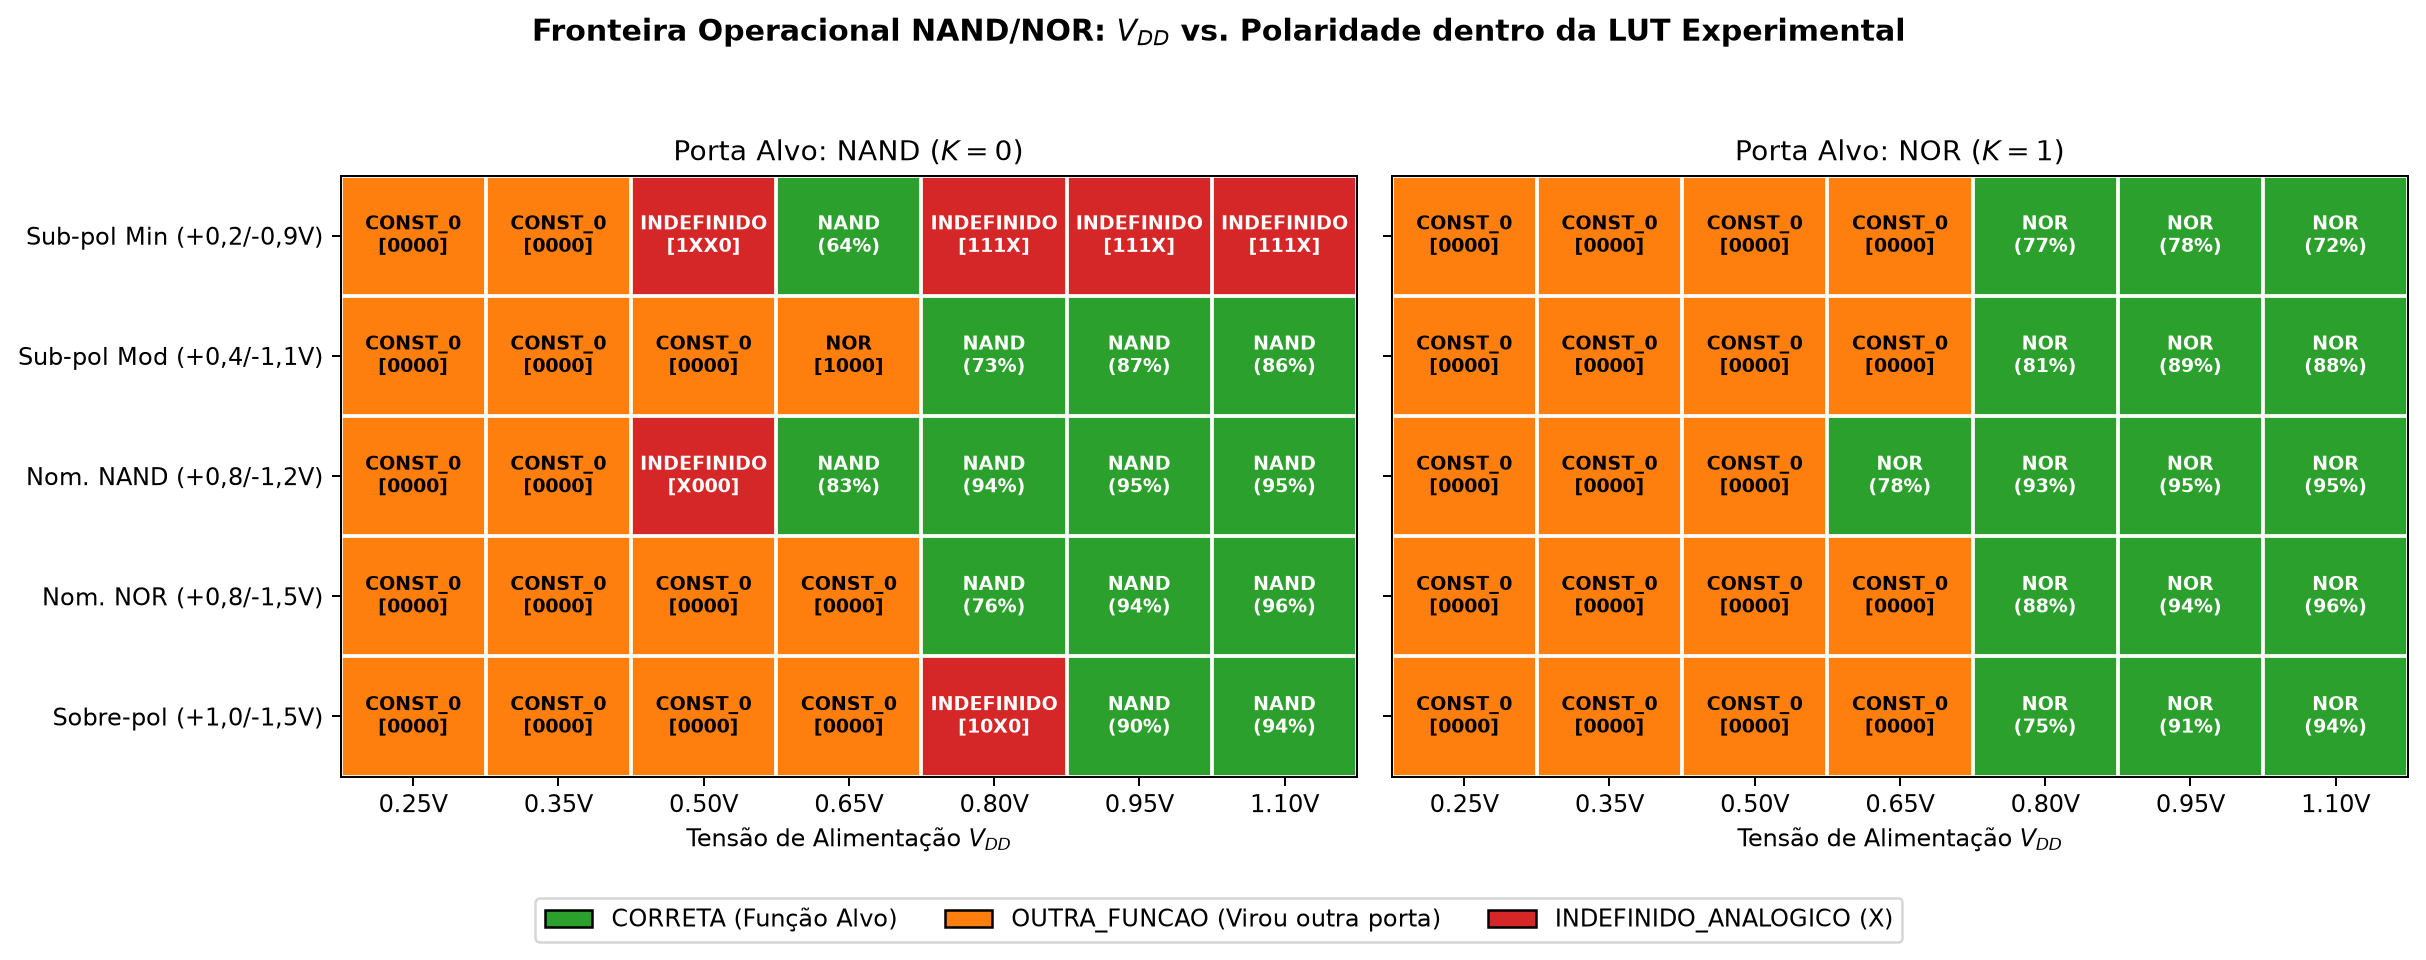
\includegraphics[width=0.92\textwidth]{m06_nand_nor_mapa_vdd_polaridade.png}
\caption{Operating phase map ($V_{DD} \times$ polarity) of the \texttt{NAND}/\texttt{NOR} gate, highlighting spontaneous \texttt{NAND} $\to$ \texttt{NOR} conversion at $V_{DD}=0.65\ \text{V}$ and \texttt{CONST\_0} collapse at under-voltage.}
\label{fig:m06_nn_vdd}
\end{figure}

\begin{figure}[htbp]
\centering
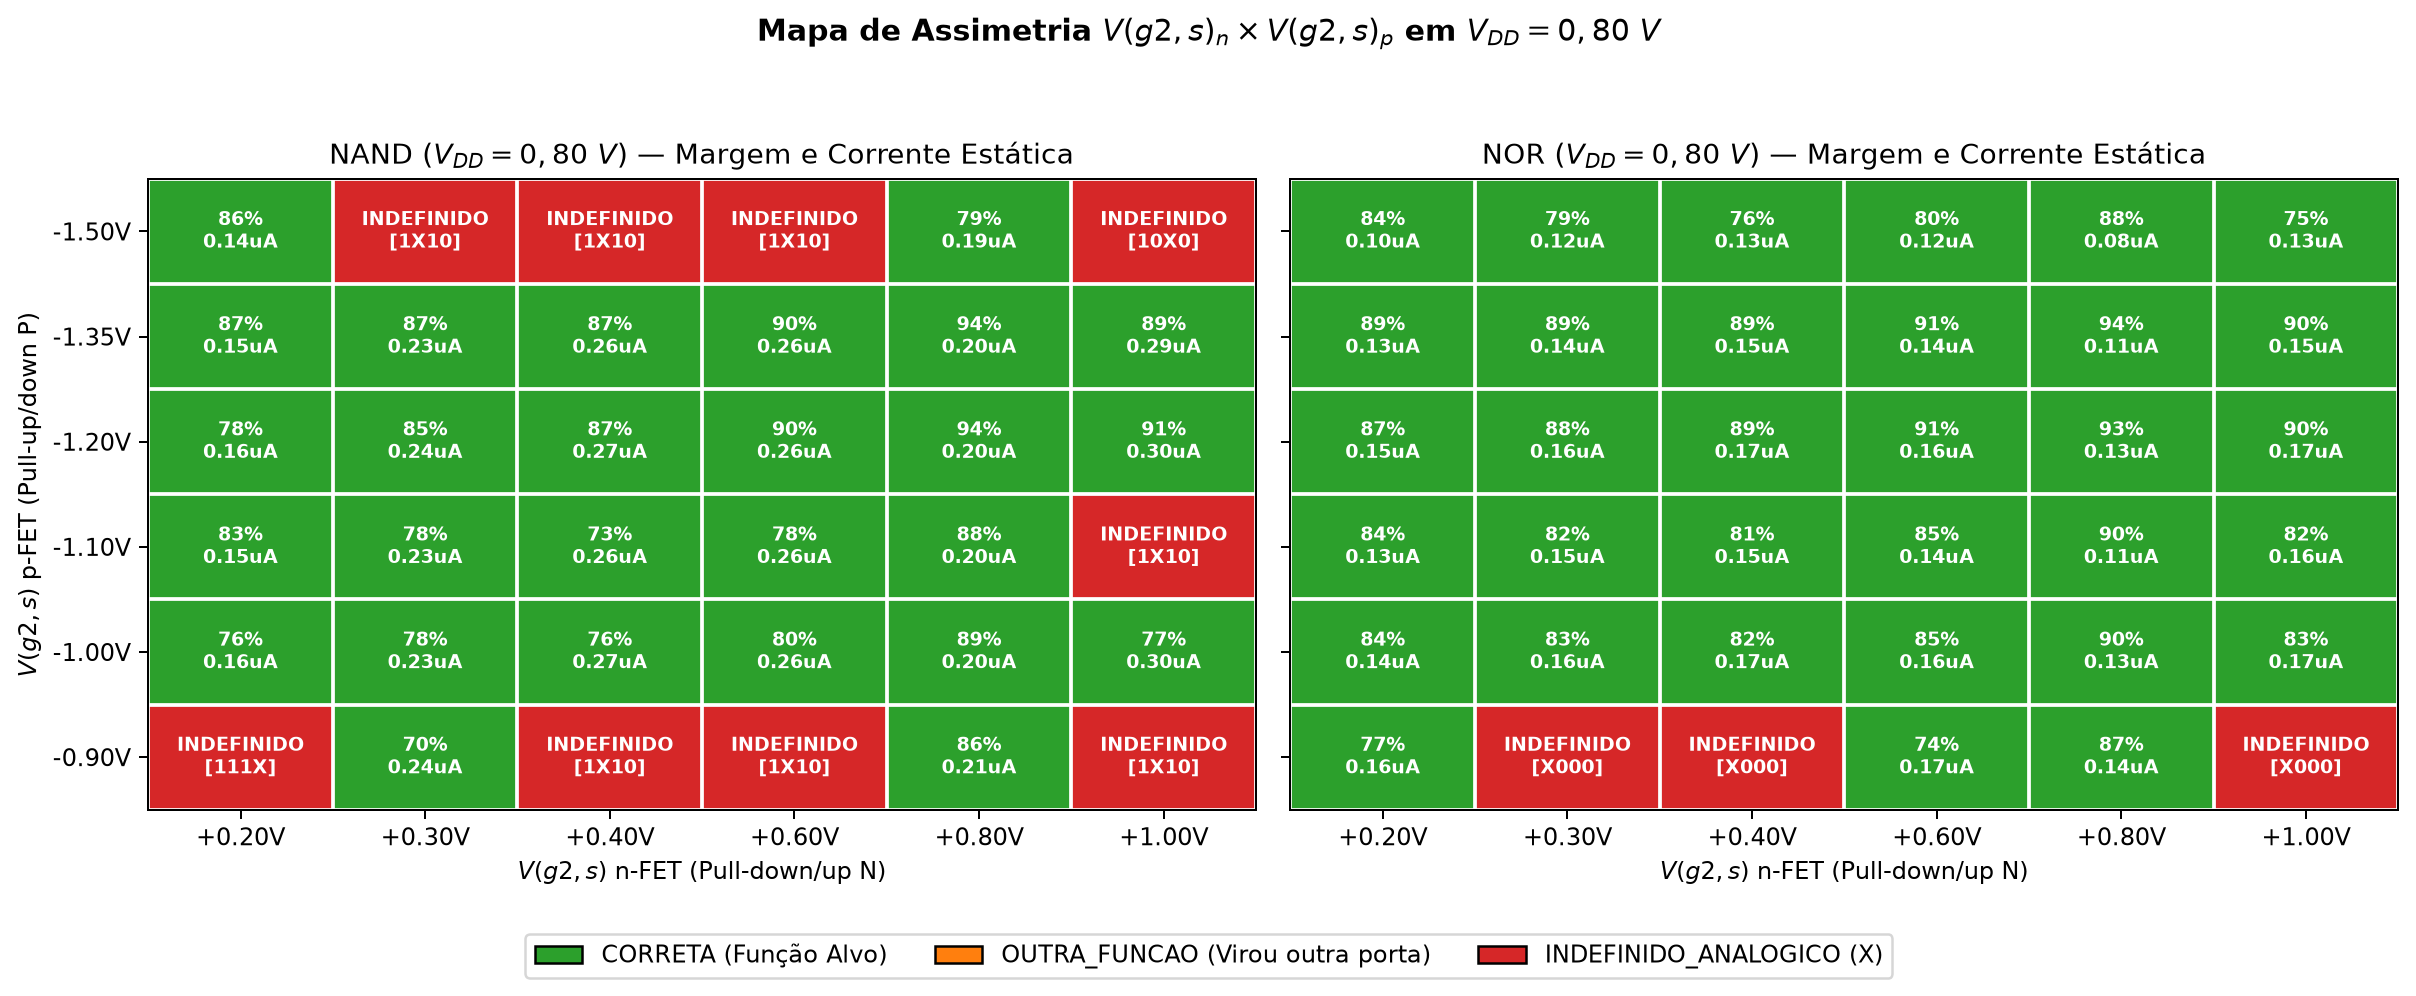
\includegraphics[width=0.92\textwidth]{m06_nand_nor_assimetria_vg2.png}
\caption{$V(g2,s)_n \times V(g2,s)_p$ asymmetry map at $V_{DD}=0.80\ \text{V}$ for \texttt{NAND} and \texttt{NOR}, exposing non-monotonic degradation at $V(g2,s)_p = -1.50\ \text{V}$.}
\label{fig:m06_nn_asym}
\end{figure}

\begin{figure}[htbp]
\centering
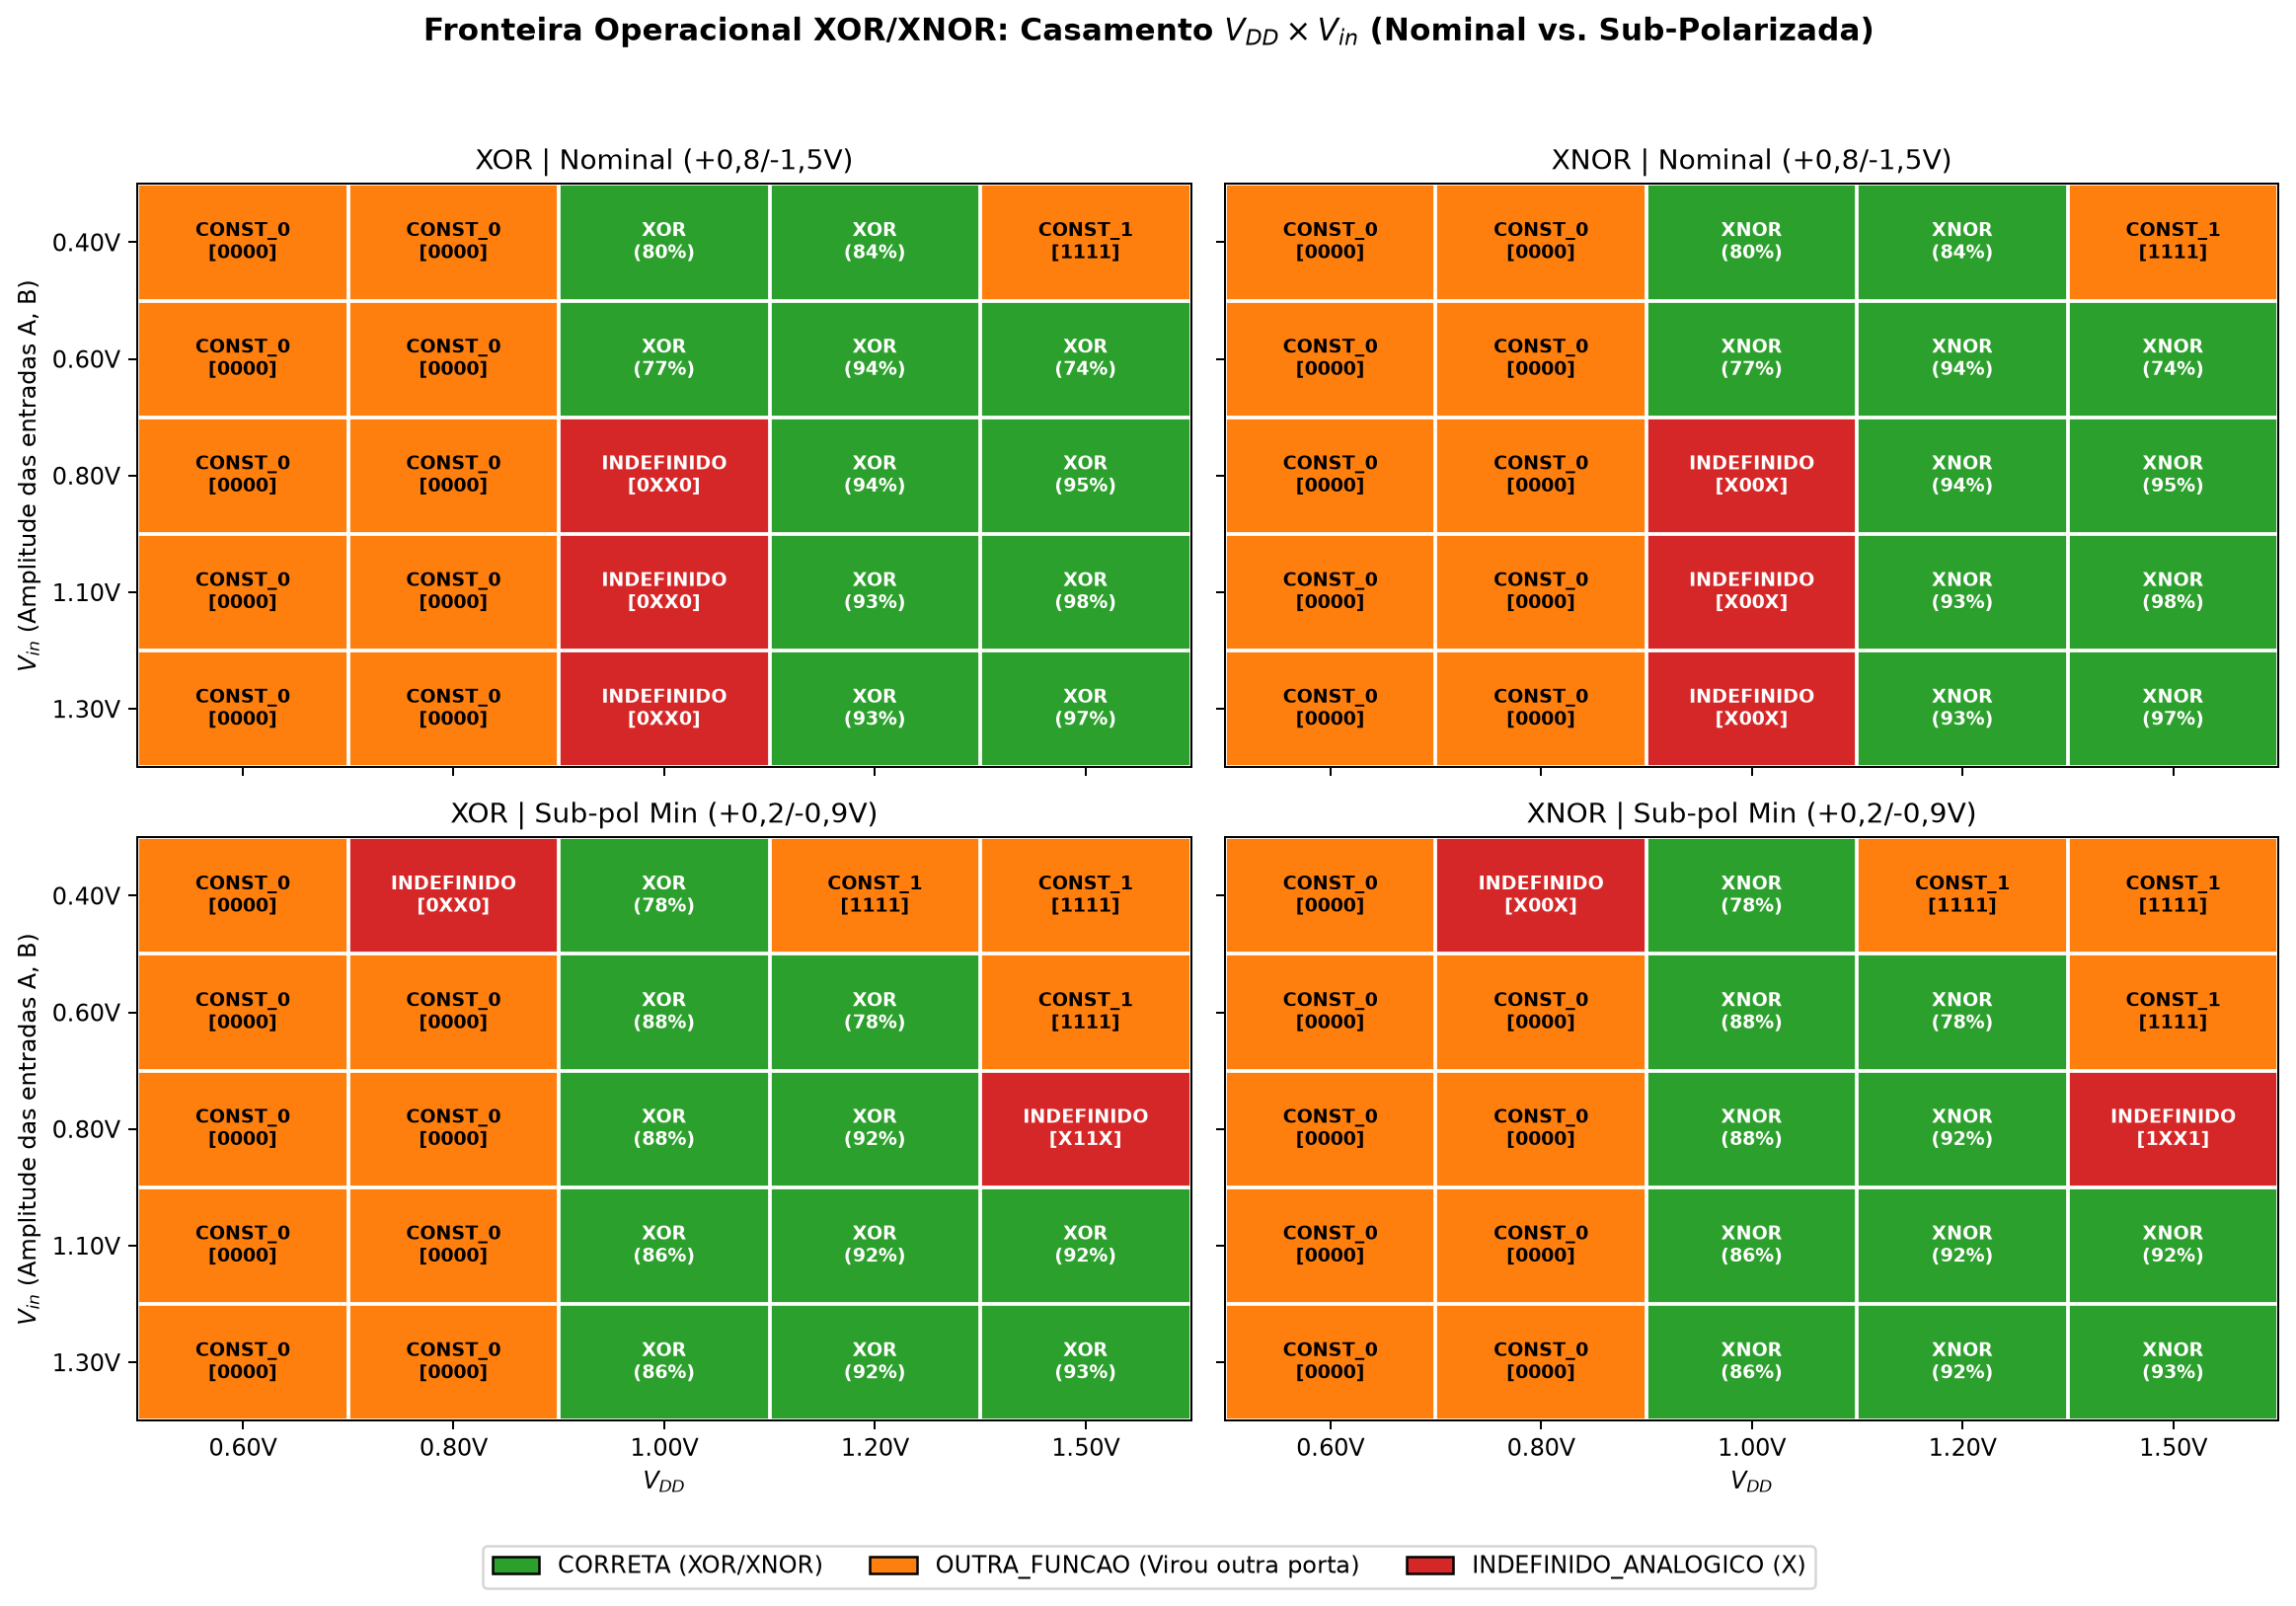
\includegraphics[width=0.92\textwidth]{m06_xor_xnor_mapa_vdd_vin.png}
\caption{$V_{DD} \times V_{\mathrm{in}}$ operating map of the \texttt{XOR}/\texttt{XNOR} gate under nominal bias, sub-polarization, and fixed gate voltage, illustrating \texttt{CONST\_0}, \texttt{CONST\_1}, and undefined regions.}
\label{fig:m06_xor_map}
\end{figure}

\subsection{DPA Asymmetry across Seven Polymorphic Tuples and Full Adder Benchmark}\label{sec:res_tuples}

In Module~\texttt{07}, all $72$ input-key combinations across the seven polymorphic tuples achieved $100.0\%$ functional correctness ($V_{1,\min} \ge 0.6792\ \text{V}$ at $0.8\ \text{V}$ and $\ge 1.3767\ \text{V}$ at $1.5\ \text{V}$; $V_{0,\max} \le 0.0128\ \text{V}$). Table~\ref{tab:tuples_dpa} compiles the hardware cost, DPA asymmetry, dynamic performance, and Monte Carlo robustness metrics.

\begin{table}[htbp]
\centering
\caption{Consolidated cost, DPA asymmetry, dynamic performance, and Monte Carlo robustness across seven polymorphic tuples ($C_{\mathrm{load}} = 0.3\ \text{fF}$).}
\label{tab:tuples_dpa}
\resizebox{\textwidth}{!}{%
\begin{tabular}{l c c c c c c c c c c c}
\toprule
\textbf{Tuple} & \textbf{Core/Tot.} & $\sum W$ ($\mu\text{m}$) & $V_{DD}$ (V) & $I_{\mathrm{peak}}$ M0/M1 ($\mu\text{A}$) & \textbf{Peak DPA} & \textbf{Avg.\ DPA} & $t_p$ (ps) & $P_{\mathrm{avg}}$ (nW) & $E_{\mathrm{sw}}$ (fJ) & \textbf{PDP} (aJ) & \textbf{MC} ($N=250$) \\
\midrule
\texttt{(NAND, NOR)}   & 4T / 4T   & $6.0$  & $0.8$ & $0.5643$ / $0.2138$ & $163.91\%$ & $44.62\%$ & $554.28$ & $40.17$  & $0.5022$ & $22.27$ & $100.00\%$ \\
\texttt{(XOR, XNOR)}   & 4T / 8T   & $4.0$  & $1.5$ & $1.6914$ / $1.6914$ & $0.00\%$   & $30.57\%$ & $151.84$ & $102.47$ & $1.2808$ & $15.56$ & $100.00\%$ \\
\texttt{(AND, OR)}     & 6T / 6T   & $9.0$  & $0.8$ & $1.7345$ / $1.8394$ & $6.05\%$   & $30.87\%$ & $454.27$ & $48.04$  & $0.6005$ & $21.82$ & $100.00\%$ \\
\texttt{(NAND, XNOR)}  & 6T / 10T  & $8.0$  & $1.5$ & $1.7050$ / $1.3387$ & $27.36\%$  & $73.87\%$ & $163.46$ & $94.14$  & $1.1768$ & $15.39$ & $100.00\%$ \\
\texttt{(NOR, XOR)}    & 6T / 10T  & $8.0$  & $1.5$ & $1.7129$ / $1.6932$ & $1.16\%$   & $29.60\%$ & $144.87$ & $121.49$ & $1.5186$ & $17.60$ & $100.00\%$ \\
\texttt{(AOI21, OAI21)}& 6T / 6T   & $12.0$ & $0.8$ & $0.6810$ / $0.4299$ & $58.44\%$  & $19.22\%$ & $555.72$ & $59.97$  & $0.4498$ & $33.33$ & $99.55\%$  \\
\texttt{(MAJ3, XOR3)}  & 10T / 18T & $18.0$ & $1.5$ & $1.4360$ / $1.4355$ & $0.04\%$   & $47.08\%$ & $180.71$ & $212.44$ & $1.9119$ & $38.39$ & $100.00\%$ \\
\bottomrule
\end{tabular}}
\end{table}

Under the standardized \texttt{ngspice-47} testbench, the current traces (Figure~\ref{fig:m07_signatures}) and Pareto frontier (Figure~\ref{fig:m07_pareto}) reveal distinct design trade-offs:
\begin{itemize}
    \item \texttt{(NAND, NOR)} achieves minimal physical cost ($4\text{T}$, $40.17\ \text{nW}$) at the expense of severe peak DPA exposure ($163.91\%$) and high delay ($554.28\ \text{ps}$) caused by asymmetry between parallel ($W=1.0$) and series ($W=2.0$) stacks.
    \item \texttt{(XOR, XNOR)} completely eliminates peak asymmetry ($0.00\%$, $1.6914\ \mu\text{A}$ in both modes) with a low PDP of $15.56\ \text{aJ}$.
    \item In \texttt{(AND, OR)}, appending the \texttt{BP\_INV08} output inverter ($+2\text{T}$) isolates the load from the polymorphic core and reduces overall supply peak asymmetry to $6.05\%$, although asymmetry across $1 \to 0$ falling edges remains substantial ($116.90\%$).
    \item Among mixed-locking cells, \texttt{(NOR, XOR)} offers an outstanding trade-off ($1.16\%$ peak DPA asymmetry and the lowest delay in the suite at $144.87\ \text{ps}$), whereas \texttt{(NAND, XNOR)} exhibits high average asymmetry ($73.87\%$) due to the \texttt{'1'}-probability imbalance between \texttt{NAND} ($75\%$) and \texttt{XNOR} ($50\%$).
    \item For 3-input cells, \texttt{(AOI21, OAI21)} delivers the lowest time-averaged asymmetry ($19.22\%$) and lowest switching energy ($0.4498\ \text{fJ}$) in $6\text{T}$, with a slight Monte Carlo drop ($99.55\%$, Figure~\ref{fig:m07_mc}) under stacked \texttt{OAI21} conduction; conversely, \texttt{(MAJ3, XOR3)} extends quad-symmetric balance to three inputs with $0.04\%$ peak DPA asymmetry and $100.0\%$ Monte Carlo yield.
\end{itemize}

\begin{figure}[htbp]
\centering
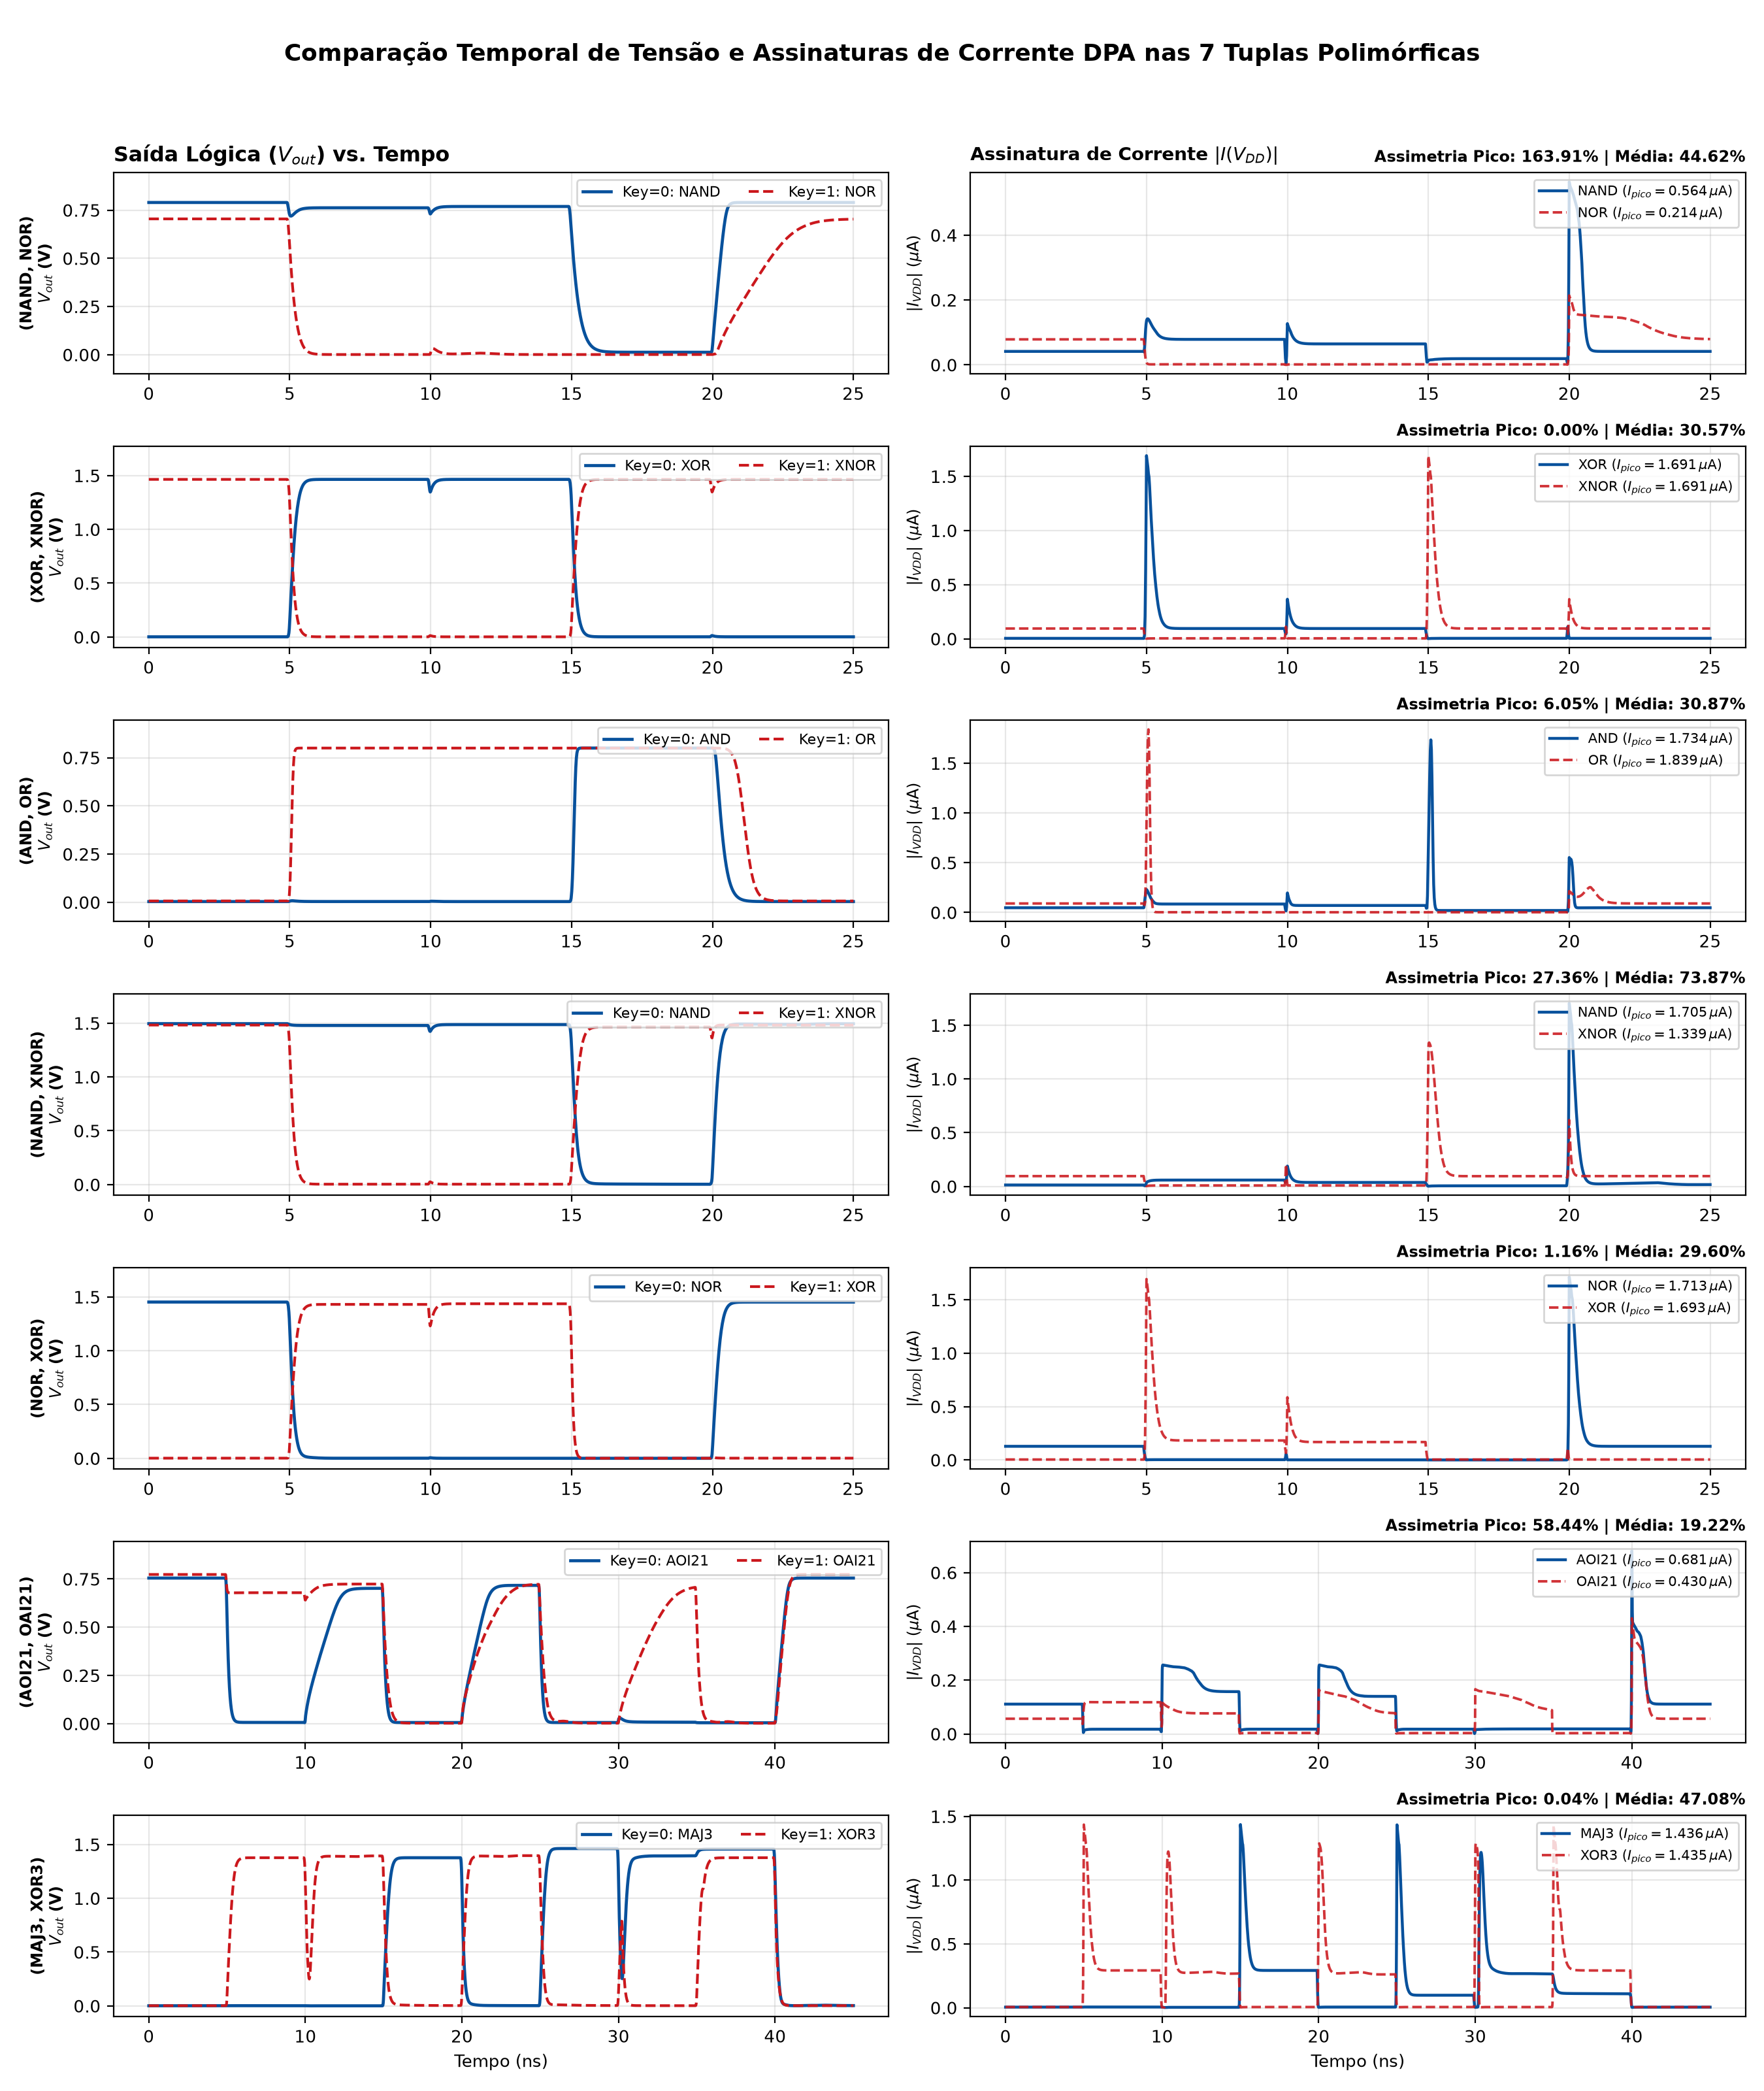
\includegraphics[width=0.90\textwidth,height=0.76\textheight,keepaspectratio]{m07_assinaturas_corrente_tuplas.png}
\caption{Supply current signatures $|I(V_{DD})|$ comparing $\text{Key}=0$ and $\text{Key}=1$ across the seven polymorphic tuples under standardized capacitive load ($C_{\mathrm{load}} = 0.3\ \text{fF}$).}
\label{fig:m07_signatures}
\end{figure}

\begin{figure}[htbp]
\centering
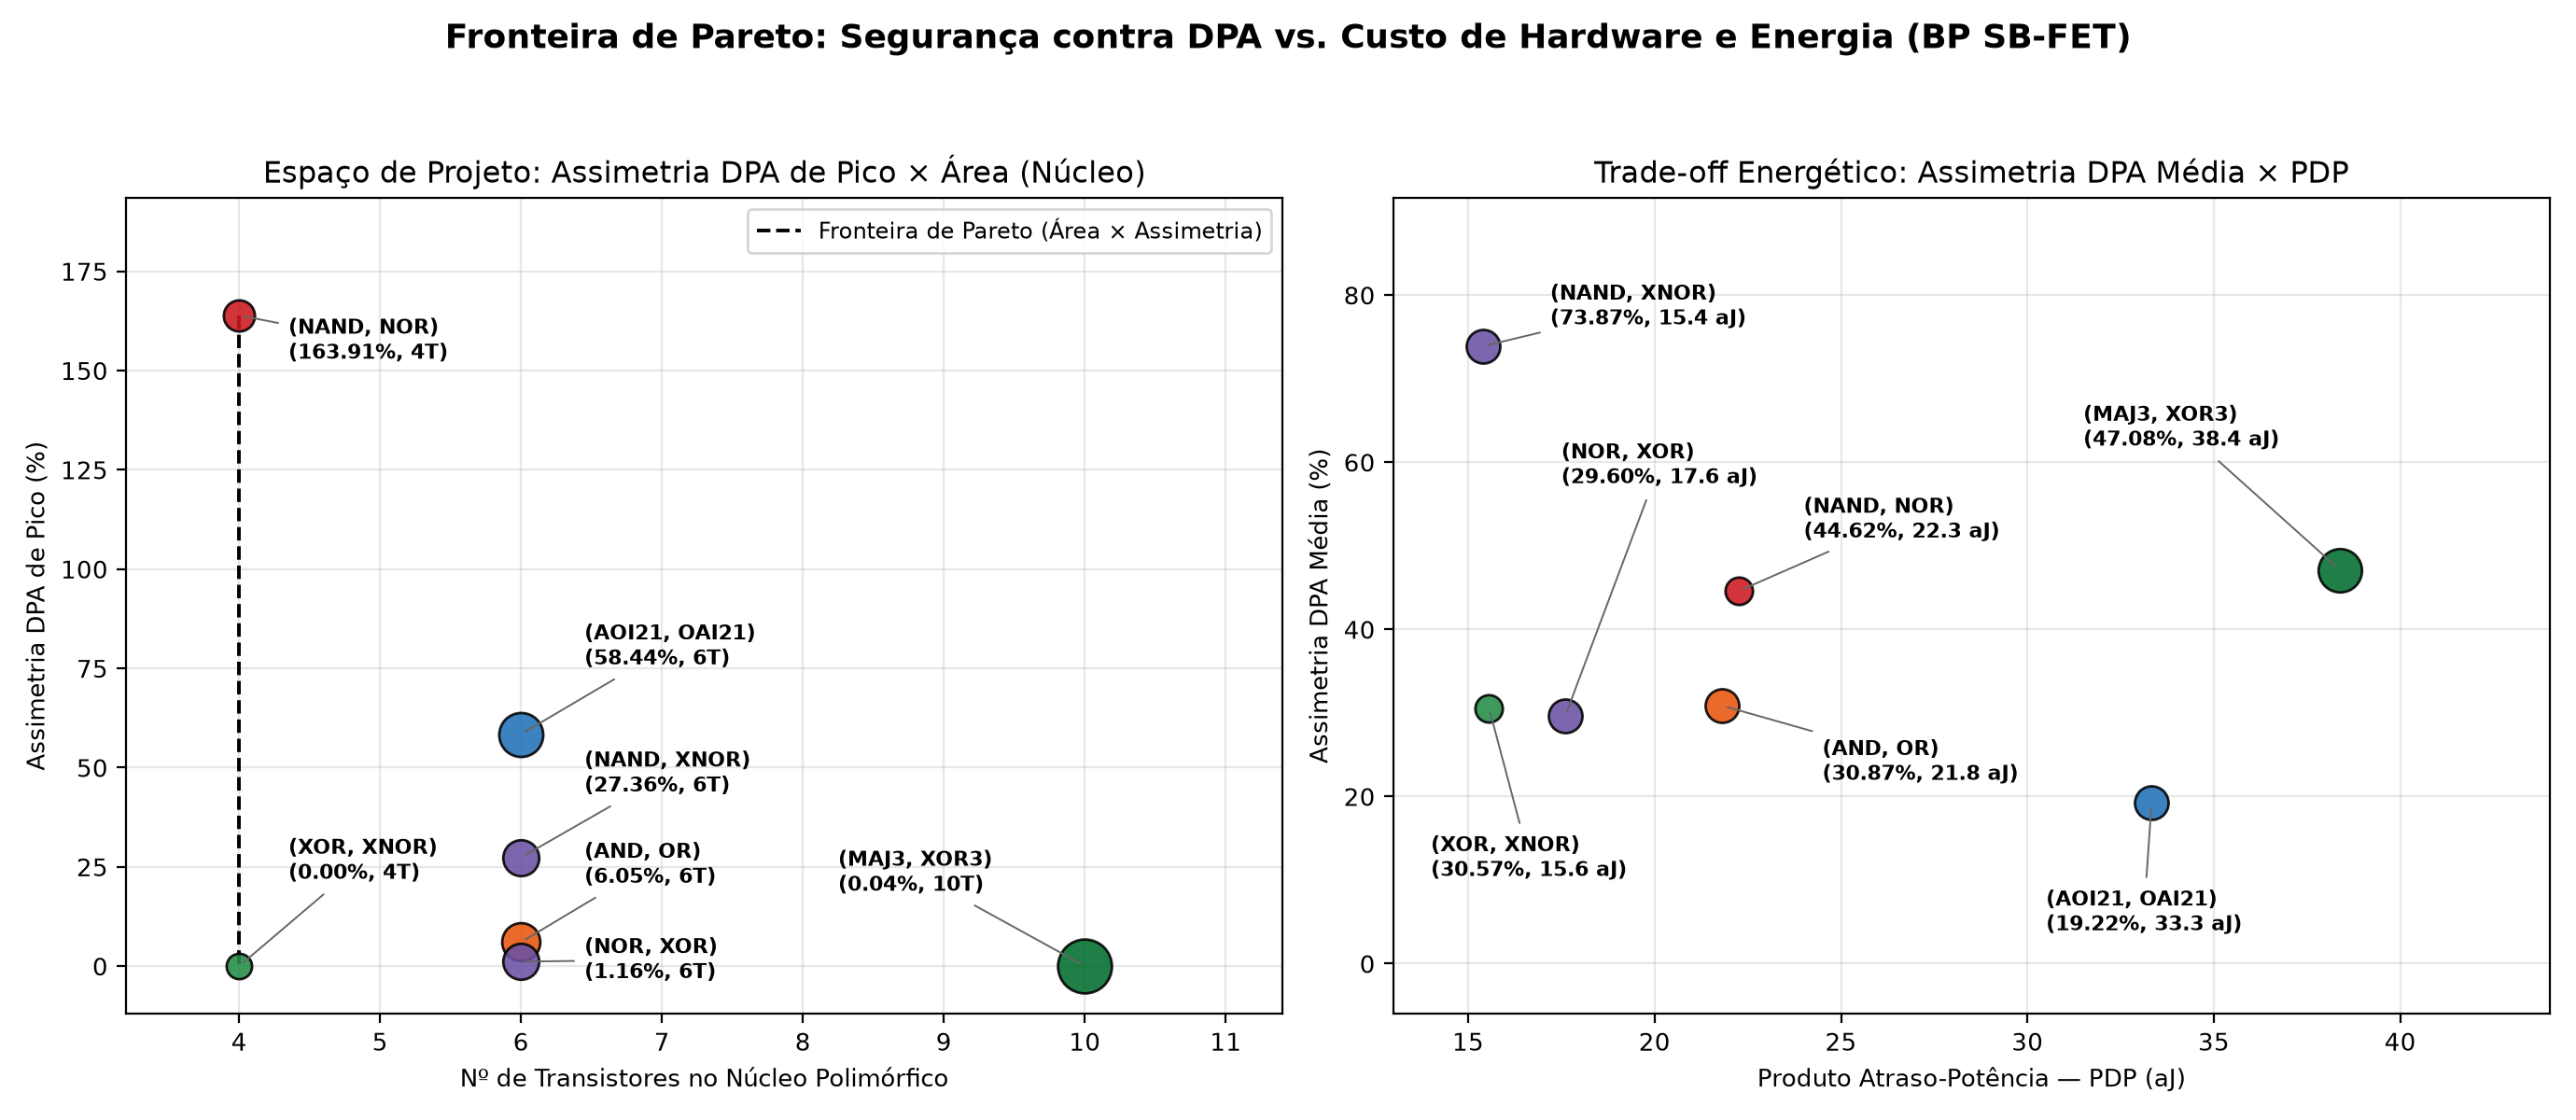
\includegraphics[width=0.92\textwidth]{m07_pareto_assimetria_vs_custo.png}
\caption{Pareto frontier relating peak DPA asymmetry, transistor count, and power-delay product ($\mathrm{PDP}$) across the seven evaluated tuples.}
\label{fig:m07_pareto}
\end{figure}

\begin{figure}[htbp]
\centering
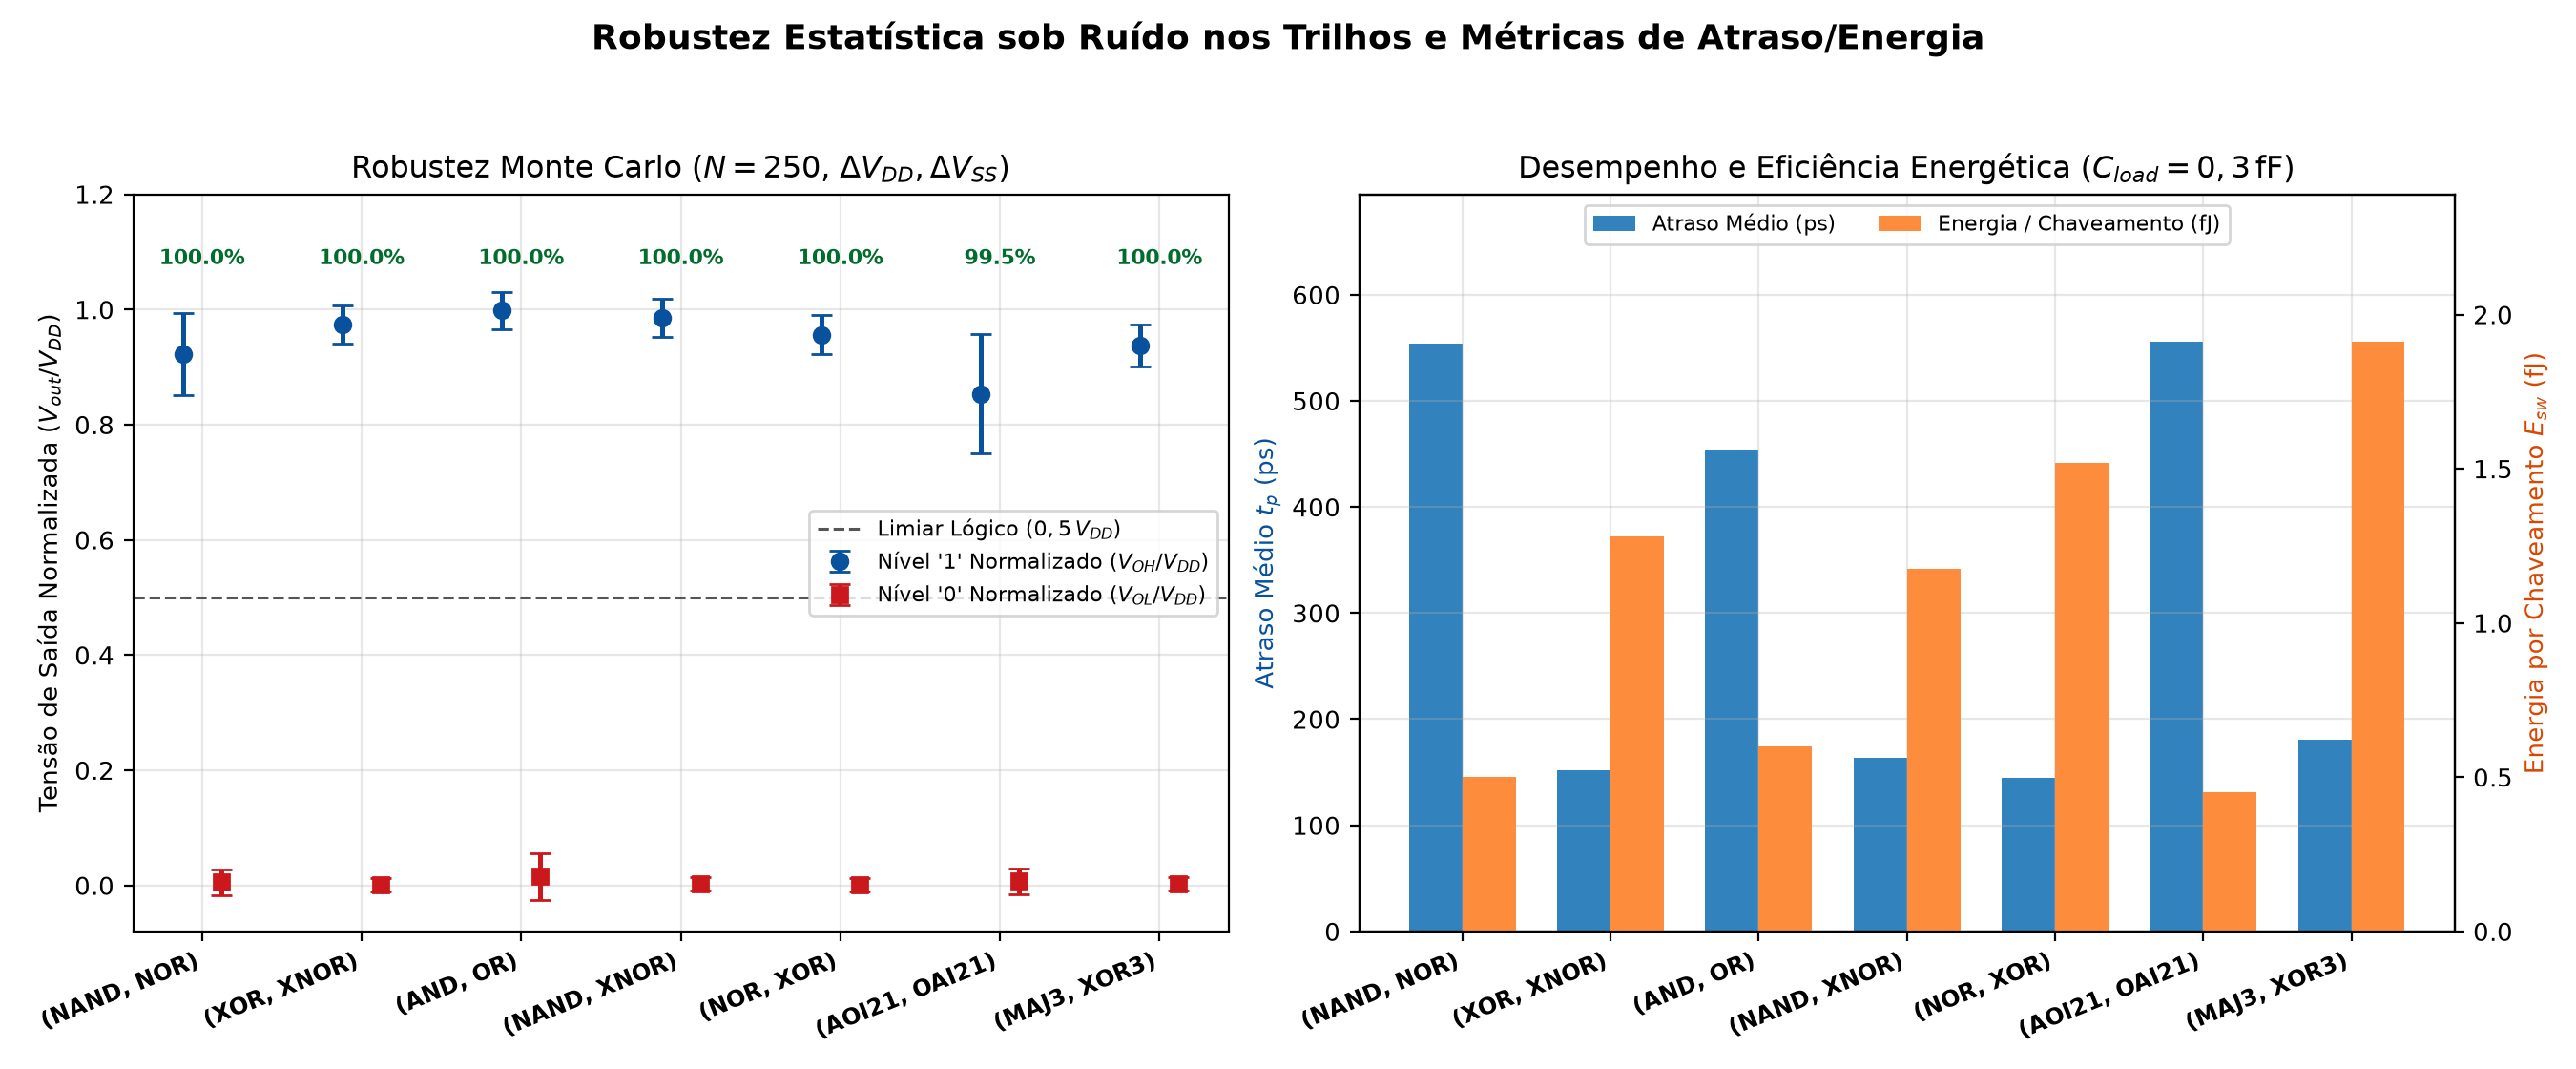
\includegraphics[width=0.92\textwidth]{m07_robustez_montecarlo_tuplas.png}
\caption{Monte Carlo yield ($N=250$) under realistic supply-rail noise and delay/energy distributions across the seven tuples.}
\label{fig:m07_mc}
\end{figure}

In the system-level 1-bit Full Adder benchmark (Table~\ref{tab:fa_profiles} and Figure~\ref{fig:m07_fa}), all three architectures achieved $100.0\%$ accuracy under $K=00$. \textbf{Profile 2} (using three \texttt{NAND}/\texttt{NOR} gates for carry) increases core count to 28T, multiplies critical delay by $3.58\times$ over the Baseline ($177.72 \to 636.68\ \text{ps}$), raises critical PDP by $3.54\times$ ($131.86 \to 466.44\ \text{aJ}$), and leaks a $113.83\%$ peak DPA signature on the carry stage. By contrast, \textbf{Profile 3} replaces the \texttt{NAND}/\texttt{NOR} tree with a single 10T \texttt{(MAJ3, XOR3)} gate, cutting core count to 26T, raising wrong-key ($K=11$) Hamming Distance from $68.75\%$ to $87.50\%$, and slashing peak DPA asymmetry in the polymorphic carry stage from $113.83\%$ down to just \textbf{$0.04\%$}. With a critical delay of $196.98\ \text{ps}$ ($+10.8\%$ over Baseline) and PDP of $155.19\ \text{aJ}$ ($+17.7\%$ over Baseline and \textbf{$3.01\times$ lower than Profile 2}), Profile 3 simultaneously excels in security, area, and energy efficiency.

\begin{table}[htbp]
\centering
\caption{System-level 1-bit Full Adder benchmark across three architectural profiles in \texttt{ngspice-47} ($C_{\mathrm{load}} = 0.3\ \text{fF}$).}
\label{tab:fa_profiles}
\resizebox{\textwidth}{!}{%
\begin{tabular}{l c c c c c c c c c}
\toprule
\textbf{Architectural Profile} & \textbf{Core} & $\sum W$ & \textbf{K00 Acc.} & \textbf{HD (K11)} & $t_{\mathrm{crit}}$ (ps) & $P_{\mathrm{avg}}$ (nW) & \textbf{PDP} (aJ) & \textbf{Carry Peak DPA} & \textbf{Carry Avg.\ DPA} \\
\midrule
1. Baseline (Common, unlocked) & 20T & $24.0$ & $100.0\%$ & $0.0\%$   & $177.72$ & $741.97$ & $131.86$ & N/A & N/A \\
2. Cost/Perf.\ (\texttt{NAND}/\texttt{NOR}) & 28T & $38.0$ & $100.0\%$ & $68.75\%$ & $636.68$ & $732.60$ & $466.44$ & $113.83\%$ & $62.44\%$ \\
3. Low Asymmetry (\texttt{MAJ3}/\texttt{XOR3}) & 26T & $38.0$ & $100.0\%$ & $87.50\%$ & $196.98$ & $787.87$ & $155.19$ & $0.04\%$   & $47.47\%$ \\
\bottomrule
\end{tabular}}
\end{table}

\begin{figure}[htbp]
\centering
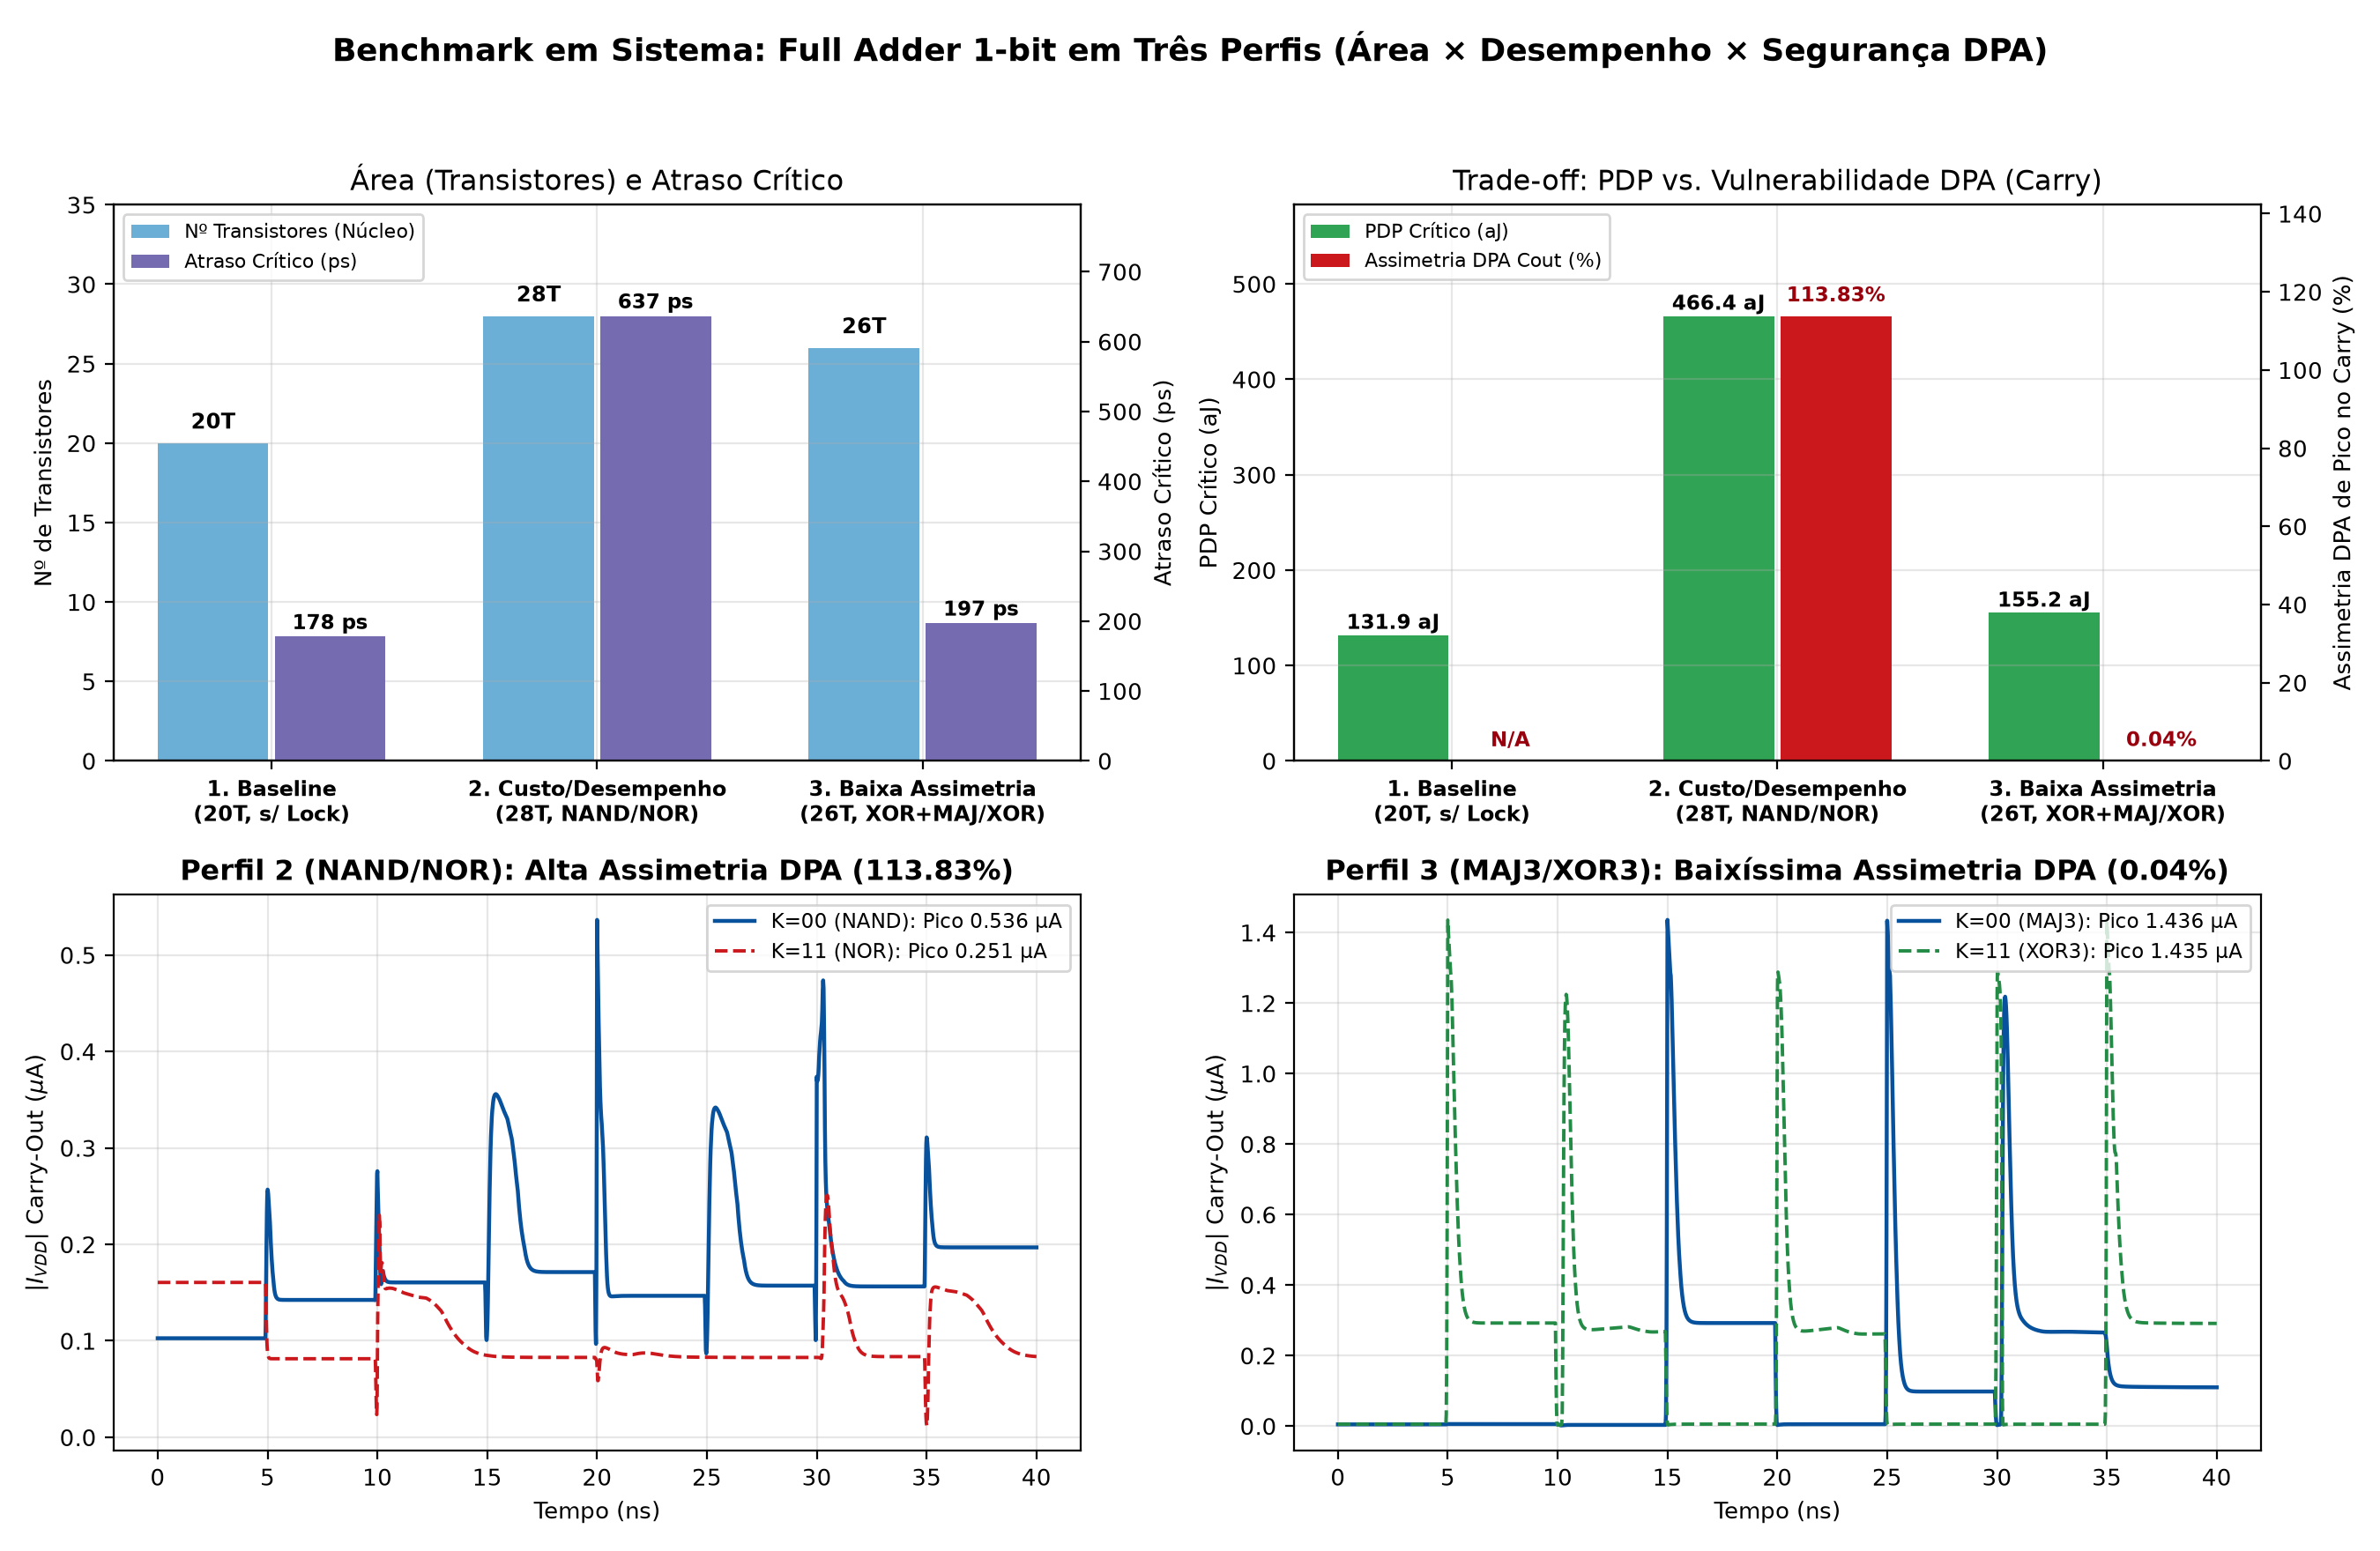
\includegraphics[width=0.92\textwidth]{m07_benchmark_full_adder_perfis.png}
\caption{Comparison of the three 1-bit Full Adder architectural profiles across transistor count, critical delay, PDP, wrong-key obfuscation (HD), and carry DPA asymmetry.}
\label{fig:m07_fa}
\end{figure}

\subsection{End-to-End Validation of the Interactive Visual Simulator (\textit{BP-FET Studio})}\label{sec:res_web}

The automated test suite \texttt{simulador\_web/test\_simulator.py} fully validated graph compilation, batch \texttt{ngspice-47} execution, and the REST backend of \textit{BP-FET Studio}:
\begin{enumerate}
    \item \textbf{Seven polymorphic tuples and \texttt{INV} at high level:} every truth-table row and \textit{X-Ray} transistor mapping passed with $100\%$ accuracy, reproducing the Module~\texttt{07} peak DPA asymmetry metrics (\texttt{NAND\_NOR}: $163.91\%$; \texttt{XOR\_XNOR}: $0.00\%$; \texttt{AND\_OR}: $6.05\%$; \texttt{NAND\_XNOR}: $27.36\%$; \texttt{NOR\_XOR}: $1.16\%$; \texttt{AOI21\_OAI21}: $58.44\%$; \texttt{MAJ3\_XOR3}: $0.04\%$; \texttt{INV}: $0.00\%$) in execution times from $234\ \text{ms}$ (\texttt{INV}) to $7.04\ \text{s}$ (\texttt{MAJ3\_XOR3}).
    \item \textbf{Eight catalog templates:} all high- and low-level circuits passed ($0.65\ \text{s}$ to $14.31\ \text{s}$), verifying both Full Adder Profiles 2 and 3 at $K=0$, physical polarity flipping (\textit{p-FET} $\leftrightarrow$ \textit{n-FET}) in the 4T \texttt{NAND}/\texttt{NOR} cell, and retention ($\Delta V > 0.7\ \text{V}$ at $12\ \text{ns}$, \texttt{XPU1} as \textit{p-FET}) followed by collapse ($\Delta V < 0.25\ \text{V}$ at $28\ \text{ns}$, \texttt{XPU1} as \textit{n-FET}) in the 6T SRAM.
    \item \textbf{Mixed multi-domain cascade and HTTP API:} an arbitrary mixed-voltage chain $0.8\ \text{V} \to 1.5\ \text{V} \to 0.8\ \text{V}$ (\texttt{NAND\_\allowbreak NOR} $\to$ \texttt{XOR\_\allowbreak XNOR} $\to$ \texttt{AND\_\allowbreak OR}) with automatic level conditioning compiled and passed in $5.87\ \text{s}$ ($100\%$ exact for $\text{Key}=0$ and $\text{Key}=1$), and all HTTP/JSON endpoints (\texttt{/}, \texttt{/api/\allowbreak tuples}, \texttt{/api/\allowbreak templates}, \texttt{/api/\allowbreak simulate}) returned HTTP $200$.
\end{enumerate}
